\documentclass[twoside,a4paper,12pt]{book}%,AutoFakeBold,twoside,openright,
% 可用选项有 debug|ebook|hardcopy, amd|pmd|phdplain|phdfancy, nobox, manualSpine, onlyCover, twoSideCover, noBlankPages.
% debug 生成的PDF带框线,方便调试
% ebook 带彩色文字的PDF
% hardcopy 无彩色文字的PDF
% amd 学硕使用
% pmd 专硕使用
% phdplain 博士论文简装
% phdfancy 博士论文精装
% nobox 输出的封面无框线和书脊
% manualSpine 手动输出书脊,需配合\jluManualSpine命令
% onlyCover 仅输出封面页
% twoSideCover 输出双页封面
% noBlankPages 去掉空白页,主要用于上传到图书馆学位论文系统
% 默认为 hardcopy,amd,且nobox=false,manualSpine=false,onlyCover=false,twoSideCover=false, noBlankPages=false
% 双面印刷需在documentclass选项中声明twoside
% 单面印刷需在documentclass选项中声明oneside
% 选项使用举例如下\usepackage{xeCJK}
%\usepackage[phdplain,ebook,twoSideCover,onlyCover]{jluthesis2020}%
%\usepackage[amd,hardcopy,twoSideCover]{jluthesis2020}%
\usepackage[phdfancy,hardcopy,noBlankPages]{jluthesis2020}%
%\usepackage[phdplain,hardcopy,noBlankPages]%
\usepackage{xeCJK}
\usepackage{amsmath}
\usepackage{xcolor}
% 用于算法注释
\usepackage{algcompatible}
\renewcommand{\COMMENT}[2][.5\linewidth]{%
  \leavevmode\hfill\makebox[#1][l]{//~#2}}
\algnewcommand\algorithmicto{\textbf{to}}
\algnewcommand\RETURN{\State \textbf{return} }
\usepackage{fancyhdr}
%\fancyhead[L,R]{~\thepage~} % 在偶数页的左侧,奇数页的右侧显示页码
% 用于排版代码
\usepackage{hyperxmp}
\usepackage{listings}
\usepackage{amsmath}

\usepackage{glossaries}
\usepackage{glossaries-extra}
\makeglossaries


\newtheorem{example}{例}
\newtheorem{definition}{定义}
\newtheorem{axiom}{公理}
\newtheorem{property}{性质}
\newtheorem{proposition}{命题}
\newtheorem{lemma}{引理}
\newtheorem{corollary}{推论}
\newtheorem{remark}{注解}
\newtheorem{condition}{条件}
\newtheorem{conclusion}{结论}
\newtheorem{assumption}{假设}

\lstset{
    basicstyle          =   \sffamily,          % 基本代码风格
    keywordstyle        =   \bfseries,          % 关键字风格
    commentstyle        =   \rmfamily\itshape,  % 注释的风格,斜体
    stringstyle         =   \ttfamily,  % 字符串风格
    flexiblecolumns,                % 别问为什么,加上这个
    numbers             =   left,   % 行号的位置在左边
    showspaces          =   false,  % 是否显示空格,显示了有点乱,所以不现实了
    numberstyle         =   \zihao{-5}\ttfamily,    % 行号的样式,小五号,tt等宽字体
    showstringspaces    =   false,
    captionpos          =   t,      % 这段代码的名字所呈现的位置,t指的是top上面
    frame               =   lrtb,   % 显示边框
}

\lstdefinestyle{Python}{
    language        =   Python, % 语言选Python
    basicstyle      =   \zihao{-5}\ttfamily,
    numberstyle     =   \zihao{-5}\ttfamily,
    keywordstyle    =   \color{blue},
    keywordstyle    =   [2] \color{teal},
    stringstyle     =   \color{magenta},
    commentstyle    =   \color{red}\ttfamily,
    breaklines      =   true,   % 自动换行,建议不要写太长的行
    columns         =   fixed,  % 如果不加这一句,字间距就不固定,很丑,必须加
    basewidth       =   0.5em,
}
\definecolor{commentColor}{rgb}{0.0, 0.5, 0.0}
\lstset{ %
    language=Python,                % the language of the code
    basicstyle=\scriptsize\ttfamily,           % the size of the fonts that are used for the code
    numbers=left,                   % where to put the line-numbers
    numberstyle=\tiny\color{gray},  % the style that is used for the line-numbers
    stepnumber=2,                   % the step between two line-numbers. If it's 1, each line 
    % will be numbered
    numbersep=5pt,                  % how far the line-numbers are from the code
    backgroundcolor=\color{white},      % choose the background color. You must add \usepackage{color}
    showspaces=false,               % show spaces adding particular underscores
    showstringspaces=false,         % underline spaces within strings
    showtabs=false,                 % show tabs within strings adding particular underscores
    rulecolor=\color{black},        % if not set, the frame-color may be changed on line-breaks within not-black text (e.g. commens (green here))
    tabsize=2,                      % sets default tabsize to 2 spaces
    captionpos=b,                   % sets the caption-position to bottom
    breaklines=true,                % sets automatic line breaking
    breakatwhitespace=false,        % sets if automatic breaks should only happen at whitespace
                 % show the filename of files included with \lstinputlisting;
    % also try caption instead of title
    keywordstyle=\color{blue},          % keyword style
    commentstyle=\color{commentColor},       % comment style
    stringstyle=\color{black},         % string literal style
    escapeinside={(*}{*)},            % if you want to add LaTeX within your code
    morekeywords={*,...}               % if you want to add more keywords to the set
}
\newcommand{\commentMath}[1]{$\color{commentColor}#1$}

\graphicspath{{figures/}}


\begin{document}
\frontmatter
\sloppy % 解决中英文混排的断行问题,会加入间距,但不会影响断行 ????


% 手动在长标题中利用 \par 输入断行,
\jluCTitle{\Title}

% 竖排的书脊输出时,如果遇到中英混杂的标题会比较麻烦,需要中英分开控制输出
% 但如果仅有中文或英文都比较简单,如
% \jluCSpineTitle{吉林大学学位论文模版示例} % 仅中文的书脊标题
% \jluCSpineTitle{\jluPrintSpine{Sample Typesetting for {\jluthesisVersion}}} % 仅英文的书脊标题
\jluCSpineTitle{\jluPrintSpine{\jluPrintSpineChinese{自然语言处理综述}{\jluthesisVersion}\jluPrintSpineChinese{示例}}} % 中英混杂的书脊标题
\author{曹玉吉}
\jluSpineHorizontalPosition{1.65} % 书脊的水平位置,修改可使书脊水平平移




\hypersetup{
	pdfcreator={XeLaTeX \& \jluthesisVersion},   % creator of the document
	pdfproducer={XeLaTeX \& \jluthesisVersion},  % producer of the document
	pdfinfo={
          CreationDate={2020 0401 120000},
          ModDate={2020 0401 120000},
    },
}
%\jluMakeCover


%\titleformat{\chapter}{\centering\sffamily\mdseries\sanhao}{\CJKchaptername}{1em}{}
%\titlespacing{\chapter}{0pt}{8pt}{16pt}
\pagenumbering{Roman} 
\begin{titlepage}
	\begin{center}
		\hfill\\
		\vspace{1cm}
		% title of this document
		{\fontsize{36pt}{44pt}\bfseries 神经网络自然语言处理}\\
		\vspace{1em}
		{\LARGE\href{http://neuralnetworksanddeeplearning.com/index.html}{Natural Language Processing with Neural Networks}}\\
		\vspace{1cm}
		
\includegraphics{cayley}\\
		\vspace{1cm}
		{\LARGE \href{http://michaelnielsen.org/}{曹玉吉} 著}\\
		\vspace{1cm}
		%{\Large
		%	\begin{tabular}{rl}
		%		\href{mailto:xhzhu.nju@gmail}{Xiaohu Zhu} & \multirow{2}{*}{译} \\
		%		\href{mailto:zhanggyb@gmail.com}{Freeman Zhang} & \\
		%	\end{tabular}
		%}\\
		\vfill
		\vfill
		\vfill
		%{\large \today}\\
		\vspace{1em}
		{\large 版本: \href{https://github.com/zhanggyb/nndl/releases/tag/0.5}{1.0}}
	\end{center}
\end{titlepage}

\chapter{关于作者}
\label{ch:Author}

\begin{minipage}{0.7\linewidth}
	\textbf{曹玉吉 Gavin CAO} 是一位长期从事计算机编程、算法优化和自然语言处理技术工程师。目前就职于北京嘀嘀无限科技发展有限公司,目前负责顺风车事业部的服务管控算法方向的算法研发工作。
\end{minipage}
\hfill
\begin{minipage}{0.25\linewidth}
	
\includegraphics[width=0.99\linewidth]{author}  
\end{minipage}



\tableofcontents

\newglossaryentry{RNN}{name={RNN},description={Recurrent neural networks}}
\newglossaryentry{CNN}{name={CNN},description={Convolutional neural networks}}
\newglossaryentry{BERT}{name={BERT},description={Bidirectional encoder representation from transformer}}
\newglossaryentry{GPT}{name={GPT},description={Generative pre-training}}
\newglossaryentry{CBOW}{name={CBOW},description={Continuous bag of words}}
\newglossaryentry{BPE}{name={BPE},description={Bytes pair encoding}}
\newglossaryentry{Glove}{name={Glove},description={Global vectors for word representation}}
\newglossaryentry{SAN}{name={SAN},description={Self attention networks}}
\newglossaryentry{NMT}{name={NMT},description={Neural machine translation}}
\newglossaryentry{MRC}{name={MRC},description={Machine reading comprehension}}
\newglossaryentry{ASR}{name={ASR},description={Automatic speech recognition}}
\newglossaryentry{HMM}{name={HMM},description={Hidden markov model}}
\newglossaryentry{CRF}{name={CRF},description={Conditional random field}}
\newglossaryentry{LAN}{name={LAN},description={Label attention network}}
\newglossaryentry{OOV}{name={OOV},description={Out of Vocabulary}}
\newglossaryentry{LSTM}{name={LSTM},description={Long short term memory network}}
\newglossaryentry{GRU}{name={GRU},description={Gated recurrent unit}}
\newglossaryentry{IDCNN}{name={IDCNN},description={Iterated Dilated CNN}}
\newglossaryentry{NLU}{name={NLU},description={Natural language understanding}}
\newglossaryentry{NLP}{name={NLP},description={Natural language processing}}
\newglossaryentry{NER}{name={NER},description={Named entity recognition}}
\newglossaryentry{RNNLM}{name={RNNLM},description={Recurrent neural networks language model}}
\newglossaryentry{CNNLM}{name={CNNLM},description={Convolutional neural networks language model}}
\newglossaryentry{NNLM}{name={NNLM},description={Neural networks language model}}
\newglossaryentry{VDCNN}{name={VDCNN},description={Very deep convolutional neural networks}}
\newglossaryentry{LDA}{name={LDA},description={Latent dirichlet allocation}}
\newglossaryentry{LSA}{name={LSA},description={Latent semantic analysis}}
\newglossaryentry{SVM}{name={SVM},description={Support vector machine}}
\newglossaryentry{HAN}{name={HAN},description={Hierarchical attention networks}}
\newglossaryentry{MLM}{name={MLM},description={Masked language mode}}
\newglossaryentry{MLP}{name={MLP},description={Multi-layer perceptron}}
\newglossaryentry{NLI}{name={NLI},description={Natural language inference}}
\newglossaryentry{MTDNN}{name={MTDNN},description={Multi-task deep neural network}}
\printglossaries

%\renewcommand{\nomname}{英文简写}
%\nomenclature{RNN}{Recurrent neural networks}%
%\nomenclature{CNN}{Convolutional neural networks}%
%\nomenclature{LM}{Language model}%
%\nomenclature{BERT}{Bidirectional encoder representation from transformer}%
%\nomenclature{GPT}{Generative pre-training}
%\nomenclature{CBOW}{Continuous bag of words }
%\nomenclature{BPE}{Bytes pair encoding}
%\nomenclature{OOV}{Out of Vocabulary}
%\nomenclature{Glove}{Global vectors for word representation}
%\nomenclature{Blue}{Bilingual evaluation understudy}
%\nomenclature{SAN}{Self attention networks}
%\nomenclature{NMT}{Neural machine translation}
%\nomenclature{GLUE}{General language understanding evaluation} 
%\nomenclature{MRC}{Machine reading comprehension}
%\nomenclature{ASR}{Automatic speech recognition}
%\nomenclature{HMM}{Hidden markov model}
%\nomenclature{CRF}{Conditional random field} 
%\nomenclature{LAN}{Label attention network}
%\nomenclature{LSTM}{Long short term memory network}
%\nomenclature{GRU}{Gated recurrent unit}
%\nomenclature{seq2seq}{Sequence to sequence}
%\nomenclature{HDFS}{Hadoop distributed file system}
%\nomenclature{NLP}{Natural language processing}
%\nomenclature{NLU}{Natural language understanding}
%\nomenclature{NLG}{ Natural language generation}
%\printnomenclature

\cleardoublepage
\pdfbookmark{插图目录}{lof}
\label{lof}
\listoffigures


\clearpage
\pdfbookmark{表格目录}{lot}
\label{lot}
\listoftables



%\titleformat{\chapter}{\centering\rmfamily\bfseries\sanhao}{\CJKchaptername}{1em}{}
%-\titlespacing{\chapter}{0pt}{8pt}{16pt}

\clearpage
\pagenumbering{arabic}


{\xiaosi}
%{\fontsize \fontsize{12.05pt}{14.45pt}\selectfont}
% 清除目录后面空页的页眉和页脚
\clearpage{\pagestyle{empty}\cleardoublepage}

%%% 正文
\mainmatter
\xiaosi                        % 正文使用默认字体,小四,宋体
\begin{jluAcknowledgment}
	
\end{jluAcknowledgment}
\chapter{绪论}
随着计算机科学的快速发展,计算机算法从最初以提高程序的计算速度为目的的优化方向,逐渐向大数据和智能化方向演进。所谓算法的大数据化方向,就是利用算法能力解决海量数据的计算和存储问题,以适应数据的快速发展并发掘由此带来的商业红利。在这个方向具有奠基意义几项工作是2003到2004年前后Google公司发表的三篇论文,这三篇沦为分别阐述GFS、MapReduce和BigTable的设计思想。这些技术通过将一些廉价的机器有机整合起来形成能够应对海量数据的存储和计算问题。云计算从此开始兴起,先后出现了包括Amazon、Google、Microsoft和Alibaba等大量云服务提供商,也催生出一个万亿美元级别的市场。Lucent 开源搜索引擎的创始人Doug Cutting阅读了Google的论文之后,决定实现论文中提到的算法,后来他的工作被发扬光大,这就是赫赫有名的Hadoop。Hadoop主要包括三个主要部分:(1)HDFS也就是分布式文件系统,以应对大数据存储问题;(2)MapReduce,也就是大数据计算流程,以解决大数据计算问题;(3)HIVE 用于支持SQL语法形式的大数据检索。随后,众多Hadoop周边产品开始出现,大数据生态体系逐渐形成,其中包括:专门将关系数据库中的数据导入导出到Hadoop平台的Sqoop;针对大规模日志进行分布式收集、聚合和传输的Flume;MapReduce工作流调度引擎Oozie等。为了应对大数据流式计算,Storm、Flink和Spark Streaming等流计算框架也先后被提出来了。另外随着nosql技术在传统领域的快速发展,大数据领域的nosql数据库,如HBase和Cassandra等优秀的产品也慢慢出现在开源社区,至此,开源大数据生态逐渐形成。图\ref{fig:bigdata}是大数据技术生态的一个框架结构图,当然大数据技术生态还在快速发展中,未来还会有更多的技术出现。
\begin{figure}[htbp]
	\centering
	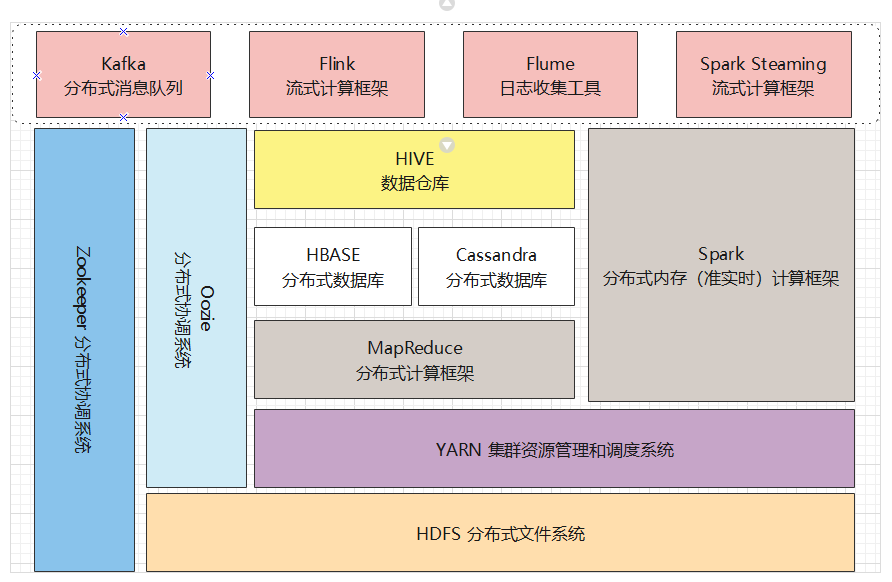
\includegraphics[width=0.99\linewidth]{figures/bigdata.png}
	\caption{大数据技术生态}
	\label{fig:bigdata}
\end{figure}


与此同时,GPU技术也取得了天翻地覆的变化,算力的快速发展解放了算法的双手,人工智能的各股力量开始逐渐汇集到以
BP算法为基础的深度神经网络的大旗下。
人们发现随着数据量的增加,复杂模型在小数据集上严重的过拟合现象得到了极大的缓解了,端到端的训练模式逐渐变成了主流算法。另外一些网络结构上的改进,例如\gls{CNN}、\gls{LSTM}、残差网络和注意力机制先后被提出来,计算机音视频处理能力快速从实验室研究走向工业应用。依托人脸识别功能的长足进步,从微信到支付宝,从火车站到医院,人脸识别被大量的应用起来。另外人工神经网络在音频信号处理和自然语言处理上的长足进步,催生出另一个重要的应用场景,这个场景就是智能助手。近几年,像小度在家、天猫精灵和小爱同学等大量硬件开始逐渐涌现,这些智能硬件希望通过重塑人机交互接口,掌控家庭控制中心,推动物联网技术普及。基于人工神经网络的自然语言处理技术,在传统搜索领域也开始逐步扎根并推陈出新,这几年依托语意向量化的向量检索技术开始逐步走进人们的视野。算法的智能化演进出现了多路并进,异彩纷呈的局面。

人工神经网络自然语言处理技术在这波算法智能化浪潮中可谓表现突出,从早期TextCNN从计算机视觉中汲取灵感,到后来Transformer技术对其他领域产生影响,以及Bert在近几年逐渐掀起人工智能革命的高潮,我们看到了人类对创造智能的巨大渴望。自然语言处理技术一直被认为是人工智能领域的明珠,因为自然语言是人类记录和传承知识和文化的重要手段,机器智能只有具备了从自然语言中吸取知识的能力,才有可能实现智能向智慧的转变。我相信在未来数十年的时间内,算法革命一定会从智能化向智慧化转变。所谓从智能化向智慧化的转变就是机器智能从认识事物向认知事物的转变。我比较相信自然语言处理技术特别是机器阅读理解能力将是这场转变中的重要技术基础。自然语言处理将不仅仅能够识别自然语言中的意图,而且能够逐步理解文本中的知识并具备知识抽取、推理和应用能力。我们已经逐渐开到了算法智能化浪潮的萌芽,商业投资的涨跌,将不会影响算法智能化浪潮
在曲折中成长壮大。


2020年岁在庚子,注定和历史上的其他庚子年一样不平凡,从岁初的大瘟疫,到岁中的洪灾和中美经贸摩擦,中国甚至世界的经济活力都遭遇了前所未有的巨大打击,互联网特别是AI技术更是备受冲击。很多公司都开始缩减开支,降低对算法的投入,自然语言处理技术作为目前人工智能领域研究和应用难度最高的技术也遭受了不小的冲击。不过我相信对自然语言技术的坚守就是对价值本身的坚守,前路漫漫但是前途光明,在算法的智能化甚至智慧化革命中,自然语言处理技术必将能勇挑重担,乘风破浪。我做出这种判断的依据主要有两个方面,第一、现有的神经网络自然语言处理技术面对传统规则系统已经展现出技术碾压的态势,其可用性和有效性已经逐步被工业界认可;第二、自然语言作为最广泛应用的信息载体,是互联网上最为广泛的数据,就像PageRank之前的网站孤岛一样,这些广泛存在的数据目前尚处在无法理解,无法认知甚至是没有应用依托的状态。然而可以肯定的是这些数据中包含着巨大的价值,人类数百年积累
的人文和科学领域的知识和文化都被蕴藏在这座尚未被挖掘出来的宝库中。自然语言处理技术作为撬开这座宝库的钥匙,必然是推动这轮信息技术革命后半程的攻坚力量。另外,
由于近些年的技术进步是非常惊人的,我们看到一些从业人员对其中的知识和成果的掌握是良莠不齐的。特别是这些年来自然语言处理技术出现井喷式发展,新技术层出不穷,人们甚至无暇系统性总结这些年的技术进步。我甚至注意到一些特别高阶的技术人才对最新的自然语言处理的技术成果都表现出不同程度的不明白或者不理解等现象。一方面为了能够帮助自己学习和进步,另一方面也是希望能够帮助大家梳理现有的研究成果,我萌生了撰写这本书的念头。希望能够用中国工程师熟悉的语言,将近几年自然语言处理领域的重要技术一一梳理总结,为奋战在互联网一线广大中国工程师提供一个入门的书籍,帮助他们找到入手方法,给他们提供一个近几年来自然语言处理技术研究的发展脉络图。为此本书从分词和词向量、语言模型、文本分类、预训练、语意信息检索机器翻译和机器阅读理解等若干技术角度进行展开,通过公式、图片和代码示例等手段逐步揭开自然语言处理的技术面纱。其中的每个章节我们或尝试从整体框架或尝试从具体研究入手,给大家展示自然语言处理的技术魅力。

最后由于本人的水平有限,这本书中不可避免会有一些错误或者不恰当的地方,希望大家多多包涵。这本书本身是我这些年的一些学习笔记,主要内容集中在自然语言处理领域。由于这些年自然语言处理技术的快速发展,本书不可能完整覆盖所有重要的内容,我只是从本人的知识和判断出发,梳理了这几年我认为重要的且比较有工业应用价值的研究成果,希望能起到抛转引玉的作用。


\chapter{自然语言处理技术的发展历史}
从第一个真正意义上具有使用价值的神经网络诞生到现在已经超过50年历史了,神经网络的发展史就是一部计算机的发展史。自然语言处理技术,作为人工智能领域的明珠,一直被认为是人类通往强人工智能的阶梯。人类文明历史中的所有知识储备都被以自然语言的形式存储在书籍或世代口口相传的文化传统中,理解和学习自然语言中蕴含的知识,是计算机真正能够实现意识觉醒的关键所在。因为掌握了知识,才能认识自己和客观世界,有了自我认识和对客观世界的认识,计算机才能够脱离工具属性,迈向强人工智能。自然语言处理技术是认知科学、计算机学甚至数学交叉的一门学科,其中计算机学和数学是手段,对自然语言的认知是目的。从自然语言发展的历史上看,可以泾渭分明的看到两个阶段:第一个阶段主要是以统计科学为基础的统计自然语言处理技术;第二个阶段主要是以人工神经网络为基础的人工神经网络自然语言处理技术。目前看自然语言处理技术已经发展到了第二阶段,人工神经网络对统计自然语言处理技术的决胜时刻
出现在2016年,谷歌大脑负责人Jeff Dean表示,他们用500行神经网络模型代码取代了50万行基于短语的统计机器翻译代码,并且效果惊人。这就像刘慈欣在《三体》里面介绍的二向箔攻击一样,神经网络实现了对统计机器翻译的降维打击。然而,从2001年Bengio 等人提出的第一个神经语言模型(\gls{NNLM})到神经网络机器翻译的高光时刻,神经网络自然语言处理技术已经默默发展了近15年的时间,而在此之前人们已经在统计自然语言处理领域默默耕耘了半个世纪。下面我们来梳理自然语言处理技术的发展脉络。

神经网络在自然语言处理领域的发展,主要有两个不时交叉的独立发展脉络,第一个脉络是自然语言的理解,第二个脉络是自然语言的生成。所谓自然语言的理解分为几个层面,第一个层面是对词汇的表示方法的探索;第二个层面是对句子中蕴含的意图的理解,以及基于句子语义的语言推理,包括句子之间的关系和语义信息检索等任务;第三个层面是对句子中的关键信息的提取,例如命名实体识别和时间抽取等任务。
所谓自然语言生成,目前的具有应用潜力的研究主要集中在两个层面,以机器翻译和文本摘要为代表的Seq2seq技术和基于神经网络语言模型的自然语言的自动生成技术。随着技术的发展人们渐渐的不满足于自然语言的理解和自然语言的生成,尝试让计算机通过阅读指定的文章来回答相关的问题,这就是非常著名的机器阅读理解问题,机器阅读理解是自然语言技术的一种综合应有,是自然语言处理技术的高级应用,甚至被认为人工智能从感知识别向认知理解转变的重要环节。我们这里没有把机器阅读理解归类到自然语言理解中,主要原因有两方面,一方面,机器阅读理解从本质上是一种知识提取工具,可以帮助抽取自然语言中的知识,所以着眼点是对自然语言的顶层认识;另一方面,机器阅读理解中自由问答同时涉及到比较复杂的自然语言理解和自然语言生成技术。当然这仅仅是一种分类的方法,这种分法可能不一定是完美的,我们这样分类的主要目的是为了突出自然语言发展的脉络。事实上,我们可以看到自然语言处理技术也经历从对自然语言
的理解到生成并产生从自然语言中进行知识提取的萌芽的过程,这个过程符合从简单到复杂的事物认识规律。智能和智慧的区别主要是是否能够主动提取并知识,目前的人工智能尚不具备这种智慧能力,但是人们已经开始尝试通过机器阅读理解技术提取自然语言中蕴含的知识,这是一种算法智能化的萌芽。

\section{自然语言理解的发展}
自然语言理解\gls{NLU}研究的主要内容是对自然语言的形式理解和有效的特征数学抽象方法。当计算机面对一段汉语文本的时候,首先需要掌握的技能就是如何将其分割成基本的表意单元,这就是我们常说的文本分词。在汉语中每个词而不是字都是具有一定语意的单元,因此文本分词就是一种语意的分割。传统的搜索引擎的工作原理就是通过计算Query和Doc的语意单元的重合程度来区分不同的Doc相对于同一个Query的语意相关性,TF-IDF和BM25就是这个时代最成功的算法,这两项技术和著名的PageRank算法是传统搜索引擎的基石,搜索引擎的出现解决了人们获取信息的问题,极大地拓展了每个人的知识边界,并引爆了第一次信息技术的浪潮。Yahoo、Google和Baidu等巨头企业都诞生于这个时代,第一批自然语言工程师也基本上诞生在这个时代。当时的工程师广泛使用的技术是统计自然语言处理,\gls{LDA}、\gls{LSA}和TextRank等复杂的统计自然语言处理技术都是那个时代
的产物。随着搜索引擎技术的发展,人们开始研究Query中蕴含意图的自动识别能力,最初人们将这个任务归结为文本分类任务,使用\gls{SVM}和Xgboost等统计分类技术来完成这个任务。由于\gls{SVM}和Xgboost等技术缺乏语义建模能力,因此其效果时好时坏;另外这些统计分类技术需要大量的特征工程,耗费人力物力,为此人们迫切的需要文本特征的合理数学表示。最初取得突破的技术是word2vec,这项技术通过简单的神经网络无监督学习方法,已经能够训练处表意良好的词向量。在此基础上,人们开始研发向量检索引擎用于语义检索,至此计算机界开启了神经网络自然语言处理研究的序幕。

得益于计算机视觉中图片分类技术的突破,人们开始尝试通过\gls{CNN}技术来实现文本特征的抽取,著名的文本分类算法TextCNN ,就是基于单层\gls{CNN}来实现文本特征抽取的。TextCNN的出现,极大鼓舞了人们对人工神经网络的信心。通过使用简单的端到端的神经网络,文本分类的准确度可以达到惊人的水平。随后的TextRCNN和\gls{SAN}等技术进一步拓展了文本特征抽象的算法工具。后来序列标注任务和序列生成任务的研究,都从不同的侧面验证了这种特征提取方法的有效性。文本分类任务后来在工业界的成功落地,也逐渐夯实了自然语言处理技术应用的基石。下面我们将从三个方面来介绍自然语言处理技术的发展历史,其中词汇的数学表示一节介绍分词技术和词向量技术;句子意图理解一节介绍文本分类和文本特征抽取;;句子中关键信息提取一节介绍序列标注任务极其应用。

\subsection{词汇的数学表示}
在现代汉语中,字并不是表意基本单元。汉语的基本表意单元是词,但是词的形式并不固定,一个词可能是一个字也可能是两个字甚至是更多的字。将一句话切分成其对应的表意基本单位序列我们称之为分词,分词技术在传统的搜索引擎中处于至关重要的地位,汉语搜索引擎的BM25算法就是基于词汇来做的。最初人们使用的是词典匹配的方法,这些都属于启发式的分词算法,后来随着\gls{HMM}和\gls{CRF}在其他领域逐渐显现出威力,人们发现将分词任务建模成\gls{HMM}或者\gls{CRF}模型效果非常好,例如广泛试用的jieba分词模型的分词准确率超过了$0.80$。后来随着序列标注技术的进一步发展,Bi\gls{LSTM}、\gls{IDCNN}甚至\gls{BERT}融合\gls{CRF}等技术的出现,基本上将中文分词任务的分词准确度,推高到了$0.95$甚至更高,至此分词问题基本上宣告解决。

然而,如何将词汇转换成可计算的形式呢?有了词汇的数学表示我们就可以计算近义词甚至反义词,甚至进行敏感词联想和发现等等任务。21世纪初人们依然在广泛使用一种非常原始的词汇表示法——one-hot。所谓one-hot就是一个长度为$n$的向量,其中只有一个位置是$1$,其他地方都是$0$。为了避免冲突$n$
一般等于词典的大小,one-hot向量值为$1$的位置下标等于词汇在词表中的ID。这种原始表示法只能进行非常有限的语义运算,无法刻画词汇的真实含义。2013年word2vec的出现,彻底扭转了词汇数学表示无法刻画语义的局面,通过简单的一个浅层网络,经过梯度下降拟合之后计算出来的词向量具备了惊人的语义表达能力。例如利用这种技术训练出来的词向量进行相似词推理,可以发现“刘德华”的近义词是“刘天王”,“自然语言处理”的近义词是“自然语言理解”。后来人们在word2vec的基础上通过引入\gls{LDA}等相关技术,进一步推动了词汇的数学表示形式的发展,以至于目前词向量已经成为自然语言处理领域的基础技术之一,在文本分类、序列标注和机器翻译等领域都在发挥基石性作用。图\ref{fig:history1.png} 是腾讯AILAB通过\gls{LDA}和word2vec融合训练出来的词向量联想的近义词例子。
\begin{figure}[htbp]
\begin{center}
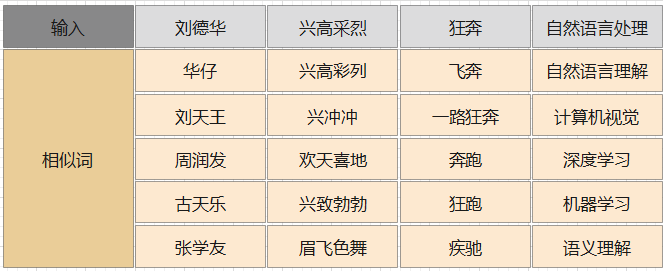
\includegraphics[width=5.5in]{figures/history1.png}
\caption{词向量的近义词联想} \label{fig:history1.png}
\end{center}
\end{figure}

\subsection{句子的意图理解和语义推理}
\subsubsection{句子意图理解}
句子意图理解,就是给定一个句子,判断这个句子表述的语义中蕴含的意图。在搜索引擎中给定一个搜索Query,判断这个句子所属的搜索领域,然后到对应的垂直检索引擎中抓取结果,就属于句子意图理解的一个重要应用。搜索引擎的聚合结果背后的关键技术就是句子的意图识别。句子意图识别的另一个重要的应用是在对话领域对句子的对话领域进行对话意图识别,例如在自动订票系统中,识别订票的类型是订飞机票还是火车票就属于这类技术的应用。

句子意图理解可以建模成文本的分类技术,最初人们使用最多是$\gls{SVM}$和$xgboost$等浅层模型,人们发现这种技术需要大量的特征工程,对不同的任务,需要单独设计特征,而且其泛化性能比较弱。文本分类技术的曙光出现在2014年,Yoon Kim 在当年的EMNLP中的一篇论文中指出可以像图片分类一样使用\gls{CNN}来解决文本分类任务,而且其效果非常好。在计算机看来经过Embedding处理后的文本和一
张单通道的图片并无本质不同,因此彼时在图片分类领域已经大获成功的\gls{CNN}技术,用于文本分类任务的尝试出现,应该是一种历史的必然。至此文本分类技术正式宣告进入神经网络时代,这项研究是自然语言处理技术的里程碑式的事件,从此,基于人工神经网络的语义建模,走进了人们的视野。人们开始尝试将在图片分类领域取得成功的深度卷积神经网络应用到文本分类领域,例如有些研究者提出了\gls{VDCNN},这种技术就是尝试将在图片分类领域取得突破的深度残差神经网络应用于文本分类领域,文章设计一个高达49层的深度残差神经网络,并取得比很好的效果。

文本分类的另一条发展脉络是循环神经网络,循环神经网络特别是\gls{LSTM}在语音识别领域最早出现突破。自然语言同样是一种具有序列特征的信号,那么能不能将循环神经网络应用于文本分类领域呢?人们发现,在文本分类领域,\gls{LSTM}网络甚至比\gls{CNN}的效果更优秀。大概也在2014年前后,循环神经网络在机器翻译领域迎来高光时刻。人们开始发现用循环神经网络进行自然语言的语义建模是非常有效的,至此自然语言领域开始了\gls{CNN}和\gls{RNN} 的竟跑模式,我们在表\ref{tab:rnncnnhistory}中简单罗列了人们在\gls{CNN}和\gls{RNN}领域的一些代表性成果。
\begin{table} [h]
	    \begin{center}
    \begin{tabular}{p{50pt}p{150pt}p{160pt}}  % 10cm 減去前兩個欄位寬度後,剩下的通通給
        \hline    
        领域&\gls{RNN}&\gls{CNN}\\
        \hline    
        语言模型& \gls{RNN}语言模型\gls{RNNLM} & 门控\gls{CNN}语言模型\gls{CNNLM} \\
        \hline   
        词向量 & 上下文词向量ELMo & - \\
        \hline
        序列标注 & BiLSTM+\gls{CRF} & \gls{IDCNN}+\gls{CRF} \\
        \hline
        文本分类 &TextRCNN & TextCNN、TextRCNN、charCNN和\gls{VDCNN} \\
        \hline
        句对分类& ESIM & ABCNN \\
        \hline
        机器翻译 & \gls{RNN}+LuongAttention、\gls{GRU}+BahdanauAttention & 门控CNN+Multi-step Attention \\
        \hline
    \end{tabular}
    \caption{RNN和CNN在NLP领域的研究成果}  \label{tab:rnncnnhistory}
    \end{center}
\end{table}  

目前已经日渐明朗的事实是,循环神经网络(\gls{RNN})和卷积神经网络(\gls{CNN})都是非常有效的文本特征提取手段而被广泛应用到诸多领域,不过\gls{CNN}和\gls{RNN}技术也在这场竞拍中迎来巨大的挑战者。这个挑战者就是基于自注意力的预训练模型(\gls{SAN}),自注意力预训练技术是通过两阶段的训练,来把海量语料中的语义信息融合到下游任务中去,从而改进模型的表现。预训练机制的第一个步骤,一般可以被认为是动态词向量,可以理解为将词语的数学表示和其对应的上下文联系起来。预训练机制的第二个步骤,一般是对动态词向量的一种适配微调的过程,通常学习率比较低。目前\gls{RNN}、\gls{CNN}和\gls{SAN}已经成为主流的三种文本特征抽取工具,受到了广泛的关注。

\subsubsection{语义推理}
判断两个句子的关系,一直是广受关注的自然语言处理任务。在桌面搜素引擎流行的时代,人们解决的核心问题就是给定一个Query从海量的WEB页面中找语义最相关若干页面。为了解决这个问题,最初人们使用的是统计学的手段,最著名的方法是BM25和tf-idf等。这些方法根据词汇的词频信息来建立Query和Doc的统计联系,这些方法虽然不能很好的建立语义联系,但是已经在很大程度上,满足了人们的需要。这种统计搜素技术甚至催生出一些世界级的大公司,例如雅虎和谷歌。然而随着人工神经网络在语义建模领域的快速进步,人们开始尝试建模句子内部的语义联系。

早期神经网络语义搜索领域最具代表性的研究是孪生双塔结构,这种网络用两个共享参数的孪生网络结构来同步建模Query和Doc,并在Query和Doc建模完成后,建模两者的相似度。这种网络结构的文本表示层,最初使用多层感知机,随着句子语义表示的发展,人们先后将\gls{CNN}、\gls{RNN}甚至预训练的自注意力网络应用于句子的语义表示层,以改进模型的表现。这种孪生网络结构通常被称为BiEncoder。但是后来人们发现在建模句子语义的时候,如果能够一开始就建模两个句子的语义关系,而不是在最后构建损失的时候构建语义关系,可以明显改进句子语义建模的效果。这方面比较有影响力的研究是ABCNN和ESIM,这两种网络分别将交互注意力机制引入\gls{CNN}和\gls{RNN}从而改进了句子语义建模的效果。后来人们发现直接使用预训练和自注意力机制网络能够更好的建模语句之间的联系,特别是\gls{BERT}的出现,把句子语义建模推到非常高的水平。这种融合交互注意力的语义关机建模手段
通常被称为CrossEncoder。

BiEncoder和CrossEncoder从语义关系建模的角度看,前者明显劣于后者;但是从召回速度的角度看,前者明显优于后者。BiEncoder一方面可以预先缓存Doc的表示向量到向量检索引擎中去的,因此避免了重复计算;另一方面BiEncoder可以和向量检索引擎结合从而处理海量Doc的快速召回。这些特点帮助BiEncoder赢得了工业领域的青睐,成为后来经典的召回-排序两阶段框架的召回部分的重要算法。CrossEncoder由于其良好的语义建模能力,成为召回-排序框架排序阶段的最成功算法。这种两阶段框架后来成为智能对话甚至商品推荐等领域的标准框架。

\subsection{句子中的关键信息的提取}

在自然语言的任务型人机交互领域,人们通常将一条自然语言抽象成一条指令,一条指令通常会携带若干参数,例如播放音乐的指令,通常需要一个参数就是要播放的音乐的名称;而订购机票的指令,通常会有一个参数就是订票的时间和往返城市。人们常常通过一个文本分类器将可执行的指令识别出来,然后利用句子信息提取技术提取执行指令所需要的的参数。通常句子关键信息提取技术有两种基本分方法:第一种基于序列标注,第二种基于序列生成。
\subsubsection{序列标注法}
使用序列标注的方法解决句子中关键信息提取时,人们最初使用的是统计学的方法,最常见的两种算法是:隐马尔可夫过程\gls{HMM}和条件随机场\gls{CRF}。隐马尔可夫过程是生成模型,虽然其不需要太多的特征工程,但是效果不及条件随机场。条件随机场就是在人工神经网络发展的早期最为流行的解决序列标注问题的方法,这种方法的效果非常好,但是依赖大量的特征工程投入,并且数学理论复杂,因此慢慢被后来兴起的人工神经网络所替代。2015年的时候,Baidu公司的研究人员,提出用双向\gls{LSTM}来替代条件随机场中的特征抽取工作,在命名实体识别领域可以取得非常好的效果。至此人们开始关注人工神经网络在序列标注领域的应用。2017年的时候,有研究者汇报使用膨胀卷积可以高效快速完成序列标注任务。这种算法在训练速度和推理速度都更快的前提取得了和BiLSTM-\gls{CRF}同等的效果。另外,有部分研究者把主要集中在结合意图分类和序列标注任务的方向上,借助意图和实体的关联性提高模型的效果。在这个方向上,人们先后尝试了孪生网络、门控\gls{RNN}和\gls{BERT}等多种算法。由于任务型聊天和IOT的结合,逐渐显现出商业价值,因此这个领域的研究可谓异彩纷呈。我们会在后续的章节中详细介绍。
\subsubsection{序列生成法}
序列生成方法是句子信息提取的高级形式,模型通过理解输入的文本,经过自己的处理加工,按照自己的理解把句子中需要的关键信息提取出来。得益于Seq2seq技术在机器翻译领域的巨大成功,人们开始尝试将序列生成技术应用于句子信息提取工作,这方面早期的代表性研究是Liu Bing 等人提出的在传统seq2seq中引入对齐机制和注意力机制来完成序列标注。这种方法思路非常新颖,是值得关注的一个研究方向,在IOT场景中可能有很大的应用前景。
\section{自然语言生成的发展}
自然语言生成技术最为人熟知的技术是\gls{GPT}-x和Transformer,这两项技术属于两种不同的句子生成方法,前者是基于语言模型的自动句子生成技术;后者是基于Seq2Seq的文本生辰技术。所谓Seq2seq就是指给定一个源语句,网络预测目的语句的过程。常见的应用有机器翻译、文本摘要和对话生成技术,分别用于完成语义的形式转换、文本的精简和语义的联想。我们将分两个方面来极少自然语言生成技术的发展。
\subsection{语言模型和自动造句技术}
在自然语言处理技术发展的早期,人们的一个重要的研究方向是如何评判一个句子是不是通顺的,一个常见的方式就是计算其各个词按照句子中的顺序出现的概率:
$$
P(w_1,w_2,\cdots,w_n) = \prod_{i=1}^{n}{P(w_i|w_{<i})}
$$
其中$P(w_i|w_{<i})$表示在语料库中,出现前若干词一次出现$w_1,w_2,\cdots,w_{i-1}$的条件下,第$i$个词是$w_i$的概率。事实上这个概率越下,人们读到这个句子的时候就越觉得不通顺,越困惑,为此人们通常使用困惑度来衡量一个句子的好坏。
$$
PPL(w_1,w_2,\cdots,w_n) = -\frac{\sum_{i=1}^{n}log(P(w_i|w_{<i}))}{n}
$$
早在2001年,Bengio和他的研究伙伴就开始使用神经网络来计算一个给定语料库的$P(w_i|w_{<i})$,遗憾的是,他们并没有建模句子的顺序。后来Mikolov等人在2010年前后开始使用\gls{RNN}来建模句子的表达顺序,以更精准的刻画$P(w_i|w_{<i})$,当然后来又有\gls{CNN}网络来解决同样的问题。
$P(w_i|w_{<i})$的计算问题通常被称为语言模型问题,甚至后来人们发现自注意力机制也可以来构建语言模型,而且效果惊人。

语言模型一方面能够评价一个句子的困惑度,另一方面也可以用来造句子。例如给定一个前$k$个词,语言模型可以将其扩展到一个给定的长度,并保证句子尽量通顺。这个构造过程可以使用动态算法来穷举所有可能,也可以使用BeamSearch来近似动态穷举算法,甚至可以使用GreedySearch来贪心构造句子。很多自然语言的研究人员不清楚这三者的区别和联系。我们这里简单介绍一下这三者的区别和联系,我们在构造长度为$k$的句子前缀的时候,最佳的选择是使得$P(w_{<k})$最大的序列,可以构建如下的递推关系
$$
P(w_{<{k}}) =\max_{\widetilde{w}_{<{k-1}}}\{P(\widetilde{w}_{<{k-1}})P(w_k|\widetilde{w}_{<{k-1}})\} 
$$
如果我们通过动态规划解决$P(w_{<k})$问题,那么就是使用穷举法。由于上述的计算规模非常巨大,需要近似算法,具体的计算方法如下
$$
\begin{aligned}
P(w_{<{k}}) &=\max_{\widetilde{w}_{<{k-1}}\in A_{k-1}}\{P(\widetilde{w}_{<{k-1}})P(w_k|\widetilde{w}_{<{k-1}})\} \\
A_{k-1} &=top\_m\_of(P(w_{<K}))\\
\end{aligned}
$$
其中$top\_m\_of(P(w_{<k}))$表示$P(w_{<K})$中取值最大的$m$个序列。这种计算方法被称为BeamSearch,如果$m$取值为1,那么BeamSearch就退化成GreedySearch。


现在广泛流行的\gls{NLP}算法游戏,例如藏头诗就是基于这种技术的一个应用。

\subsection{序列到序列技术的发展}
在西方语言文字发展的历史中最早的语言形式是苏美尔人创造的象形文字,后来象形文字逐渐演化成楔形文字,之后被腓尼基人改造成表音文字,最后经过古希腊和古罗马人的继承和发扬形成了的拉丁文,而拉丁文可以被看成是现在西方主流语言之母。在东方语言文字发展的历史中,象形文字并没有演变成表音文字,依然是一种象形文字的抽象简化形式。目前世界上并存着大量各种形式的语言文字,如何让计算机实现不同形式的语言之间的同义转换,一直是自然语言处理技术的核心问题。最初人们使用的技术是笨重的统计机器翻译系统,一个商用的统计机器翻译系统,需要大约数十万甚至数百万行的代码。但是随着神经网络在语义建模领域的成功,有研究者开始使用编码器到解码器的框架,简单来说就是先利用\gls{CNN} 或者\gls{RNN}进行源语言的语义建模,然后利用建模结果来指导解码器进行造句。其中造句的方法主要包括GreedySearch 和BeamSearch等。这类研究由于其可以根据变长的输入来构造一个
变长的输出,因此一般被称为序列到序列。

最初的方法人们会将源句子的表示浓缩成一个向量,忽略源语言的序列特征。由于注意力机制在计算机视觉领域的快速发展,人们发现利用注意力机制,可以更充分利用源语言的结构、语法和语义信息。到2016年的时候,Google宣布其基于神经网络的计算机翻译系统,开始超越传统的基于统计的机器翻译系统,序列到序列的研究开始迎来了第一个高峰。2018年的时候Google公司的研究人员发表了一篇文章,文章声称"Attention is all your need"。这篇文章以一种非常豪迈的姿态,把序列到序列的研究推向了第二个高峰。他们的研究中提出的模型被称为Transformer,事实上,这种豪迈的姿态是有充分的实力支撑,Transformer 一举刷新所有自然语言翻译的记录,而且提出了一种完全基于自注意力的语义建模方法。结合预训练技术和掩码语言模型,这种基于自注意力机制的语义建模方法,开始引爆正自然语言研究和应用领域,甚至有逐渐成为引领机器学习革命的
双引擎之一的趋势。另外的一个引擎公认的是是计算机视觉领域的突破。2019年的\gls{BERT}技术,就是发端于Transformer的基础技术,\gls{BERT}一经面世就以一种碾压姿态,刷爆了GLUE-benchmark的所有11个任务。

由于序列到序列建模方式在机器翻译领域的成功,人们开始注意到,其实生成式问答领域也可以建模成序列到序列任务,甚至推荐系统中也可以应用相关的技术思想。

\section{机器阅读理解}
\begin{figure}[htbp]
\begin{center}
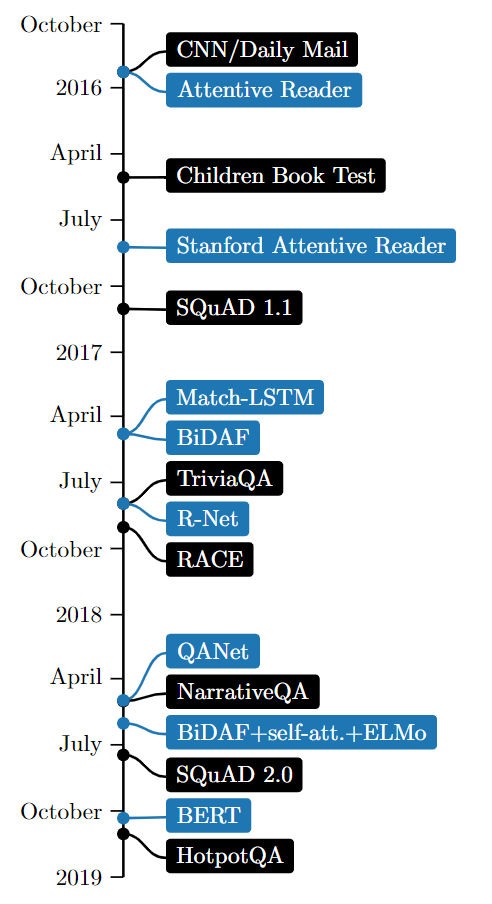
\includegraphics[width=4.0in]{figures/mrc1.png}
\caption{机器阅读理解的发展时间线} \label{fig:mrc1}
\end{center}
\end{figure}
机器阅读理解技术一直被认为是自然语言处理最复杂和最具挑战性的任务,机器阅读理解的目标是从语料中学习知识,并能够通过学到的知识回答相关的问题。目前被学术界广泛研究的问题形式主要有四种——完形填空、多项选择、答案片段抽取和自由问答。完形填空是学生语言能力考试中的一种常见形式,通常考题会将文本中一些关键信息实体从原始文本中挖去,然后然学生通过对原始文本的上下文理解来推测挖去的实体,从而考察学生对文本的理解能力。2016年在机器阅读领域,具有开创意义的研究——Attentive Reader、Impatient Reader模型就是来解决完型填空问题的,这项研究是基于BiLSTM和Attention机制来实现的。多项选择题的形式类似于英语考试中的阅读理解(选择题),给定一篇文章,通过阅读并理解文章(Passage),针对提出的问题(Question)从若干个选项中选择正确的答案(Answers)。这种类型的阅读理解
答案并不一定在文章中,需要有对原始文本的语意理解才能准确从备选答案中选出正确答案。比较有代表意义的研究是Dual Co-Matching Network,这项研究是上海交通大学提出的。机器阅读理解的另一个重要方向抽取,抽取式机器阅读理解,是要在文档中定位问题的答案。模型输入是文章[Passage]、问题[Question],模型输出是$[start\_idx,end\_idx]$,$ start\_idx,end\_idx \in [ 0, len(passage) ]$,在这方面最著名的模型是BiDAF和matchLSTM 等模型。自由问答是四种任务中最难的一种形式,是极具挑战的阅读理解形式,目前学术研究尚在萌芽中。如图\ref{fig:mrc1}所示,我们简单梳理了机器阅读理解的整体发展历史时间线。


\chapter{人工神经网络基础知识}
本章我们将介绍一些人工神经网络的基础知识,首先我们会介绍常见卷积神经网络、循环神经网络和残差网络等基本网络组件,以希望大家能够了解常见神经网络关键组件的运算原理;之后我们会介绍基本的优化器相关知识;最后我们会介绍一些正则化的方法、防止过拟合的方法和规范化相关的知识,以希望大家能够将神经网络的能力发挥到最大。一般在自然语言处理领域一句话通常可以表示成一个实数矩阵,具体的做法是首先为每个词分配一个整数ID,然后每个整数ID对应一个随机初始化的向量,这样一句话就可以表示成一组向量组成的矩阵。为了方便,我们假定句子的长度是$n$,每个随机初始化的词向量的维数是$h$,句子的实数矩阵表示为$S=\{s_{i,j}|i=1,2,\cdots,n;j=1,2,\cdots,h\} $。

\section{常见的网络组件}
\subsection{基本神经元和全连接层}
\subsubsection{感知器与全连接层}
感知器是一种非常古老的线性分类器,可以快速解决线性可分的样本中的分类问题。这个算法提出到现在已经有超过70年的历史了,算法非常简单,对于输入的样本特征进行加权求和,之后通过一个激活函数得到模型的输出。通过简单的梯度下降算法,感知器能够快速收敛。假定输入的样本特征为$X=[x_1,x_2,\cdots,x_n],x_i\in \mathbb{R}$,那么输出的结果$Y$等于
$$
Y=f(XW^T+b)
$$
其中$W=[w_1,w_2,\cdots,w_n]$是权重向量,$b$是偏置标量,在特定的任务中,这两个参数需要通过梯度下降法来习得。$f$是激活函数,可以是线性函数也可以是非线性函数。如$W$是一个$k\times n$的实数矩阵$W \in \mathbb{R}^{n\times k}$,且$b$是一个$1\times k$的实数矩阵$b \in \mathbb{R}^{1 \times k}$,那么上述感知器就变成了一个全连接层,实现了特征从一个$n$维空间到$k$维空间的变换。
需要注意的是全连接层具有非常强大的拟合能力,非常容易发生过拟合的现象,一般要加dropout等正则项。

\subsection{卷积神经网络及其变体}
\subsubsection{经典卷积}
卷积神经网络是自然语言处理领域的重要结构,然而不同计算机视觉中的卷积神经网络,在自然语言处理领域,通常卷积核只在一个维度进行滑动,以抽取n-gram特征。卷积神经网络通常会定义若干个卷积核,在自然语言处理领域,一般一个卷积核可以定义为一个可学习的矩阵$W_i \in \mathbb{R}^{k \times h}$,卷积神经网络可以理解为将卷积核理解为一个滑动窗口,在句子实数矩阵上滑动求和,得到一组实数$F_i=[f_{i,1},f_{i,2},\cdots,f_{i,n-k+1}]$。这组实数序列表示一个卷积核抽取到的一个文本特征,通常的神经网络会抽取不止一个文本特征,如果要抽取$m$个文本特征通常需要$m$个可学习的卷积核$W=[W_i|i=1,2,\cdots,m;W_i\in \mathbb{R}^{n \times h}]$,在文本实数矩阵上分别执行滑动求和操作,得到$m$组特征向量
组成的矩阵$F=[F_1,F_2,\cdots,F_m]^T$,这个矩阵通常被称为特征矩阵。
$$
f_{i,j}=\sum{S[j:j+k;:]W_i^T}
$$
\begin{figure}[htbp]
\begin{center}
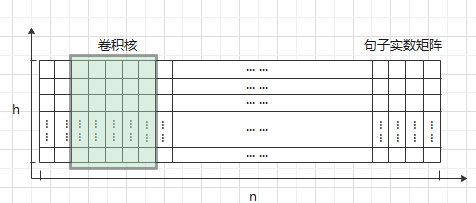
\includegraphics[width=5.0in]{figures/cnn1.png}
\caption{卷积核的滑动过程}
\label{fig:cnn1}
\end{center}
\end{figure}
为了方便我们把卷积操作定义为$F=\mathbb{\chi}(S;W)$。
另外需要强调的是,如果在句子矩阵的前后补上一定数量的零,并且令$m=h$,可实现特征矩阵和句子实数矩阵的尺寸相同,这是使用卷积神经网络实现序列标注任务的一个技巧。
\subsubsection{门控卷积}
在循环神经网络中,增加门控机制的\gls{LSTM}和\gls{GRU}都取得了巨大的成功,所以很自然人们想到了在卷积神经网络中增加门控机制,来学习如何挑选特征。由于卷积神经网络没有细胞状态,不存在梯度爆炸或者消失的现象,因此门控卷积神经网络没有设计复杂的遗忘门,仅仅设计了一个输入门,控制信息的流动,学习如何挑选对任务更有用的特征。门控卷积简单来说就是使用一对平行的卷积核来抽取一对平行的特征矩阵,然后将其中一个特征矩阵经过$sigmoid$函数变换到$[0,1]$空间上和原始矩阵按位置相乘,得到最后的输出:
$$
F=\mathbb{\chi}(S;W) \otimes sigmoid(\mathbb{\chi}(S;V))
$$
在自然语言处理领域,门控卷积最早被汇报用于解决语言模型的训练问题,后来又被用于机器翻译领域。门控卷积在这些训练数据庞大,需要较长训练时间的神经网络训练任务中,由于其出色的并行能力,和有竞争力的效果,一度成为人们研究的焦点。
\begin{figure}[htbp]
\begin{center}
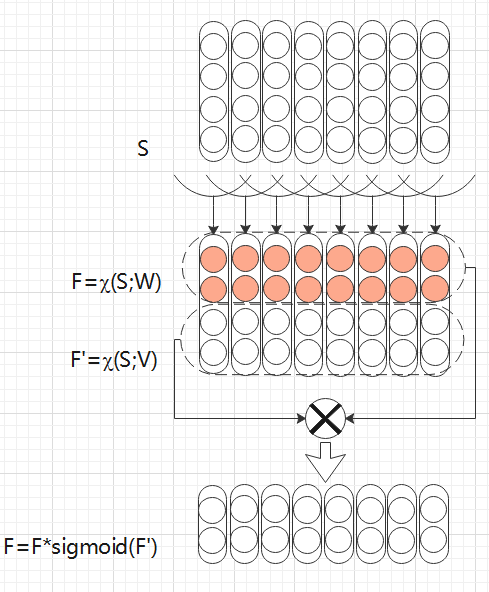
\includegraphics[width=5.0in]{figures/gcnn1.png}
\caption{门控卷积神经网络的计算流程}
\label{fig:gcnn1}
\end{center}
\end{figure}
\subsubsection{膨胀卷积}
\begin{figure}[htbp]
\centering
\subfigure[A.原始卷积]{
\begin{minipage}[t]{0.70\textwidth}
\centering
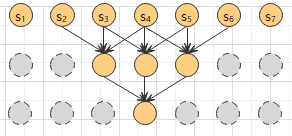
\includegraphics[width=4.0in]{dcnn1.png}
\end{minipage}
}
\subfigure[B.膨胀卷积]{
\begin{minipage}[t]{0.70\textwidth}
\centering
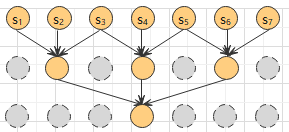
\includegraphics[width=4.0in]{dcnn2.png}
\end{minipage}
}
\caption{原始卷积和膨胀卷积}
\end{figure}
膨胀卷积最早被人们用来解决序列标注问题中长距离依赖问题。为了增加感受野的宽度,人们通常会层叠很多层的卷积。我们将卷积核写成列向量形式$W_i=[W_{i,1}^T,W_{i,2}^T,\cdots,W_{i,k}^T]$,并定义一个$h$维零向量$O$。那么卷积核核层数的关系如表\ref{tab:idcnn}所示。
\begin{table} [h]
    \caption{膨胀卷积}
	\label{tab:idcnn}
	\centering
    \begin{tabular}{l|c}  % 10cm 減去前兩個欄位寬度後,剩下的通通給  
        \hline    
        层序号&卷积核\\
        \hline    
        1&$W_i^{(1)}=[W_{i,1}^T,W_{i,2}^T,\cdots,W_{i,k}^T]$\\
        \hline                      % 第三欄位使用,文字超出的部份會自動折行  
        2&$W_i^{(2)}=[O,W_{i,1}^T,O,W_{i,2}^T,\cdots,W_{i,k}^T,O]$ \\  
        \hline  
        3&$W_i^{(2)}=[O,O,O,W_{i,1}^T,O,O,O,W_{i,2}^T,\cdots,W_{i,k}^T,O,O,O]$ \\  
        \hline
        $\cdots$ & $\cdots$ \\
        \hline
        n&$W_i^{(n)}=[\underbrace{O,\cdots,O,W_{i,1}^T}_{2^{n-1}},
        \underbrace{O,\cdots,O,W_{i,2}^T}_{2^{n-1}},
        \cdots,
        \underbrace{O,\cdots,O,W_{i,k}^T}_{2^{n-1}},
        \underbrace{O,\cdots,O}_{2^{n-1}-1}]$ \\  
        \hline
    \end{tabular}
\end{table}  

\subsubsection{卷积中的池化}
在卷积层的后面常常会有一个池化层,用于将特征图进行压缩,避免参数过多造成过拟合。常见的池化有2种:一种是最大池化,另一种是平均池化。Pooling 通常会在特征图的一个滑动矩形窗口中进行求最大值或者求平均操作。通常最大池化用于提取特征图的细节特征,而平均池化相当于一种平滑,用于提取特征图的低频统计特征。图\ref{fig:pooling1}所示就是一个例子。
\begin{figure}[htbp]
\begin{center}
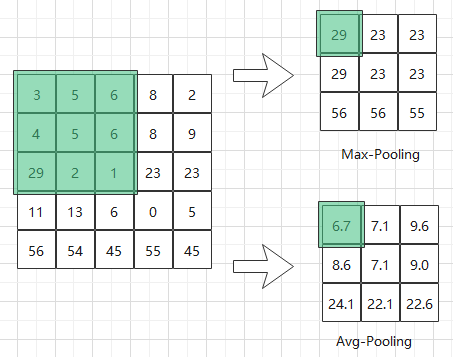
\includegraphics[width=5.0in]{figures/pooling1.png}
\caption{卷积神经网络中的两种池化}\label{fig:pooling1}
\end{center}
\end{figure}
\subsection{循环神经网络及其变体}
循环神经网络通常用来建模序列信息,除了输入,循环神经网络还有一个隐状态,用于建立历史输入对当前输入的影响。对于$i$时刻
$$
\begin{aligned}
H_i&=f(X_iU^T+H_{i-1}W^T)\\
Y_i&=H_i
\end{aligned}
$$
其中$f(x)$是激活函数,可以是$tanh$、$sigmoid$或者$relu$等。
\begin{figure}[htbp]
\begin{center}
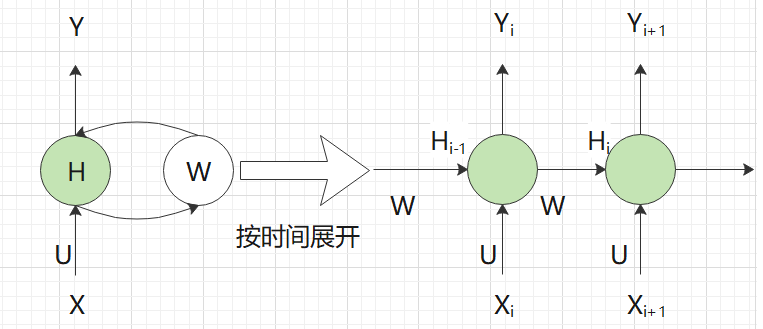
\includegraphics[width=5.5in]{figures/rnn2.png}
\caption{循环神经网络}
\label{default}
\end{center}
\end{figure}

循环神经网络的梯度求解涉及到一种称为BPTT的算法,但是这种算法会造成梯度消失或者膨胀。
$$
\begin{aligned}
\frac{\partial{Y_i}}{\partial{W^T}}
&=\frac{\partial{f(X_iU^T+H_{i-1}W^T)}}{\partial{W}}\\
&=f'(X_iU^T+H_{i-1}W^T) H_{i-1}\frac{\partial{H_{i-1}}}{\partial{W^T}}\\
&=f'(X_iU^T+H_{i-1}W^T)H_{i-1} \frac{\partial{Y_{i-1}}}{\partial{W^T}} 
\end{aligned}
$$
为了方便我们记$f'_{i}(W)=f'(X_iU^T+H_{i-1}W^T)$,那么我们得到
$$
\begin{aligned}
\frac{\partial{Y_i}}{\partial{W^T}}&=f'_{i}(W)H_{i-1}\frac{\partial{Y_{i-1}}}{\partial{W^T}}\\
&=f'_{i}(W)H_{i-1}f'_{i-1}(W)H_{i-2}\cdots f'_{2}(W)H_1\frac{\partial{Y_{1}}}{\partial{W^T}}\\
&=\prod_{j=i,i-1,\cdots,1}f'_{j}(W)H_{j-1}\frac{\partial{Y_{1}}}{\partial{W^T}}
\end{aligned}
$$
在$i$时刻,$Y_i$对于$W$的梯度是$\frac{\partial{Y_{1}}}{\partial{W^T}}$乘以一连串的因子,在训练的过程中,容易引发不稳定,这就是梯度的消失或者膨胀,或者换个角度讲,这种模型难以建立长程的依赖。人们后来提出的\gls{LSTM}和\gls{GRU},通过学习信息的保留和遗忘机制,缓解了上述问题。需要强调的是只是缓解,并没有根除,所以在很多时候还需要梯度裁剪,防止出现梯度爆炸。
\subsubsection{LSTM长短记忆网络}
长短记忆网络是人们对\gls{RNN}基本单元的改造,通过添加输入门和遗忘门,来缓解梯队的消失或者膨胀问题。长短记忆网络存在一个细胞状态$C_i$,隐层状态依赖前一时刻的隐层状态$C_{i-1}$,长短记忆网络首先要确定要从前一个时刻保留什么,这个门被称为遗忘门,
$$
f=\sigma([Y_{i-1};X_i]W_f^T+b_f)
$$
接着需要确定细胞状态需要更新什么,这个门被称为更新门,
$$
\begin{aligned}
g&=\sigma([Y_{i-1};X_i]W_g^T+b_g)\\
c&=tanh([Y_{i-1};X_i]W_c^T+b_c)
\end{aligned}
$$
细胞新的状态值等于遗忘掉的内容加上更新的内容,这样我们就可以知道如何更新细胞状态了
$$
C_{i}=f\otimes C_{i-1} + g \otimes c
$$
最后是根据新的细胞状态决定输出什么,这个门被称为输出门,
$$
\begin{aligned}
o&=\sigma([Y_{i-1};X_i]W_o^T+b_o) \\
Y_{i}&=o\otimes tanh(C_i)
\end{aligned}
$$
\begin{figure}[htbp]
\begin{center}
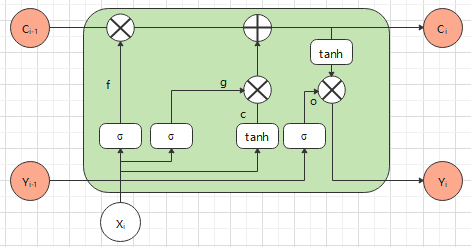
\includegraphics[width=5.5in]{figures/lstm1.png}
\caption{长短记忆网络}
\label{fig:lstm1}
\end{center}
\end{figure}
由于\gls{LSTM}比较复杂,在某些需要时候,需要较为简单的模型,因此\gls{LSTM}的简化模型\gls{GRU}就出现了。事实上,根据本人多年的经验,\gls{LSTM}和\gls{GRU}在效果上没有特别大的区别。
\subsubsection{单向和双向循环神经网络}
人们在实践中发现,对给定的句子,从左到右按照自然顺序执行循环神经网络对句子的语义建模效果,通常比从右往左按照自然顺序的逆序执行循环神经网络要差。那么能不能两个方向都执行一下,然后将结果拼起来,效果如何呢?事实上在很多时候这种双向执行的循环神经网络的语义建模效果要好于单向的。在命名实体识别和神经网络机器翻译中,人们已经证实了这个结果。假定从左到右执行后,句子的语意特征为$[\overrightarrow{h_1},\overrightarrow{h_2},\cdots,\overrightarrow{h_n}]$;从右到左执行后,句子的语意特征为$[\overleftarrow{h_1},\overleftarrow{h_2},\cdots,\overleftarrow{h_n}]$,那么句子的双向循环神经网络的语意表示为
$$[(\overleftarrow{h_i};\overrightarrow{h_i})|i=1,2,\cdots,n]$$
\begin{figure}[htbp]
\begin{center}
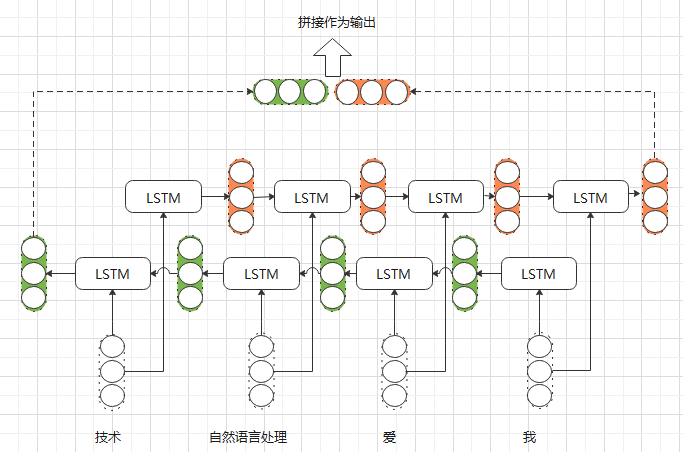
\includegraphics[width=5.5in]{figures/bilstm1.png}
\caption{双向循环神经网络}
\label{fig:bilstm1}
\end{center}
\end{figure}
\subsection{残差网络}
人们在深度学习的研究中,发现了一种非常难以理解的现象。概括来说就是随着网络层数的增加,模型的表现先是逐渐变好,然后又逐渐变差。这种当网络的层数增加到一定的高度后,模型的错误率突然变高的现象,被称为神经网络的退化现象。这种网络退化现象,比较违背人们的直觉,因此和梯度的消失或者爆炸现象一起被不少人认为是笼罩在人工智能领域的两朵乌云。为了克服这两个问题,人们尝试了一种跳线连接的方式,这种方式就是残差网络。假定网络第$l-1$层的输出是$X^{l-1}$,第$l$层网络可以表示成$X^l=\mathcal{F}(X^{l-1})$。如果我们为这个网络层引入残差连接,那么$X^l=\mathcal{F}(X^{l-1})+X^{l-1}$。这好比在损失层与任何网络层之间引入了一个跳线连接,增强了损失传递的到下层的效率,缓解了梯度从高层向低层反向传播的过程中,低层的梯度和损失函数的关联度下降严重的现象。
在\gls{NLP}中,人们已经证明在多层\gls{LSTM}中引入残差连接能够帮助提升\gls{RNN}翻译系统的效果;另外,Transformer和\gls{BERT}的网络结构也引入了残差连接。
\begin{figure}[ht]
\begin{center}
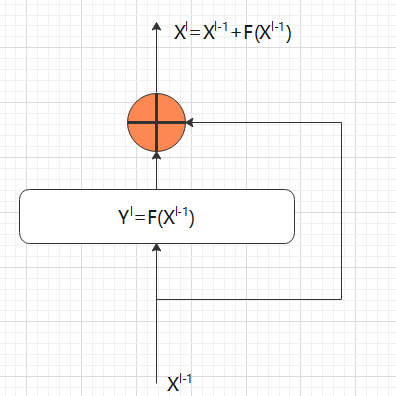
\includegraphics[width=3.5in]{figures/resnet.png}
\caption{残差网络}
\label{fig:resnet}
\end{center}
\end{figure}

\subsection{损失构建方式}
损失函数是现代神经网络的学习目标,通常用来描述模型训练过程中预测值和真实值的差别,假定训练集有$n$个样本$\{(X_i;y_i)|i=1,2,\cdots,n\}$,其中$X_i$表示模型的特征,$y_i$表示模型的标签;模型的预测为$\mathcal{F}(X_i)$。
\subsubsection{分类损失}
对于分类任务,假定模型总共有$n$个类别。模型的标签$y_i$通常是集合$\{1,2,\cdots,n\}$中的一个值的one-hot编码,模型的预测为$\mathcal{F}(X_i)=[p_{i,1},p_{i,2},\cdots,p_{i,n}]$,其中$p_{i,j}$表示模型认为特征$X_i$属于第$j$类的概率,并且满足如下约束:
$$
\sum_{j=1}^{n}p_{i,j}=1
$$
对于分类任务,其损失通常可以使用如下方式计算:
$$
\mathbb{L}=\sum_{i=1}^{n}{y_i*(-log(\mathcal{F}(X_i)^T))}/n
$$
上述计算分类损失的方法,被称为交叉熵损失。
\subsubsection{回归损失}
对于回归任务,模型的标签$y_i$通常是一个实数,模型的预测值$\mathcal{F}(X_i)$也是一个实数。一般来说,模型的预测值和模型的标签值的差越小,表示模型预测越准确;反之表示模型预测越不准确。对于这种类型的问题,构建损失的时候,通常会使用一种被称为均方误差的方式来计算。
$$
\mathbb{L}=\sum_{i=1}^{n}{\sqrt{|y_i-\mathcal{F}(X_i)|^2}}/n
$$
\subsubsection{排序损失}
在自然语言处理领域,涉及到排序的算法,考虑的损失是语意的相似性。通常会给定两个句子$q$和$d$,希望确定这两个句子的语意相关程度$SCORE(q,d)$。最常用的方法是point-wise和pair-wise。point-wise 的方法就是通过负采样,将排序问题构建成一个二分类问题:0表示$q$和$d$不相关,1表示$q$和$d$相关。通常基于point-wise方法的排序问题只有正样本,没有负样本,为了构建分类问题,需要针对每个正样本进行若干负采样,从而构建出二分类的训练集合。模型把两个句子的相关得分定义为将两个文本拼接起来的文本分类为相关的概率作为他们的相关性得分,并依照这个顺序进行排序。

pair-wise 方法最经典的损失构造方法是RankNet中提出的构建损失的方法。这种方法的学习目标是使得逆序对出现的概率尽可能小。通常基于pair-wise方法已知$q$对应的所有文本组成的集合$D=\{d_1,d_2,\cdots,d_m\}$的顺序。假定$s_i=f(q,d_i)$表示$q$和$d_i$的某种相关性得分,$s_j=f(q,d_j)$表示$q$和$d_j$的某种相关性得分。我们记$d_i$比$d_j$和$q$相关性更高为$d_i\triangleright d_j$,那么从模型的视角看来,
$$
p(d_i\triangleright d_j)=\frac{1}{1+e^{-\alpha(d_i-d_j)}}
$$
根据训练样本,我们定义一个指示函数
$$
S_{i,j}=
    \begin{cases}
        1   & if d_i \triangleright d_j\\
        -1  & if d_i \triangleleft d_j\\
        0   & other
    \end{cases}  
$$
那么对于$q$的一个召回句子对,其逆序的损失为
$$
C_{i,j}=-\frac{1}{2}(1+S_{i,j})log(p(d_i\triangleright d_j))-
(1-\frac{1}{2}(1+S_{i,j}))log(p(d_i\triangleright d_j))
$$
有了逆序损失我们就可以构建整体损失了。

\subsubsection{Focal Loss}
在深度学习领域,训练集中通常有些类别的样本数量比较多有些类别的样本数量比较少。对于样本的数量不平衡性,从直觉来讲可以通过加权的方法来处理,也就是对数量较多的样本类的损失进行降权,对于数量较少的样本类的损失进行加权。我们假定第$t$类的第$i$个样本的交叉熵损失为$CE_t(i)$,那么我们可以将样本的损失定义为$\alpha_{t}CE_t(i)$,其中$\alpha_{t}$是经验权重超参数。

在训练集中总是有些样本是容易处理的,其他样本是比较难于处理的。一方面,容易处理的样本数量要远远多于较难处理的样本;另一方面,较难处理的样本通常更有区分度。上述通过加权的方法并没有利用样本难易不同这条信息。Focal Loss就是尝试对容易的样本进行降权来实现的。假定模型将一个属于$t$类的样本$i$分为$t$类的概率为$p_t(i)$,那么这个样本的Focal Loss就可以通过下面的式子来定义:
$$
FL(i)=(1-p_t(i))^{\gamma}CE_t(i)
$$
其中$\gamma>0$是超参数,被称为调制系数。一个样本如果被错分的时候,其$p_t(i)$较小,即这个样本的难度对于模型较难(尚未被正确分类),因此这个样本的损失倾向于不被模型降权;相反如果一个样本本正确分类的时候,其$p_t(i)$较大,即这个样本的难度对于模型来说较容易(已经被正确分类了),因此这个样本的损失倾向于被模型降权。总体来说,Focal loss就是一种能够衡量样本难易度对于分类的贡献度的损失函数。一般样本的数量不平衡性和样本的难易不平衡性是伴生的现象,为了应对这个问题,通常会将上述两种策略融合起来:
$$
FL(i)=\alpha_{t}(1-p_t(i))^{\gamma}CE_t(i)
$$
\section{优化器介绍}
\subsection{标准优化器}
在神经网络优化的时候,通常需要使用梯度下降法。对于标准优化器,根据样本的规模不同可以分为三类:
全样本梯度下降、批量样本梯度下降和随机梯度下降。其中全局梯度下降法会把所有样本的损失的均值作为优化器求梯度的目标函数,假定我们有训练样本集$S={s_i|i=1,2,\cdots,|S|}$,样本$s_i$的损失为$\mathcal{J}(s_i)$。那么对于全局梯度下降法,其参数更新公式如下:
$$
\theta_t = \theta_t - \eta_t \Delta \sum_{s\in S}\mathcal{J}(s)
$$
对于批量随机梯度下降法,首先将训练样本集随机分成若干大小相等的子集$S=S_1\cup S_2 \cup \cdots \cup S_k$。然后按照如下算法来更新梯度:
\begin{algorithm}[h]
    \setstretch{1.3}
    \begin{algorithmic}[1]
    \label{algline:end} 
    \FOR{$\widetilde{S} \in [S_1,S_2, \cdots ,S_k]$} 
       \STATE $\theta_t = \theta_t - \eta_t \Delta \sum_{s\in \widetilde{S}}\mathcal{J}(s)$
       \STATE $t = t + 1$
    \ENDFOR 
    \end{algorithmic}
    \caption{bath-gd($S_1,S_2,\cdots,S_k$)}
    \label{alg:alg1}
\end{algorithm}

如果批量梯度下降法中要求每个子集的元素个数为1,那么批量随机梯度下降算法就退化成是随机梯度下降法。一般来说标准梯度下降算法的的学习率是保持不变的,如果这并不是最优的做法,于是人们提出了若干自适应学习率和标注梯度下降法相结合的优化算法。
\subsection{自适应学习率优化器}
自适应学习率和优化器的结合一直是优化器研究的一个热点,下面我们介绍几个有代表性意义的自适应学习率优化器。
\subsubsection{Adagrad}
Adagrad 是一种基于参数历史更新情况的进行学习率调整的优化器,每个要更新的参数的都维护着表示这一个参数历史更新幅度的量$r_{i,t}$,对于第$t$步迭代假定参数$\theta_i$的梯度是$g_{i,t}$,那么参数更新按照如下步骤执行
$$
\begin{aligned}
r_{i,t} &= r_{i,t} + g_{i,t}^2 \\
\theta_i &= \theta_i-\frac{\eta}{\epsilon + \sqrt{r_{i,t}}}g_{i,t}
\end{aligned}
$$
其中$\eta$是全局学习率,$\epsilon$是平滑参数防止出现分母为零。Adagrad最显著的特征是,不同参数的学习率不同,但是都在随着迭代的进行逐渐变小。显然当一个参数的前期更新幅度过大,那么这个参数到了后期,其更新幅度衰减就会比较厉害;反之如果一个参数的前期更新幅度较小,那么这个参数到了后期,其更新衰减就没有那么厉害。这正是这个学习器自适应调整学习率的核心思想。
\subsubsection{RMSProp}
RMSProp 是针对Adagrad的改进,改进的出发点是对$r_i$的更新引入遗忘因子平滑,使得Adagrad 能够平衡历史和眼前。具体来说第$t$次迭代中,$r_{i,t}$的更新如下
$$
\begin{aligned}
r_{i,t}&=(1-\alpha)r_{i,t-1}+\alpha g_{i,t}^2\\
\theta_i &= \theta_i-\frac{\eta}{\epsilon + \sqrt{r_{i,t}}}g_{i,t}
\end{aligned}
$$
其中$\eta$是全局学习率,$\epsilon$是平滑参数防止出现分母为零,$\alpha$是遗忘因子,通常取值$0.9$。
我将上述公式展开:
$$
\begin{aligned}
r_{i,t}&=\alpha r_{i,t-1}+(1-\alpha) g_{i,t}^2\\
       &=\alpha^2r_{i,t-2}+\alpha g_{i,t-1}^2+(1-\alpha) g_{i,t}^2 \\
       &=\cdots=\\
       &=\alpha^t g_{i,0} +  \alpha^{t-1} g_{i,1} + \cdots + \alpha g_{i,t-1}^2+(1-\alpha) g_{i,t}^2
\end{aligned}
$$
我们看到随着时间推移,历史的梯度更新幅度的贡献逐渐被遗忘,越靠近当前时刻,梯度的的更新对当前学习率的影响越大。这避免了Adagrad一刀切的问题。

\subsection{基于动量的优化器}
在优化器中引入动量就是为了防止优化过程过度震荡问题,使模型的优化方向能够避免反复震荡。可以理解为给优化器引入一个惯性,使优化器能够具有连贯的优化方向。和基于自适应学习率的优化器不同,基于动量的优化器为每个参数维持着一个速度$v_{i,t}$。对于第$t$步迭代假定参数$\theta_i$的梯度是$g_{i,t}$,那么参数更新按照如下步骤执行
$$
\begin{aligned}
m_{i,t}&=\alpha m_{i,t-1} + \beta g_{i,t} \\
\theta_{i,t} &= \theta_{i,t-1} - \eta m_{i,t}
\end{aligned}
$$
相当于当前的梯度更新,需要参考前一时刻梯度惯性的影响,保证优化有一定的连贯性。
\subsection{Adam}
Adam 是一种基于融合了动量和自适应学习率的一种算法,目前是神经网络优化中表现最为出色的一款优化器。我们来介绍着款优化器的细节,首先定义动量和速度,
$$
\begin{aligned}
m_{i,t}&=\beta_1 m_{i,t-1} +(1-\beta_1)g_{i,t} \\
v_{i,t}&=\beta_2 v_{i,t-1} +(1-\beta_2)g_{i,t}^2
\end{aligned}
$$
这里$\beta_1$和$\beta_2$分别表示惯性和速度的遗忘因子,通常$\beta_1$取$0.9$,而$\beta_2$取$0.999$。随后对动量和速度进行遗忘因子的归一化修正,
$$
\begin{aligned}
m_{i,t}&=\frac{m_{i,t}}{1-\beta_1^t} \\
v_{i,t}&=\frac{v_{i,t}}{1-\beta_2^t}
\end{aligned}
$$
最后参数的更新算法按照下面的公式执行,
$$
\theta_{i,t}  =\theta_{i,t-1} -\eta \frac{1}{\sqrt{v_{i,t}}+\epsilon  } m_{i,t} 
$$
\section{防止过拟合相关技术}
所谓过拟合是指随着训练步数的增加或者模型的复杂度的增加,模型的训练损失越来越小,在训练集上的准确度越来越高,但是在测试集上,模型的表现越来越差的现象。比较通俗解释是模型的过拟合是指模型在逐渐拟合训练集的细节,导致其对宏观规律的把握能力下降。解决过拟合现象在数据侧可以通过增加训练集的方法来缓解,在模型侧人们也累积了不少技术手段。主要包括dropout、早停止以及正则化和WeightDecay等手段。
\subsection{dropout 技术}
在训练DNN网络的过程中,对于其中的一层神经元,以一定的概率$p$被随机值置零。这样,在该轮的前馈和反馈中这个值为零的神经元就不会贡献任何信息。在自然语言处理中,dropout 通常有两种用法,一种是在句子Embedding之后执行dropout;另一种是在网络的隐藏层进行dropout。这两种dropout 作用的位置不同,起作用的原理也不同。前者相当于在做数据增强,相当于为给定的句子增加一个随机的噪声,希望模型能够学习到抗噪能力。后者的一种理解是相当于一种网络的集成,由于每次网络的不同单元被置零,相当于网络的结构的变化,因此我们可以理解为模型在训练过程中学到了很多种不同的网络结果,然后将其结果集成起来。
对于全连接层,由于其拟合能力非常强,因此通常会加一些拟合dropout来缓解其中的过拟合现象。
\subsection{早停止技术}
我们知道随着训练步数的增加,模型通常会越来越关注训练集的高频噪声,因此会出现过拟合现象。早停止技术的主要思想是在观测到可能出现过拟合现象的时候,停止训练,从而避免过拟合现象的发生。早停止技术首先将模型分为三个子集——训练集、验证集和测试集。早停止技术在训练过程中,每隔若干步就在验证集上计算一下模型的错误率,当验证集的错误率满足一定条件的时候,我们就提早结束训练过程。一般我们称评估的间隔为评估周期。那么什么时候提早结束训练过程呢?通常有两种做法,我们下面详细介绍这些方法。为了方便我们对于训练到第$t$步,训练集、验证集和测试集的错误率为$E_{tr}(t)$、$E_{va}(t)$和$E_{te}(t)$。
\subsubsection{泛化错误法}
假设$E_{opt}(t)$是模型在训练迭代到第$t$步时,取得最小验证集误差为
$$
E_{opt}(t) = \min_{t'<t}(E_{va}(t'))
$$
这个值通常被称为泛化错误,如果在连续$s$个评估周期上,泛化错误没有降低,就停止训练过程。
\subsubsection{泛化损失法}
我们定义第$t$步的泛化损失为
$$
GL(t)=(\frac{E_{va}(t)}{E_{opt}(t)}-1)
$$
较高的泛化损失表示当前时刻模型的错误率在升高,因此它直接表明了过拟合现象是否发生。当泛化损失高于某个阈值的时候,通常是早停止的时机。


\subsection{正则化和权重衰减}

在人工神经网络发展的历程中,人们发现模型参数的均值和方差较小的时候模型的泛化能力较强,反之模型的泛化能力较弱。因此人们通常会在模型的损失之外增加一个描述模型参数大小的损失。假定存在一个模型,其参数为$\Theta={\theta_i | i=1,2,\cdots,n}$,其模型损失为$\mathbb{J}_m(\Theta)$,那么人们通常会增加一个正则化损失到模型损失上,作为模型的优化目标:
$$
\mathbb{J}(\Theta)=\mathbb{J}_m(\Theta) + \lambda |\Theta|^2
$$
我们对上述的目标关于模型参数求导数,我们得到
$$
\frac{\partial{\mathbb{J}(\Theta)}}{\partial{\Theta}} = \frac{\partial{\mathbb{J}_m(\Theta)}}{\partial{\Theta}} + 2\lambda |\Theta|
$$
那么在梯度下降算法更新参数的时候,我们得到
$$
\Theta = \Theta - \eta( \frac{\partial{\mathbb{J}_m(\Theta)}}{\partial{\Theta}} + 2\lambda |\Theta|)
$$
这显示每次迭代,模型参数都会有一个额外的整数衰减,这种技术就叫L2正则或者权重衰减。需要注意的是Adam优化器会减弱L2正则或者权重衰减的有效性,因此需要使用Adam的一个改进版本——Adamw。现在主流的机器学习框架都有Adamw的开源实现。

\chapter{分词和词向量}

\section{词表最长匹配法}
在深度学习兴起之前人们面对分词任务的时候,最常用的分词方法包括词表最长匹配法和概率法。其中词表最长匹配法是一种启发式的分词法,具体来讲分为前向匹配法、后向匹配法和双向匹配法。词表最大匹配法的问题输入包括词表$V=\{V_1,V_2,\dots,V_N\}$、最大允许的词汇长度$l$和一个完整的句子$S=s_1,s_2,\cdots,s_M$。
\subsection{前向匹配}
前向匹配算法,首先从左到右取长度为$l$的句子段$s_{1+i},s_{2+i},\cdots,s_{l+i}$, 然后判断执行算法1描述的词表匹配逻辑,输出一个新单词$\{C_i\}$并更新句子段的起始位置$i=i + len(C_i)$,直到句子段的起始位置变成句子的结尾,输出分词结果$C=C_1,C_2, \cdots C_K$。当句子段的起始位置$i$接近句末$M$时,句子段可能取不出长为$l$的句子段,此时的句子段取$s_{1+i},s_{2+i},\cdots,s_{M}$作为一个新单词。
\begin{algorithm}[h]
    \setstretch{1.3}
    \textbf{输入:} 句子段$s_{1+i},s_{2+i},\cdots,s_{l+i}$和词表$V=\{v_1,v_2,\dots,v_N\}$\\
    \textbf{输出:}新单词$\{C_i\}$和 句子段的起始位置$i$
    \begin{algorithmic}[1]
        %\label{algline:for} \\
    \FOR{$j := l,l-1,...,1$} \label{algline:end} 
        \IF {$s_{i+1},s_{i+2}\cdots,s_{i+j} \in V$ OR $j = 1$}
         \STATE $C_i:=s_{i+1},s_{i+2}\cdots,s_{i+j}$
         \STATE break \label{algline:break}
        \ENDIF  
    \ENDFOR \label{algline:endfor}
    \STATE \textbf{return} $C_i$ \label{algline:return}
    \end{algorithmic}
    \caption{forward-match($s_{1+i},s_{2+i},\cdots,s_{l+i}$; $V=\{v_1,v_2,\dots,v_N\}$)}
    \label{alg:alg1}
\end{algorithm}
\subsection{后向匹配和双向匹配算法}
后向匹配算法和前向匹配算法的不同点只是匹配的方向不同,前向匹配算法是从左往右匹配,而后向匹配算法是从右往左匹配。具体执行流程这里就不赘述了。一般来说,后向匹配算法效果要优于前向匹配算法。
双向匹配算法是首先对输入的句子执行一次前向匹配和后向匹配,之后通过一些规则来判断前向匹配分词效果好还是后向分词效果好。常见的规则包括分词结果的总词数,单字词数量等。

\section{概率法}
概率分词法中最有影响力的算法主要有两种:基于隐马尔可夫过程(\gls{HMM})的分词法和基于条件随机场(\gls{CRF})的分词法。这两种分词法都属于传统机器学习的范畴,需要比较扎实的数学特别是概率论方面的知识,我们在这里假定读者具备大学概率论方面的基础知识。
\subsection{基于隐马尔可夫过程的分词法}
隐马尔可夫过程是一个比较晦涩难懂的数学概念,理解这个数学概念的关键有两个要素:概率隐变量和马尔科夫性质。首先举个可以用隐马尔科夫过程描述的自然现象,假想有一个人,他日常的活动主要包括打篮球、读书和游泳,在不同的天气条件下,他打篮球和读书的可能性不同,具体如\ref{tab:prob1}表所示。
\begin{table} [h]
    \caption{天气和活动}
	\label{tab:prob1}
	\centering
	\scalebox{0.9}{

\begin{tabular}{l|l|l|l}  % 10cm 減去前兩個欄位寬度後,剩下的通通給  
\hline    
\hline    
&打篮球&读书&游泳\\
\hline                      % 第三欄位使用,文字超出的部份會自動折行  
阴&0.3&0.6&0.1 \\  
\hline  
晴&0.5&0.4&0.1 \\ 
\hline  
雨&0.0&0.9&0.1 \\ 
\hline
雪&0.1&0.7&0.2 \\
\hline
\end{tabular}  }
\end{table}  
而当地的天气变化经过长期的气候分析发现,前一天的天气和当天的天气,符合下面的转移规律,而且通常当天的天气和前天以及更早的天气毫无关联,具体来说当天的天气转移情况如图\ref{tab:prob2}所示。
\begin{figure}[htbp]
\begin{center}
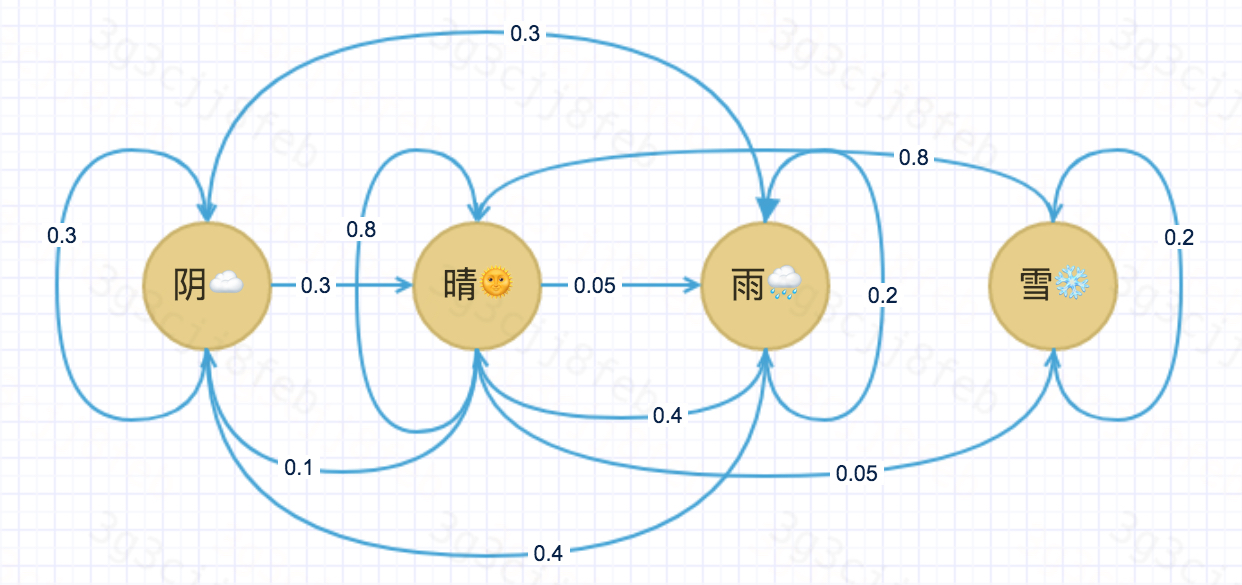
\includegraphics[width=5.5in]{figures/hmm2.png}
\caption{天气转移概率图}
\label{tab:prob2}
\end{center}
\end{figure}


如果我们知道这个人的若干天的活动序列,例如“读书->打篮球->读书->...->打篮球”,天气变化规律和这个人的活动和天气的关系,那么我们能不能估计出这个人所在的城市这些天对应最可能的天气序列呢?事实上,这就是隐马尔可夫过程的预测问题,这个课题已经被很好的解决了。另外,如果我们知道一些这个人的很多天的活动序列和对应的天气序列,那么我们怎么估计这个系统中天气变化的转换规律,怎么估计不同的天气下这个人的活动分布情况呢?事实上这个问题被称为隐马尔可夫过程的有监督学习问题。其实如果仅仅知道这个人的活动序列也是有可能估计出这个系统中天气变化的转换规律和不同的天气下这个人的活动分布情况的。这个问题被称为隐马尔可夫过程的无监督学习问题。有监督学习问题和无监督学习问题统称马尔科夫的学习问题。下面我们铺垫一些数学知识,然后仔细介绍如何将分词问题是如何建模成隐马尔可夫的学习问题和预测问题的。


\subsubsection{隐马尔可夫过程}
一个隐马尔可夫过程通常由一个五元祖构成$\{O,S,\Pi,T,E\}$,分别表示观察序列$O=[o_1,o_2,\cdots,o_{|O|}]$,其中观察序列的取值范围是一个离散的集合$W=\{w_1, w_2,\cdots,w_{|W|}\}$;隐藏序列$H=[h_1,h_2, \cdots h_{|H|}]$, 其中隐藏序列的取值范围也是一个离散的集合$V=\{v_1,v_2,\cdots,v_{|V|}\}$; 隐藏状态转移矩阵$T=\{t_{i,j}|t_{i,j}=P(v_j|v_i); i,j \in [1,2,\cdots,|V|]\}$; 隐状态初始分布矩阵$\Pi=[\pi_1,\pi_2,\cdots \pi_{|V|}]$;和隐藏状态到观察状态的发射概率$E=[e_{i,j} | e_{i,j}=P(o_j|h_i);i\in[1,2,\cdots,|V|],j\in[1,2,\cdots,|W|]]$组成。在上面的例子中活动序列对应这里的观察序列,活动序列的取值集合为{打篮球,读书,游泳};活动序列对应的天气序列是隐藏序列,隐藏序列的取值集合为{阴,晴,雨,雪};另外这个人的在不同天气下的活动分布对应这里的发射概率;最后,这个系统的天气自然发生率是初始概率。我们上面的例子中提到的地方的天气很怪,当天的天气仅仅和昨天的天气有关系,和前天的天气没有丝毫关联。其实我们可以把天气的阴晴雨雪发生,当做上帝在玩一个概率游戏,这个游戏就是根据前一天的天气,选择一个四面的筛子,这个筛子不同面的概率是不同。针对上面的例子我们,前一天不同天气对应的筛子如表\ref{tab:prob3}所示。
\begin{table} [h]
    \caption{天气筛子游戏}
	\label{tab:prob3}
	\centering
	\scalebox{0.9}{
\begin{tabular}{l|l}  % 10cm 減去前兩個欄位寬度後,剩下的通通給  
\hline                      % 第三欄位使用,文字超出的部份會自動折行  
前一天的天气& 生成当天天气的筛子规格\\
\hline
阴 & 阴:0.3,晴:0.3,雨:0.4,雪:0.0\\
\hline  
晴 & 阴:0.1,晴:0.8,雨:0.05,雪:0.05\\
\hline  
雨& 阴:0.3,晴:0.4,雨:0.2,雪:0.1\\
\hline  
雪& 阴:0.0,晴:0.8,雨:0.0,雪:0.2\\
\hline
\end{tabular}  
}
\end{table}  
我们可以看出这个筛子游戏中当天的天气仅仅受前一天的天气影响,这种性质被称为马尔科夫性。用数学的语言描述就是
$$
p(h_t|h_1,h_2, \cdots h_{t-1}) = p(h_t|h_{t-1})
$$

隐马尔科夫过程主要研究三个课题:概率计算问题、学习问题和预测问题。其中概率计算问题是指已知模型的参数,求一个给定观察序列的出现概率;学习问题是指已知观察序列或者观察序列和隐藏序列都知道,求解模型参数;预测问题是指已知模型参数求给定观察序列,求最有可能的隐藏序列。这三个问题是隐马尔可夫过程的重要课题都已经被很好的解决了。
针对概率计算问题,人们通常使用前向概率计算法和后向概率及算法来解决;针对学习问题,如果是非监督学习最为常用的方法是EM算法,如果是监督学习最常用的方法是频率估计法;针对预测问题,可以通过维特比算法来解决,下面我们具体介绍一下这三个课题和相应的解法。

$-$  \textbf{计算问题}
\begin{definition}
概率计算问题的输入是五元组中的$O$和模型参数$\{V,T,Pi\}$,求解已知模型参数的前提下,计算一个给定观察序列的出现概率:$P(O;V,T,Pi)$。
\end{definition}


这个问题的困难之处是所有的隐藏序列都可以以一定的概率产生观察序列。假定隐藏序列和其出现的概率分别为$\hat{H}_i=[\hat{h}_{i,1},\hat{h}_{i,2},\cdots,\hat{h}_{i,|H|}]$ 和$\hat{P}_i$,那么
$$
P(O;V,T,P_i)=\sum_{i}{\hat{P}_i\prod_{j\in\{1,2,\cdots,|H|\}}{P(o_{i,j}|\hat{h}_j)}}
$$
隐藏序列的生成分两个步骤:第一个步骤由初始概率分布产生第一个隐藏状态,第二个步骤根据概率转移矩阵和前一个隐藏状态逐步生成一个隐藏状态。可以看出这里有两个概率发生器:
\begin{itemize}
 \item 初始状态概率发生器,这个发生器不需要输入就可以根据初始状态分布矩阵$\Pi=[\pi_1,\pi_2,\cdots \pi_{|V|}]$,就可以随机产生第一个隐藏状态$h_i$并给出其出现的概率$P(h_i)$;
 \item 递归状态发生器,这个发生器需要前一个时刻的隐藏状态$h_{i-1}$作为输入,并根据 隐藏状态转移矩阵$T=\{t_{i,j}|t_{i,j}=P(v_j|v_i); i,j \in [1,2,\cdots,|V|]\}$生成下一个时刻的隐藏状态$h_{i}$,并给出发生概率:
 $
 P(h_i|h_{i-1}) = t_{i,i-1}
 $
\end{itemize}
我们知道长度为$k$的隐藏序列,是由长度为$k-1$的隐藏序列,通过第二个序列发生器生成第$k$个隐藏状态构造出来的。我们知道长度为$k-1$的隐藏序列的末尾元素取值范围是$V=\{v_1,v_2,\cdots,v_{|V|}\}$,而长度为$k$的隐藏序列的最后一个元素仅和$k-1$时刻有关(马尔可夫性质),因此可以根据长度为$k-1$的隐藏序列的信息和前$k-1$个观察序列出现的概率,和转移概率计算出长度为$k$的隐藏序列到前$k$个观察序列出现的概率。假定以$v_i$结尾长度为$k-1$的隐藏序列到前$k-1$个观察序列出现的概率为$P(v_i*,k-1)$, 那么以$v_j$结尾长度为$k$的隐藏序列到前$k$个观察序列出现的概率$P(v_j*,k)$就可以根据下面的公式计算出来:
$$
P(v_j*,k)=\sum_{i\in{1,2,\cdots,|V|}}{P(v_i*,k-1)t_{i,j}P(\hat{o}_i|h_j)}
$$
这样问题就被可以被动态规划算法来解决,因为到目前为止我们已经定义清楚了最优子结构和重叠子问题,最优子结构和重叠子问题的概念如果大家不清楚,可以参考《算法导论》。
最后,由于$t$时刻的观察序列可能是由任何一个同时刻的状态产出的,所以根据概率加法原理:
$$P(O;V,T,Pi)=\sum_{i\in{1,2,\cdots,|V|}}P(v_j*,|H|)$$


$-$  \textbf{预测问题}
\begin{definition}
预测问题的输入是五元组中的$O$和模型参数$\{V,T,\Pi\}$,求解已知模型参数的前提下,计算一个给定观察序列的条件下,最有可能的隐藏序列$H$。
\end{definition}
这个问题需要逐步生成每一个时刻的隐藏序列,类似seq2seq中的解码问题,所以也被称为解码问题。我们在后续的章节中会详细介绍seq2seq的解码问题,这个问题的解法中最著名的是维特比算法。
维特比算法是大名鼎鼎的通信专家高通公司创始人安德鲁维特比发明的。和计算问题类似,维特比算法是一种动态规划算法,动态规划问题主要是找到最优子结构和重叠子问题。事实上我们通过解计算问题,可以构建一张表,这张表如图\ref{fig:hmm3}所示.
\begin{figure}[htbp]
\begin{center}
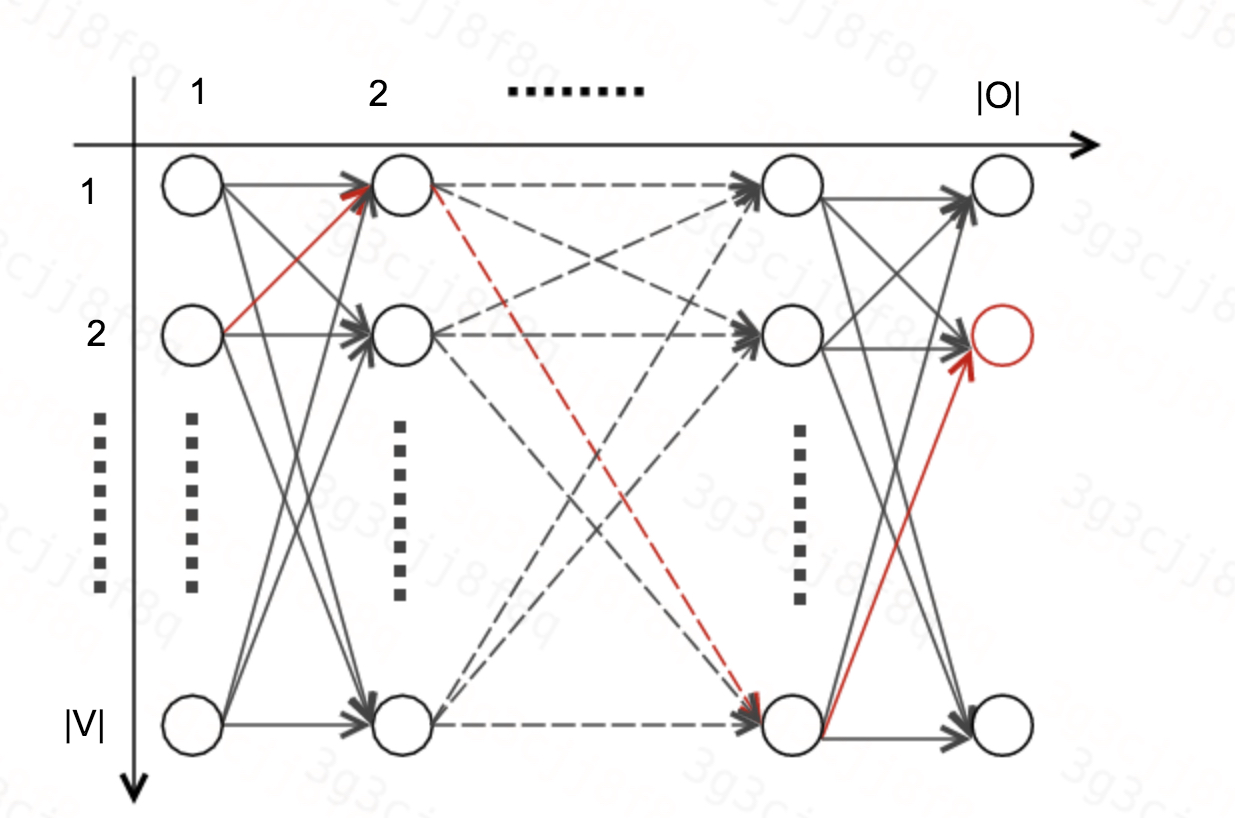
\includegraphics[width=5.5in]{figures/hmm3.png}
\caption{维特比解码算法示意图} \label{fig:hmm3}
\label{default}
\end{center}
\end{figure}
第$k$行第$i$列表示$P(v_i*,k)$。我们从最后一列,我们可以得知$|O|$时刻以哪个隐藏状态结尾,最有可能生成观察序列$[o1,o_2,\cdots,\o_{|O|}]$,所以最后一个时刻的隐藏状态可以据此解出。然后我们后退一个时刻,后退的时候我们知道退到哪个隐藏状态,可以保证最后时刻输出最大概率,从可解除第$|O|-1$时刻的符号。依次类推,可以完整解除最优可能的隐藏序列。


$-$ \textbf{学习问题}
\begin{definition}
有监督学习问题,在隐马尔可夫过程中,有监督学习问题是指给定观察序列和隐藏序列对的条件下,求模型参数的问题。
\end{definition}
\begin{definition}
无监督学习问题,在隐马尔可夫过程中,无监督学习问题是指仅给定观察序列的条件下,求模型参数的问题。
\end{definition}

其中有监督的方法比较容易理解,通常是使用频率来近似概率即可。无监督的方法比较晦涩,涉及到传统机器学习中的一个重要方法——EM算法。这个EM算法比较晦涩难懂,如果展开的话,可能需要较大的篇幅,我们把这部分内容放到了附件中。对于有监督学习我们需要估计三个参数,其估计方法如下:
\begin{enumerate}
\item 初始概率矩阵$\Pi$的估计

初始概率矩阵的估计最为简单,只要统计一下所有隐藏序列中隐藏状态的发生次数$F_i$做一下归一化就行了:
$$
\pi_{i}=\frac{F_{i}}{\sum_{k}{F_{k}}}
$$
\item 转移概率矩阵$T$的估计

统计所以隐藏序列中,隐藏状态从$v_i$转换到$v_j$发生的次数$F_{i,j}$, 那么隐状态$v_i$到$v_j$的转移概率$
t_{i,j}$可以用下面的式子估计:
$$
t_{i,j}=\frac{F_{i,j}}{\sum_{k}{F_{i,k}}}
$$
\item 发射概率矩阵$E$的估计

统计每个平行序列对对应时刻的隐藏状态$v_i$和对应的观察状态$w_j$ 发生的次数$F_{i,j}$,那么,从隐藏状态$v_i$发射到观察状态$w_j$的发生概率$e_{i,j}$可以用下面的式子估计:
$$
e_{i,j}=\frac{F_{i,j}}{\sum_{k}{F_{i,k}}}
$$

\end{enumerate}


最后我们给出一个\gls{HMM}常见问题解的python实现:
\begin{lstlisting}[language={python}]
import numpy as np


class HMM:
	"""
	Order 1 Hidden Markov Model
	Attributes
	----------
	A : numpy.ndarray
			State transition probability matrix
	B: numpy.ndarray
			Output emission probability matrix with shape(N, number of output types)
	pi: numpy.ndarray
			Initial state probablity vector
	Common Variables
	----------------
	obs_seq : list of int
			list of observations (represented as ints corresponding to output
			indexes in B) in order of appearance
	T : int
			number of observations in an observation sequence
	N : int
			number of states
	"""

	def __init__(self, A, B, pi):
		self.A = A
		self.B = B
		self.pi = pi

	def _forward(self, obs_seq):
		N = self.A.shape[0]
		T = len(obs_seq)

		F = np.zeros((N, T))
		F[:, 0] = self.pi * self.B[:, obs_seq[0]]

		for t in range(1, T):
			for n in range(N):
				F[n, t] = np.dot(F[:, t - 1], (self.A[:, n])) * self.B[n, obs_seq[t]]

		return F

	def _backward(self, obs_seq):
		N = self.A.shape[0]
		T = len(obs_seq)

		X = np.zeros((N, T))
		X[:, -1:] = 1

		for t in reversed(range(T - 1)):
			for n in range(N):
				X[n, t] = np.sum(X[:, t + 1] * self.A[n, :] * self.B[:, obs_seq[t + 1]])

		return X

	def observation_prob(self, obs_seq):
		""" P( entire observation sequence | A, B, pi ) """
		return np.sum(self._forward(obs_seq)[:, -1])

	def state_path(self, obs_seq):
		"""
		Returns
		-------
		V[last_state, -1] : float
				Probability of the optimal state path
		path : list(int)
				Optimal state path for the observation sequence
		"""
		V, prev = self.viterbi(obs_seq)

		# Build state path with greatest probability
		last_state = np.argmax(V[:, -1])
		path = list(self.build_viterbi_path(prev, last_state))

		return V[last_state, -1], reversed(path)

	def viterbi(self, obs_seq):
		"""
		Returns
		-------
		V : numpy.ndarray
				V [s][t] = Maximum probability of an observation sequence ending
									 at time 't' with final state 's'
		prev : numpy.ndarray
				Contains a pointer to the previous state at t-1 that maximizes
				V[state][t]
		"""
		N = self.A.shape[0]
		T = len(obs_seq)
		prev = np.zeros((T - 1, N), dtype=int)

		# DP matrix containing max likelihood of state at a given time
		V = np.zeros((N, T))
		V[:, 0] = self.pi * self.B[:, obs_seq[0]]

		for t in range(1, T):
			for n in range(N):
				seq_probs = V[:, t - 1] * self.A[:, n] * self.B[n, obs_seq[t]]
				prev[t - 1, n] = np.argmax(seq_probs)
				V[n, t] = np.max(seq_probs)

		return V, prev

	def build_viterbi_path(self, prev, last_state):
		"""Returns a state path ending in last_state in reverse order."""
		T = len(prev)
		yield (last_state)
		for i in range(T - 1, -1, -1):
			yield (prev[i, last_state])
			last_state = prev[i, last_state]

	def baum_welch_train(self, obs_seq):
		N = self.A.shape[0]
		T = len(obs_seq)

		forw = self._forward(obs_seq)
		back = self._backward(obs_seq)

		# P( entire observation sequence | A, B, pi )
		obs_prob = np.sum(forw[:, -1])
		if obs_prob <= 0:
			raise ValueError("P(O | lambda) = 0. Cannot optimize!")

		xi = np.zeros((T - 1, N, N))
		for t in range(xi.shape[0]):
			xi[t, :, :] = self.A * forw[:, [t]] * self.B[:, obs_seq[t + 1]] * back[:, t + 1] / obs_prob

		gamma = forw * back / obs_prob

		# Gamma sum excluding last column
		gamma_sum_A = np.sum(gamma[:, :-1], axis=1, keepdims=True)
		# Vector of binary values indicating whether a row in gamma_sum is 0.
		# If a gamma_sum row is 0, save old rows on update
		rows_to_keep_A = (gamma_sum_A == 0)
		# Convert all 0s to 1s to avoid division by zero
		gamma_sum_A[gamma_sum_A == 0] = 1.
		next_A = np.sum(xi, axis=0) / gamma_sum_A

		gamma_sum_B = np.sum(gamma, axis=1, keepdims=True)
		rows_to_keep_B = (gamma_sum_B == 0)
		gamma_sum_B[gamma_sum_B == 0] = 1.

		obs_mat = np.zeros((T, self.B.shape[1]))
		obs_mat[range(T), obs_seq] = 1
		next_B = np.dot(gamma, obs_mat) / gamma_sum_B

		# Update model
		self.A = self.A * rows_to_keep_A + next_A
		self.B = self.B * rows_to_keep_B + next_B
		self.pi = gamma[:, 0] / np.sum(gamma[:, 0])
\end{lstlisting}

\subsubsection{隐马尔可夫过程分词}

$-$ \textbf{分词数据的标注方法}

分词任务的训练数据通常是一些列平行序列,每个平行序列包含两个部分:汉字序列$O=[o1,o2,\cdots,o_{|O|}]$;标注序列$H=[h_1,h_2, \cdots h_{|H|}]$。通常训练数据的标注有两种方法:BI和BMES,BI是begin和inner的首字符,分别表示对应位置的汉字是一个词语的开始位置和中间位置;BMES是begin、media、end和single的首字符,分别表示对应位置的汉字是一个词语的开始位置、中间位置、结束位置和单字成词。表\ref{tab:fenci}就是一个例子。

\begin{table} [h]
    \caption{分词示例}
	\label{tab:fenci}
	\centering
	\scalebox{0.9}{
\begin{tabular}{l|l|l|l|l|l|l|l|l|l|l|l|l|l|l|l|l}  % 10cm 減去前兩個欄位寬度後,剩下的通通給  
\hline                      % 第三欄位使用,文字超出的部份會自動折行  
汉字序列&我&是&一&个&热&爱&自&然&语&言&处&理&的&好&学&生 \\  
\hline  
BI&B& B& B& I& B& I& B& I& I& I& I& I& B& B& I& I \\ 
\hline  
BMES&S& S& B& E& B& E& B& M& M& M& M& E& S& B& M& E \\ 
\hline  
\end{tabular}  }
\end{table}  

$-$ \textbf{HMM概率分词模型}

如果我们使用\gls{HMM}作为分词算法,算法分为两个步骤,的第一个步骤是根据训练语料学习模型参数,我们称之为学习过程;第二个步骤是使用维特比算来预测模型,我们称之为解码过程。使用\gls{HMM}模型的时候,汉字序列我们当做观察序列$O=[o1,o2,\cdots,o_{|O|}]$,标注序列我们当做隐藏序列$H=[h_1,h_2, \cdots h_{|H|}]$。另外我们假设模型的标注序列仅和前一个时刻的标注状态有关,也就是说标注序列符合马尔科夫性质。到此为止,我们已经完成了分词问题的数学建模。我们只需要使用有监督的方法,学习出模型的参数,这组参数包含了分词概率系统的数学信息;之后就可以基于这些数学信息使用维特比算法来根据给定的汉字序列求出其最有可能的标注序列了,有了标注序列我们就知道哪些汉字属于同一个词汇。如果使用\gls{HMM}模式,使用著名的jieba分词工具进行汉语分词的时候,就是在调用维特比算法。

需要注意的是如果使用BMES标注法,有一些特殊的情况需要处理,比如M状态不能转为B状态也不能转成S状态;BI标注法没有这个限制。


\section{Subword 技术}
如果把完整汉语词汇都考虑进词表里面,词表的大小可能会多达十万甚至数十万条之多,这对于训练词向量,语言模型和神经网络机器翻译都是巨大的挑战,一方面embedding矩阵和最后的project层参数都会非常大,另一方面由于很多词汇非常生僻,因此得不到很好的训练,从而干扰模型的性能。所以,通行的做法是人们取最为常用的前几千或者几万词汇作为词表,但是这样以来会有数量可观的词汇不在词表中,这些不在词表中的词同样会影响模型的表现,这个问题被称为\gls{OOV}问题。一些计算机学家在研究机器翻译问题的时候,为了缓解\gls{OOV}问题,提出了双字节编码的方法。

该算法最早在1994年2月被Philip Gage 在其文章《A New Algorithm for Data Compression》 中提出来的,这个算法最初的用途是数据压缩。直到2016年,有学者提出使用\gls{BPE}编码技术可以有效缓解机器翻译中的OOV问题,后来的一些研究,特别是著名的\gls{BERT}也延用了\gls{BPE}编码作为自己的分词手段,这种技术才逐渐被人们认识和广泛应用。\gls{BPE}算法的思想非常朴素,其核心就是用一个字符去替换最频繁出现的双字符,然后对替换序列继续之上上述操作,直到连续连个字符出现的频率都小于一个阈值截止。

Subword 工具推荐大家使用SentencePiecem,SentencePiece是一个google开源的自然语言处理工具包。面向神经网络文本生成系统的无监督文本词条化工具。

\section{词向量}

将词语转换成一个数学量一直以来就是广大计算机学家的夙愿,因为向量可以进行加法、减法、点乘和叉乘等诸多运算,如果词汇能够向量化,那么语义计算就变得可能。一个可以设想的应用就是可以通过定义距离来定义词汇之间语义的近似程度,当然现在的神经网络词向量算法已经基本上能够支持这个运算了。文本一直被认为是非结构化的不可计算的数据,词向量化是文本数据向结构化可计算化迈出的关键性步骤。这一步最早的有影响力的研究出自Google,他们提出两种计算词向量的浅层模型:\gls{CBOW} 和 Skip-gram。

在此之前,惯常的做法是使用one-hot编码,所谓one-hot编码就是每个词都表示成一个$1\times N$ 的矩阵,
$$
V = \begin{pmatrix}
v_1,v_2,\cdots,v_N
\end{pmatrix}
$$
这个矩阵中只有一个位置是$1$,其他位置都是$0$, 其中$N$ 通常是词表的大小。显然,这种词向量没有任何语义可言。于是很多研究者会先生成一个可训练矩阵
$$
M=\begin{pmatrix}
m_{1,1}&m_{1,2}&\cdots&m_{1,E} \\
m_{2,1}&m_{2,2}&\cdots&m_{2,E} \\
\vdots &\vdots & \ddots & \vdots \\
m_{N,1}&m_{N,2}&\cdots&m_{N,E} 
\end{pmatrix}
$$
然后通过下面的矩阵运算求出词的可训练表示:
$$
\hat{V} =  
\begin{pmatrix}
v_1,v_2,\cdots,v_N
\end{pmatrix}
\begin{pmatrix}
m_{1,1}&m_{1,2}&\cdots&m_{1,E} \\
m_{2,1}&m_{2,2}&\cdots&m_{2,E} \\
\vdots &\vdots & \ddots & \vdots \\
m_{N,1}&m_{N,2}&\cdots&m_{N,E} 
\end{pmatrix}
$$
上述过程在\gls{NLP}领域一般被称为随机Embedding。
那么怎么去构造损失函数求解最优的Embedding呢?因为在深度学习领域,如果没有损失函数,我们什么也做不了。\gls{CBOW} 和 Skip-gram就是两种设计损失函数的方法。大量的实验表明使用预训练出来的词向量能够在很大程度上改善模型的表现,表
	\label{tab:prob4}是在TextCNN中使用预训练Embedding和随机Embedding在若干个公开数据集合上的对比,我们看到平均有4到5个百分点的提升。
\begin{table} [h]

	\label{tab:prob4}
	\centering
	\scalebox{0.9}{
\begin{tabular}{lccccccc}  % 10cm 減去前兩個欄位寬度後,剩下的通通給 
\toprule
Model &MR& SST-1& SST-2& Subj& TREC& CR& MPQA\\
\hline
\gls{CNN}-rand& 76.1& 45.0& 82.7& 89.6& 91.2& 79.8& 83.4\\
\gls{CNN}-pretrain& 81.5& 48.0& 87.2& 93.4& 93.6& 84.3& 89.5\\
\bottomrule
\end{tabular}
}
\end{table}

\subsection{CBOW}
\gls{CBOW} 的基本思想是在一个自然形成的有意义的句子中,如果我们从中扣掉了其中的若干词汇,是有可能通过上下文将其重建出来的,而这个重建的过程会用到其他位置的词的语义信息。图\ref{fig:cbow1}是\gls{CBOW}的基本网络结构,可以看出是一个浅层的网络。这个网络首先将样本涉及的词转换成one-hot编码$c_i$,然后乘以一个随机初始化的矩阵$W$。根据矩阵乘法运算规则,$c_iW$ 等价于从$W$ 中选出$c_i$元素为1的下标对应的$W$中的那一列。之后所有取出的列求和后形成一个中间结果,然后这个中间结果透过线性投射层去预测窗口中心词。

\begin{figure}[htbp]
\begin{center}
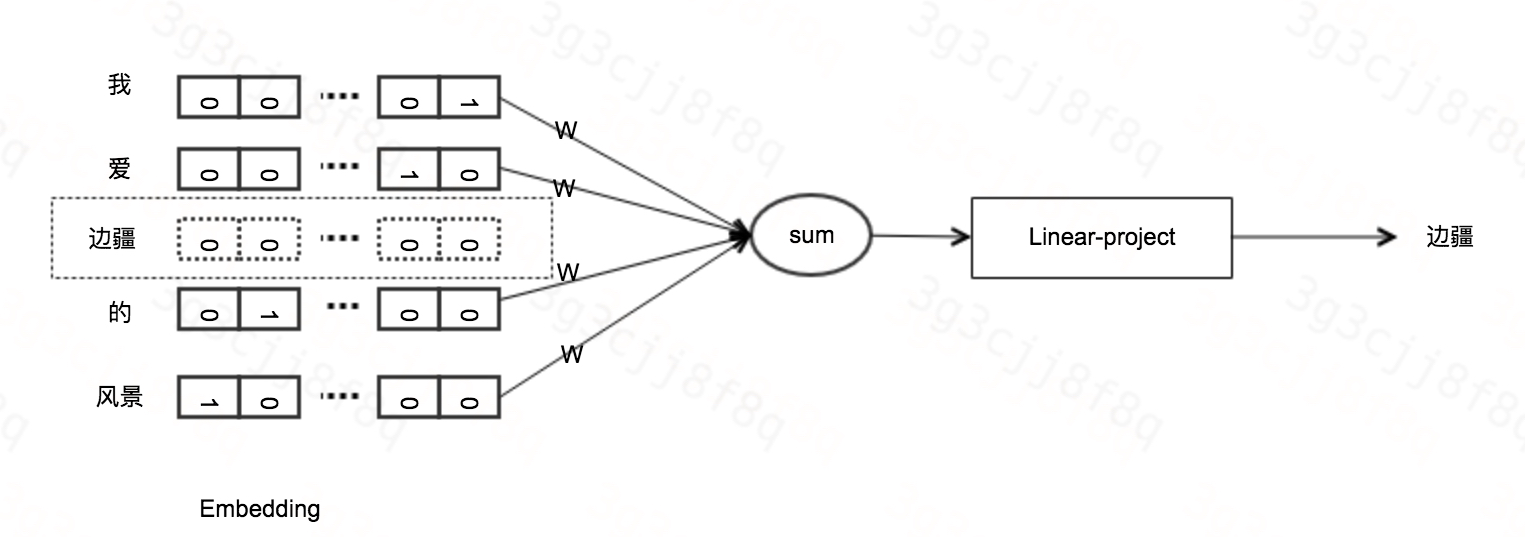
\includegraphics[width=5.5in]{figures/cbow1.png}
\caption{CBOW 网络结构}\label{fig:cbow1}
\label{fig:cbow1}
\end{center}
\end{figure}

这个网络的输入是一个句子,然后在这个句子上定义一个窗口,通常这个窗口的大小是奇数,我们把窗口中心的词作为预测对象,把其他位置的词作为预测中心词的特征。例如输入的句子是"我们 都有 一个 家 名字 叫 中国",可以形成的训练样本为表1.4所示。
\begin{table} [h]

	\label{tab:schedule}
	\centering
	\scalebox{0.9}{
\begin{tabular}{l|l}  % 10cm 減去前兩個欄位寬度後,剩下的通通給  
\hline                      % 第三欄位使用,文字超出的部份會自動折行  
\hline  
特征&正样本\\  
\hline  
我们,一个&都有 \\ 
\hline  
都有,家&一个 \\ 
\hline  
一个,名字&家 \\
\hline  
家,加&名字 \\
\hline  
\end{tabular}  
}
\caption{可用特征构造}  
\end{table}  

如果不加处理,上述分类是一个$N$分类问题,$N$ 是词表的大小,汉字的常用词可能有数万甚至更多,因此上述问题是一个标签超大规模的分类问题,在最后的softmax层计算量比较大。为了降低训练的计算量,常见的做法法是使用采样的方法,简单来说就是通过采样计算期望的思路通过多个二分类来近似计算最后的超大规模softmax,实验证明随机采样20个左右的负样本即可非常接近原始softmax,这种技术的数学原理比较繁琐,这里就不展开了,有兴趣的读者可以自己去阅读相关的论文。事实上,这种做法最早是用来加速语言模型的训练的,不过用在\gls{CBOW}模型里也非常合适,我们可以把\gls{CBOW}看成是一种窗口化的掩码语言模型。关于掩码语言模型我们会在后续的章节详细介绍。超大规模softmax的采样加速算法在tensorflow 框架下,通常使用下面的API来实现:


\begin{lstlisting}[language={python}] 
def sampled_softmax_loss(weights,
                         biases,
                         labels,
                         inputs,
                         num_sampled,
                         num_classes,
                         num_true=1,
                         sampled_values=None,
                         remove_accidental_hits=True,
                         partition_strategy="mod",
                         name="sampled_softmax_loss",
                         seed=None)  
\end{lstlisting}  



需要注意的是,使用这个API的时候需要在生成词到词ID的映射时,频率大的ID小,原因是$sampled\_softmax\_loss$认为词汇在词表中的分布服从zipfan分布,并使用这个分布进行采样,这个采样的在计算的时候需要上述对ID映射的规定。如果不按照约定来生成词表,那么采样可能存在偏差。\gls{CBOW}的完整代码参见:

\begin{lstlisting}[language={python}]
tf_train_dataset = tf.placeholder(tf.int32, shape=(batch_size, 2*half_window_size))
tf_train_labels = tf.placeholder(tf.int32, shape=(batch_size, 1))
tf_valid_dataset = tf.constant(valid_examples, dtype=tf.int32)

embeddings = tf.Variable(tf.random_uniform(shape=(vocabulary_size, embedding_size), minval=-1.0, maxval=1.0))
softmax_weights = tf.Variable(tf.truncated_normal(shape=(vocabulary_size, embedding_size), stddev=1.0 / math.sqrt(embedding_size)))
softmax_biases = tf.constant(np.zeros(shape=(vocabulary_size), dtype=np.float32))

embed = tf.nn.embedding_lookup(embeddings, tf_train_dataset)
inputs = tf.reduce_sum(embed, 1)
loss = tf.reduce_mean(
		tf.nn.sampled_softmax_loss(
								softmax_weights, softmax_biases, inputs, tf_train_labels, num_sampled, vocabulary_size
							)
						)
\end{lstlisting}


\subsection{Skip-gram}
Skip-gram 是另外一种语义建模的方法,这种建模方法同样是基于滑动窗口的,Skip-gram 构造样本的方法与\gls{CBOW}方法正好反过来,前者通过周围的词预测窗口中心词,后者通过窗口中心词预测窗口中的其他词汇,从而取挖掘词向量的合理表示。这种方法直觉上感觉不是非常靠谱,因为单个词汇去预测很多的词汇,这个听起来不是非常靠谱,但是研究结果表明,其效果并不比\gls{CBOW}差甚至更好。我个人的理解是,Skip-gram 构造了一个相对困难的任务,从而逼迫模型利用有限的词向量去表示语义,甚至进行语义联想,所以大规模训练语料中蕴含的语义知识能被合理的内化到词向量的表示中。当然Skip-gram构建特征时候使用的滑动窗口不能太大,一般取3到5个,因为窗口如果太大,边缘的词语和窗口中心词之间的语义关系就会变得非常微弱,从而影响模型的收敛。Skip-gram 的模型结构如下, 窗口中心词首先经过one-hot编码之后$c_i$, 乘以一个随机初始化的矩阵$W$, 根据矩阵乘法运算规则,$c_iW$ 等价于从$W$ 中选出$c_i$元素为1的下标对应的$W$中的那一列。之后这个取出的列矩阵通过不同的线性投射层去预测不同位置的窗口其他词。

\begin{figure}[htbp]
\begin{center}
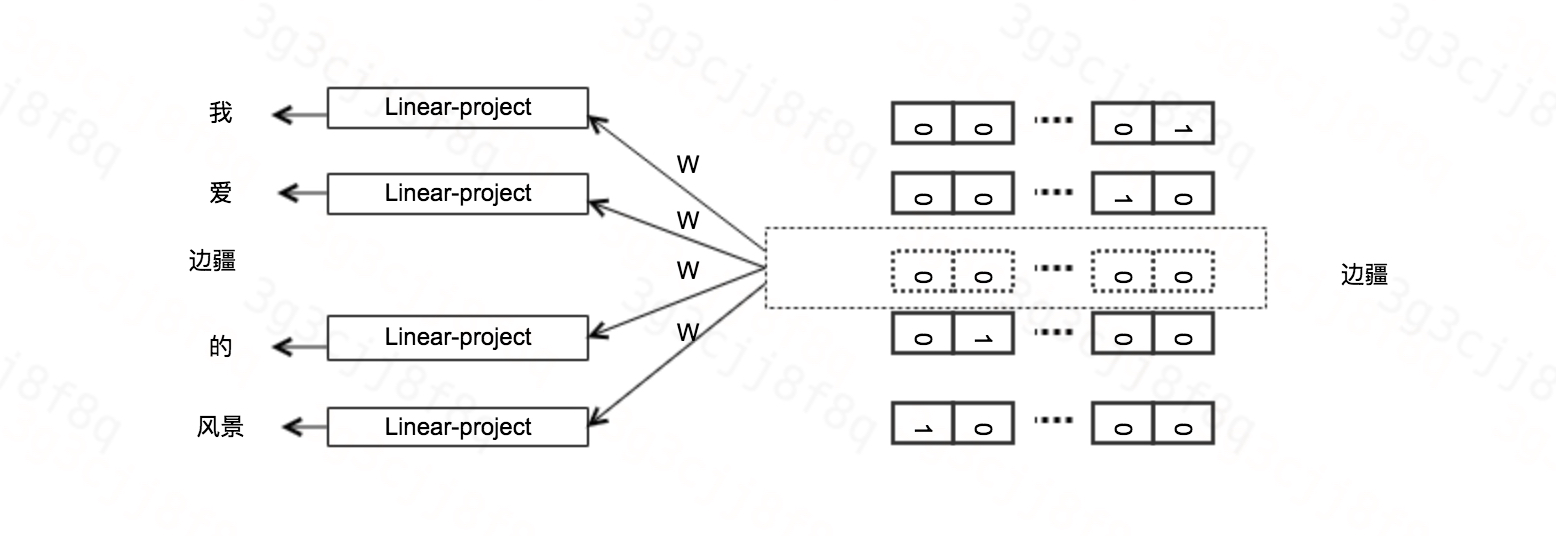
\includegraphics[width=5.8in]{figures/skip-gram1.png}
\caption{Skip-gram 网络结构}
\label{fig:skip-gram1}
\end{center}
\end{figure}
Skip-gram的关键代码如下, 同样我们看到Skip-gram 可以使用采样策略进行训练加速。

\begin{lstlisting}[language={python}]
# Input data.
	train_dataset = tf.placeholder(tf.int32, shape=[batch_size])
	train_labels = tf.placeholder(tf.int32, shape=[batch_size, 1])
	valid_dataset = tf.constant(valid_examples, dtype=tf.int32)

	# Variables.
	embeddings = tf.Variable(
						tf.random_uniform([vocabulary_size, embedding_size], -1.0, 1.0))
	softmax_weights = tf.Variable(
						tf.truncated_normal([vocabulary_size, embedding_size],
											stddev=1.0 / math.sqrt(embedding_size)))
	softmax_biases = tf.Variable(tf.zeros([vocabulary_size]))

	# Model.
	# Look up embeddings for inputs.
	embed = tf.nn.embedding_lookup(embeddings, train_dataset)
	# Compute the softmax loss, using a sample of the negative labels each time.
	loss = tf.reduce_mean(
						tf.nn.sampled_softmax_loss(softmax_weights, softmax_biases, embed,
													train_labels, num_sampled, vocabulary_size))
\end{lstlisting}
\subsection{Glove}
\gls{CBOW}和skip-gram虽然可以很好地进行词汇类比,但是因为这两种方法是基于一个局部的上下文窗口方法的,因此没有有效地利用全局的词汇共现统计信息。为了克服局部上下文窗口的缺陷,在2014年,Jeffrey Pennington等人提出了一种新的\gls{Glove}方法,该方法基于全局词汇共现的统计信息来学习词向量,从而将统计信息与局部上下文窗口方法的优点都结合起来,并发现其效果确实得到了提升。

在介绍\gls{Glove}的原理之前,先来看论文中的一个案例,假设有两个词$w_i$:冰和水蒸气。其关联词取不同的词汇$w_k$,如“固态”,“液态”和“气态”等,根据上面的定义,我们分别计算他们的概率$P(w_{k}|w_{i})$。可以想象,对于“冰”,其出现在“固态”的上下文概率应该比较大,出现在“气态”上下文的概率应该比较小,因此,他们的比值应该是一个比较大的数,;而对于“水蒸气”,出现在“固态”上下文的概率应该比较小,而出现在“气态”上下文的概率应该比较大,因此,两者的比值应该是一个比较小的数。而对于“液态”这个词汇,他们与“冰”和“水蒸气”的相关性应该比较小,因此,他们的比值应该都是接近1。因此,这样来看可以发现,比值$P(w_k | w_i)$在一定程度上可以反映词汇之间的相关性,当相关性比较低时,其值应该在1附近,当相关性比较高时,比值应该偏离1比较远。

但是这个如何跟词向量建立联系呢?我们假定存在一个关于词向量的函数$F(w_i,w_j,w_k)$能够描述上述比值,我们一步步看有没有合适的函数能够构造出来,目前已知:
$$
F(w_i,w_j,w_k)=\frac{p(w_i|w_k)}{p(w_j|w_k)}
$$
既然想反应语义的差异,我们想到的是先对上下文词汇的两个关联词向量做差,所以上述关系通过下面的表示来表达:
$$
F(w_i-w_j,w_k)=\frac{p(w_i|w_k)}{p(w_j|w_k)}
$$
由于上面的式子右边是一个常量,并且需要构建上下文词汇和关联词汇的关系,所以想到向量点乘:
$$
F((w_i-w_j) w_k^T)=\frac{p(w_i|w_k)}{p(w_j|w_k)}
$$
由于指数函数是单调增函数,所以我们大胆将F的最终表达写为下面的形式:
$$
\exp{((w_i-w_j) w_k^T)}=\frac{p(w_i|w_k)}{p(w_j|w_k)}
$$
最后两边取对数函数得到
$$
((w_i-w_j) w_k^T)=\log{p(w_i|w_k)}-\log{p(w_j|w_k)}
$$
可以看出
$$
w_i w_k^T = \log{{p(w_j|w_k)}}
$$
最后引入两个对称的bias,便于训练模型
$$
w_iw_k^T + b_i + b_k = \log{{p(w_j|w_k)}}
$$

假设单词共现的信息存在矩阵$X$中,其中$x_{i,j}$代表单词$j$在单词$i$的上下文中出现的次数。令$x_i=\sum_{k}{x_{i,k}}$为单词$i$上下文中所有单词出现的总次数,$p(w_j|w_i)=x_{i,j}/x_i$为单词$j$出现在单词$i$上下文中的概率。

所以整体模型可以构建如下的损失函数:
$$
J(\theta) = \sum_{i,j=1}^{|V|}{(w_i  w_k^T + b_i + b_k - \log{{p(w_j|w_k)}})^2}
$$
其中$V$表示训练语料库使用的词表。到了这里,上面就是一个非常简单的参数优化问题,梯度下降就可搞定它。这个损失函数认为罕见共现和非罕见共现对损失函数的贡献是一致的,但是事实上不应该这样认为,因此需要设计一个权重函数$f(x_{i,j})$,这个权重函数一般使用下面的这个函数

$$
	f(x_{i,j}) = \left \{ \begin{array}{ll}
                	(x/x_{max})^\alpha & IF  x<x_{max}\\
			1 &Otherwise
             \end{array}       \right .          
$$
其中$x_{max}$和$\alpha$是超参数,论文作者推荐使用$x_{max}=100$,$\alpha=0.75$。这个函数是分段函数,其图像如图\ref{fig:glove1}所示。
\begin{figure}[htbp]
\begin{center}
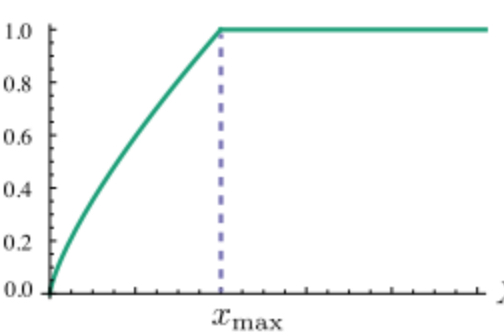
\includegraphics[width=2.5in]{figures/glove1.png}
\caption{Glove权重函数}\label{fig:glove1}
\end{center}
\end{figure}

\begin{table}[h]
	\centering
	\scalebox{0.9}{
		\begin{tabular}{l|llllll}
		  \toprule
		  \midrule
		                &我 &爱 &喜欢   &飞机   &自然语言处理   &深度学习\\
		  \midrule
		    我          &0  &2  &1      &0      &0              &0\\
		    爱          &2  &0  &0      &0      &1              &1\\
		    喜欢        &1  &0  &0      &1      &0              &0\\
		    飞机        &0  &0  &1      &0      &0              &0\\
		    自然语言处理&0  &1  &0      &0      &0              &0\\
		    深度学习    &0  &1  &0      &0      &0              &0 \\
		  \bottomrule
		\end{tabular}
	}
	\caption{共现矩阵}  
	\label{tab:comatrix}
\end{table}
我通过一个例子来讲解共现矩阵的构造方法,假定存在一个语料库,这个语料库比较简单,以方便我们能够更好解释问题。语料库比较简单,只有三个句子:(1)我 爱 深度学习;(2)我 爱 自然语言处理;(3)我 喜欢 飞机。这个语料库中总共有6个词——我、爱、喜欢、飞机、自然语言处理和深度学习。对于“我”字其共现的词语是“爱”(2次)、“喜欢”(1次);对于“爱”其共现词语是“我”(2次)、“喜欢”(1次)、“深度学习”(1次)和“自然语言处理”(1次);对于“喜欢”其共现词是“我”(1次)、“飞机”(1次);对于“飞机”其共现词是“我”(1次);对于“自然语言处理”其共现词是“爱”(1次);对于“深度学习”其共现词是“爱”(1次)。根据共现关系我们可以通过下面的方法来构建共现矩阵$C=\{c_{i,j}|i,j=1,2,\cdots,n\}$。$c_{i,j}$表示编号为$i$的元素为中心词,编号为$j$
的词的出现次数。对于上面的例子我们构造出来的共现矩阵如\ref{tab:comatrix}表所示。这样上面公式推导中的$p(w_j|w_i)=\frac{c_{i,j}}{\sum_{k=1}^{n}{c_{i,k}}}$。


\subsection{词向量的评估方法}
词向量的训练可以被认为是一种无监督的方法,如何评价词向量对语意的表示质量,是一个有挑战的任务。
Schnabel 最先做这方面的系统性研究,他将词向量的评估方法分成两方面——内涵评估和外延评估:

$-$ \textbf{外延评估}
 
这种评估方法就是将词向量作为下游任务的初始词向量,观察词向量能否改善下游任务的关键指标。比如能够帮助文本分类、\gls{NER}等任务的准召率。由于外延评估不是直接评估,而是假设好的词向量一定能够帮助下游任务提升指标这一并不一定成立的指标,存在下游模型和词向量相互拮抗的可能,因此通常会作为间接评估使用。但大量的研究表明现有的词向量训练方法都能够和主流的下游模型协同作用。

$-$ \textbf{内涵评估}

在内涵评估(intrinsic evaluation)中,可以观察词向量承载了多少词之间语义上的联系。做内涵评估通常需要一个查询库(query inventory),同时需要一些人工标注。内涵评估可以分成两类,但是这两类方法都是为比较不同方法训练出的词向量而设计,尤其是比较评估法是直接让人来选哪种词向量更容易接受,因此这里暂时不做讨论;绝对评估法是对每种词向量单独评估,又可以划分为四项评估方式
\begin{description}
\item [相关性(relatedness)]对于一对相关度比较高的词,其预先相似度也要高,这里作为标准的相关度评分由人工给出。
\item [类比性(analogy)]对给定的词y,能否找到一个对应的词x,使x与y的关系能够类比另两个已知词a与b之间的关系。例如比较经典的king-queen与man-woman之间的关系
\item [类别化(categorization)]对词向量进行聚类,看每个簇与有标记数据集各类相比纯度如何
\item [选择倾向(selectional preference)]判断某些名词是更倾向做某个动词的主语还是宾语,例如一般顺序是people eat而不是eat people
\end{description}

最后,可以参考GitHub上一套公开的benchmark,这个仓库不仅提供了评估代码,也提供了原始数据集做检查
\chapter{语言模型}
\section{语言模型的定义和句子通顺度评估}
\begin{definition}
对于一个给定的句子$S=s_1,s_2,\cdots ,s_N$,语言模型给出的数学形式是在前文$n$个词确定的条件下,下一个词汇的分布概率:
$$
p(s_{n+1}|s_1,s_2,\cdots,s_n)
$$
如果给定的前文长度为$n$,那么这个语言模型被称为$n$-gram语言模型。
\end{definition}

语言模型一个简单的应用是用来评价一个给定的句子$S=s_1,s_2,\cdots ,s_N$是不是符合语法要求或者说是否通顺的。那么如何使用语言模型给一个句子的通顺度打分呢?假定我们有一个训练好的$n$-gram语言模型语言模型和一个给定的句子$S=s_1,s_2,\cdots ,s_N$,那么这个句子的通顺$\gamma(S)$程度可以使用下面的公式来近似:
$$
\gamma(S) = -\frac{\sum_{i=n, n+1, \cdots, |S|}log(p(s_{n+1}|s_1,s_2,\cdots,s_n))}{|S|-n}
$$
这个公式可以理解为平均到句子的单个词汇中,其在窗口为$n$的上下文中,平均出现概率。显然句子越通顺,这个句子的滑动窗口下一个词出现的概率应该越高,因此这个平均概率也越大。如果我们稍微变化一下就是语言模型的困惑度的概念:
$$
PPL(S) =2^{ -\frac{\sum_{i=n, n+1, \cdots, |S|}log_2(p(s_{n+1}|s_1,s_2,\cdots,s_n))}{|S|-n}}
$$
\section{前馈神经网络语言模型}
在神经网络兴起之前,人们通常使用频率估计的方法来构建语言模型,为了应对其中的不平滑性,人们想出了各种各样的插值方法。现有的历史文献中,还有对插值平滑的大量讨论,但是随着神经网络技术的发展,插值技术由于缺乏足够的数学原理支持,更多的是使用经验,因此慢慢地被人们遗忘。除了自然语言处理中的不平滑性,另外一个严重的问题是维度诅咒,举个例子,如果词表大小是10000,一个$n$-gram 语言模型的参数量是$~10000^n$。这个一个难以让人接受的数据规模,事实上汉语的词汇量远不止这个量级,为此很多研究人员将$n$-gram 语言模型参数随着词表快速膨胀的问题称之为维度诅咒。

新兴的技术已经可以用更为简洁的方法在一定程度上解决了统计语言模型的维度膨胀等一些列问题了,这一切的进展主要受益于神经网络的快速发展。据我们所知,第一个神经网络语言模型出自著名的计算机学家Benjio之手。Benjio在2003年提出了第一个基于神经网络的语言模型,这个模型首先将前$n-1$个窗口词汇用one-hot编码之后$X_t=[x_{t-1},\cdots,x_{t-2},x_{t-n+1}]$, 通过乘以一个可训练的共享矩阵$E=[e_{i,j}|i=1,2,\cdots,|V|;j=1,2,\cdots,h]$,得到一个$n \times H$的矩阵$\hat X_t=EX_t$,并通过$tanh$激活函数得到隐层的输出$H$:
$$
H = tanh(d + W_1EX_t)
$$
$H$和$\hat X$的分别通过两个参数不同线性投射层后,做加权和去预测当前词出现的概率:
$$
p(x_t|x_{t-1},\cdots,x_{t-2},x_{t-n+1}) = softmax(b+W_3EX_t+W_2H) 
$$
这里所谓共享是指不同的句子不同的窗口都使用同样的矩阵,这个矩阵是随机初始化的,我把它称之为随机词向量矩阵,通过梯度下降来学习。网络的结构如图\ref{fig:nnlm}所示。

\begin{figure}[h]
\begin{center}
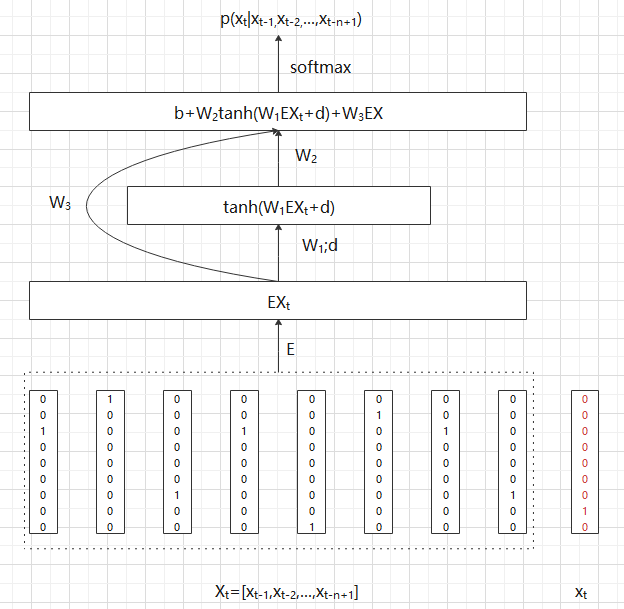
\includegraphics[width=5.5in]{figures/nnlm.png}
\caption{前馈神经网络语言模型} \label{fig:nnlm}
\end{center}
\end{figure}

前馈神经网络语言模型在一定程度上解决了统计语言模型的不平滑性和维度膨胀问题,但是并没有考虑窗口内部词语的顺序,但是这项研究催生了上一节我们提到的\gls{CBOW} 词向量技术的诞生。另外为了将窗口内部词语的顺序能够建模到语言模型的语意捕捉框架里,基于循环神经网络的语言模型也渐渐兴起。前馈神经网络是神经网络在自然语言处理领域最具影响力的研究,是神经网络自然语言处理技术的里程碑式的研究成果,开启了人工神经网络自然语言处理的新赛道,是具有奠基意义的重要成果。

\section{循环神经网络语言模型}
\subsection{循环神经网络}
循环神经网络的研究发端于上世界八九十年代,在1990年,Jeffrey Elman提出了第一个全连接的\gls{RNN}所以这个网络也被称为Elman网络。Elman 网络的结构如图\ref{fig:rnn1}所示,除了输入层(其输入为$X$,输出为$\hat X$)和输出层(其输入为$\hat Y$,输出为$Y$),循环神经网络存在一个随着序列推进动态更新的隐藏层(其隐藏状态为$S$):

\begin{figure}[htbp]
\begin{center}
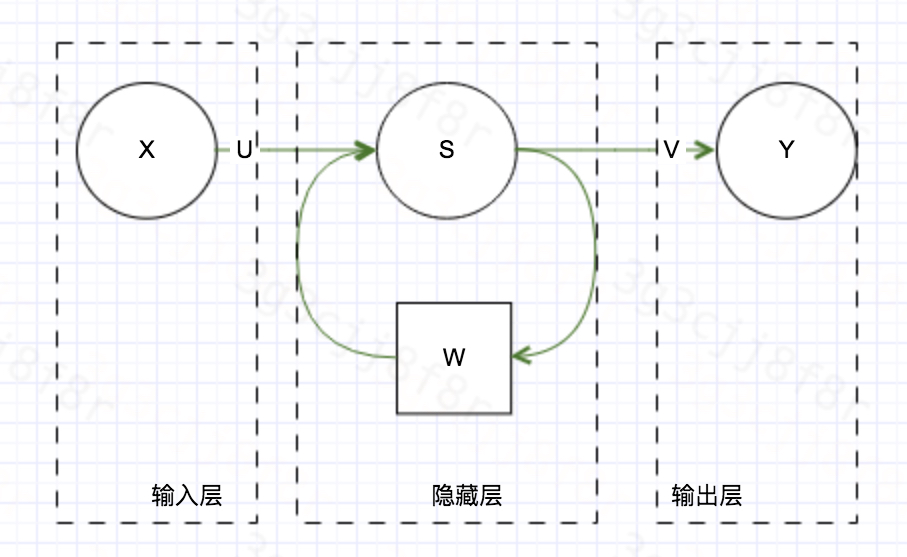
\includegraphics[width=5.0in]{figures/rnn1.png}
\caption{循环神经网络}\label{fig:rnn1}
\label{default}
\end{center}
\label{rnn1}
\end{figure}

循环神经网络的计算流程如下:
$$
\begin{aligned}
\hat{X_t} =& UX_t \\
\hat Y_t =& f(\hat X_t + WS_{t-1}) = f(UX_t + WS_{t-1}) \\
Y_t=&g(V\hat Y_t) =g(Vf(UX_t + WS_{t-1})) 
\end{aligned}
$$
另外,隐藏层也会随着时间的迭代逐步更新:
$$S_t = l(WS_{t-1})$$

随着梯度下降后向传播算法在其他领域的成功,人们开始尝试将梯度下降后向传播算法应用到循环神经网络中去,差不多在Elman网络被提出的前一年,Paul Werbos提出了随时间反向传播的梯度下降算法——BPTT,因此人们开始去挖掘循环网络的应用,可悲的是人们很快发现了两个要命的问题,对于长序列BPTT算法会引入梯度消失和梯度爆炸问题。所谓梯度消失或者梯度爆炸问题,简单来说就是按照链式求导法BPTT算法中会按照时间展开,但是由于其中间项太多导致梯度随着时间传播可能会变得极小或者极大,从而导致训练的不稳定。任何网络都不能从理论上证明必然出现梯度消失或者梯度爆炸的,但是人们在训练神经网络的过程中,有些网络比较大概率被观察到了模型梯度变成0导致参数不更新,形成吸收态,通常人们就会说这个网络有梯度消失问题;反之如果经过链式规则后,有些网络比较大概率被观察到的梯度值非常大,导致后续学习出现大幅度的波动,从而导致模型性能下降,甚至不收敛,通常人们就会说这个网络有梯度爆炸问题。不幸的是
循环网络就被观察到了梯度消失和梯度爆炸问题,特别是在建模的序列长度超过20的时候。于是人们开始了与梯度消失和梯度爆炸的对抗,人们发现解决梯度爆炸问题有一个非常暴力的方法——梯度裁剪,所谓梯度裁剪就是当梯度值非常大的时候人们给他削顶,这个算法非常简单粗暴,但是效果却出奇的好。
这里我们给出在tensorflow 框架下实现梯度裁剪的一个样例代码:
\begin{lstlisting}[language={python}]

def noam_scheme(init_lr, global_step, warmup_steps=4000.):

    step = tf.cast(global_step + 1, dtype=tf.float32)
    return init_lr * warmup_steps ** 0.5 * tf.minimum(step * warmup_steps ** -1.5, step ** -0.5)
    
def create_train_opt_with_clip(loss, step_num_in_epoch=1000):

    global_steps_ = tf.train.get_or_create_global_step()
    global_step = tf.cast(x=global_steps_, dtype=tf.float32)
    learning_rate = noam_scheme(init_lr=0.003, global_step=global_step)
    admw = tf.contrib.opt.extend_with_decoupled_weight_decay(tf.train.AdamOptimizer)
    optimizer = admw(weight_decay=0.0001, learning_rate=learning_rate)
    grads, variables = zip( * optimizer.compute_gradients(loss))
    grads, global_norm = tf.clip_by_global_norm(grads, 5.0)
    train_op = optimizer.apply_gradients(grads_and_vars=zip(grads, variables), global_step=global_steps_)
    return train_op, learning_rate
 \end{lstlisting}
 
 梯度消失问题的解决是非常有挑战的,当梯度变得很小的时候,模型的参数随之更新也会变得非常小,因此这些参数不在变化,从而形成恶性循环。最有影响力的研究是Long short-term memory, \gls{LSTM},这个网络的精妙之处是增加了若干门控,从而极大缓解了\gls{RNN}原始网络中的梯度消失问题。\gls{LSTM}的网络结构如图\ref{fig:lstm1}所示。
\begin{figure}[htbp]
\begin{center}
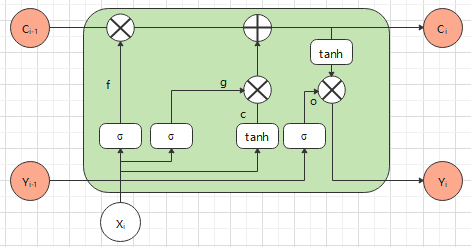
\includegraphics[width=4.5in]{figures/lstm1.png}
\caption{长短记忆网络}\label{fig:lstm1}
\end{center}
\end{figure}  
\gls{LSTM} 在训练的时候参数因为每个时刻的输出依赖前一时刻的隐藏层状态,因此并行化程度较低,无法充分利用GPU带来的并行计算能力。人们为了降低\gls{LSTM} 的复杂度,引入了\gls{GRU}模型,\gls{GRU} 可以认为是\gls{LSTM}的简化版本。

由于\gls{LSTM} 的出现,原来的梯度消失和梯度爆炸问题得到很大程度上缓解,注意这里讲的是缓解并不是解决。很多模型训练的时候,还是会使用梯度裁剪技术防止梯度爆炸,特别是在使用多层\gls{LSTM}模型的时候;另外在训练多层\gls{LSTM}的时候通常会使用残差连接来避免梯度消失。著名的基于多层\gls{LSTM}的机器翻译模型就使用了上述两个技术。另外使用\gls{LSTM}的时候人们观察到一个有趣的现象,逆序输入句子到循环神经网络会比正序输入句子到循环神经网络,效果要好很多,大家不妨在自己的工程实践中尝试一下。

\subsection{循环神经网络语言模型}
循环神经网络语言模型最早由Bengio 在2003年提出FFNNLM的时候,就提到了使用\gls{RNN}来训练语言模型的想法,但是第一个基于\gls{RNN}的神经网络语言模型出现在2010年,Mikolov 提出了基于循环神经网络的语言模型,在PPL指标上取得突破性进展。Mikolov 在训练语言模型的时候用到了teacher-forcing 模式。\gls{RNN}在训练语言模型的时候通常会针对一个句子构建一对平行语料。平行语料的源语句就是这个句子之前增加一个特殊字符“[Start]”,比如给定的句子是“我 是 一个 热爱 自然语言处理 的 工程师”,那么经过处理的源句子会变成,“Start 我 是 一个 热爱 自然语言处理 的 工程师”;平行语料的目标语句会在句子之后增加一个特殊字符“[Stop]”,比如上述句子的目标语句就是“我 是 一个 热爱 自然语言处理 的 工程师 [Stop]”。下表的第一行是序列时刻,第二行和第三行分别是模型的源语句和目标语句。
\begin{table}[h]
	\caption{语言模型数据处理}  
	\label{tab:schedule}
	\centering
	\scalebox{0.9}{
		\begin{tabular}{lllllllllll}
		  \toprule
		  \midrule
		  &&1&2&3&4&5&6&7&8\\
		   源语句$X$ & & [Start]& 我& 是& 一个& 热爱& 自然语言处理 &的 &工程师\\
		   目标语句$Y$ & & 我& 是 &一个 &热爱 &自然语言处理 &的 &工程师 &[Stop] \\
		  \bottomrule
		\end{tabular}
	}
\end{table}
\subsubsection{循环神经网络的两种训练模式}
循环神经网络(\gls{RNN}) 在语言模型训练的时候有两种模式:free-running 模式和teacher-forcing 模式。这两种模式的区别在于$t$时刻的输入$x_t$是不是$t-1$时刻的解码输出。如果是前一个时刻的解码输出,那么\gls{RNN}就处于free-running模式;如果不是$t-1$时刻的解码输出而是$t$时刻目标语句对应的词$y_{t}$,作为\gls{RNN}的当前输入,那么\gls{RNN}处于teacher-forcing 模式。teacher-forcing 模式的优点是实现起来比较容易,而且通过$t$时刻目标语句对应的词$y_{t}$作为输入,避免了解码造成的误差传递,降低了训练的难度;当然由于直接使用了$y_{t}$作为$t$时刻的输入,所以切断了学习解码噪声的机会。目前工业界和学术界,基本上都在使用teacher-forcing 模式训练\gls{RNN}模型。

\begin{figure}[htbp]
\begin{center}
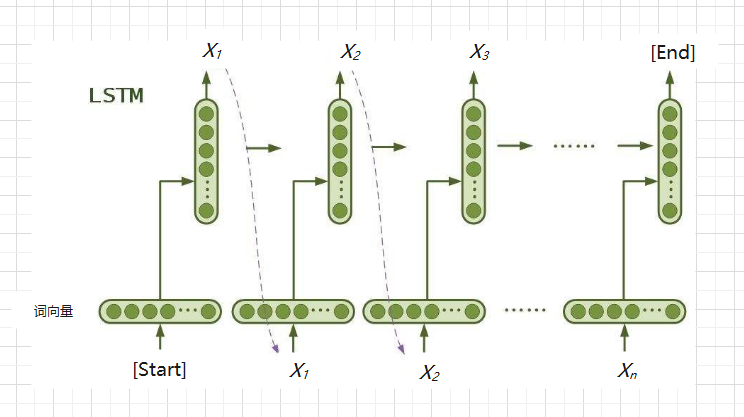
\includegraphics[width=5.5in]{figures/rnnlm1.png}
\caption{循环神经网络语言模型结构}\label{fig:rnnlm1}
\end{center}
\end{figure}

\subsubsection{循环神经网络语言模型的模型细节}
循环神经网络(\gls{RNN})语言模型的结构如图\ref{fig:rnnlm1}所示,模型通过$t$时刻的\gls{RNN}的输出通过softmax层后的预测值为$\hat y_t$用于表示模型对于$p(x_t|x_{<t})$的估计。\gls{RNN}语言模型认为语料库中的自然形成的句子都是非常通顺的,对于一个给定的句子$X = x_1,x_2,\cdots, x_n$,那么一个训练良好的网络模型,$p(x_t=y_t|x_1=y_1,x_2=y_2,\cdots, x_{t-1}=y_{t-1})$的概率应该最大。其损失函数应该是
$$
\begin{aligned}
J(\theta) = & \sum_{t=1,2,\cdots,n}{-log(\hat y_t) \varepsilon (y_t)}
\end{aligned}
$$
其中$\varepsilon(y_t)$表示$y_t$的one-hot编码。\gls{RNN}单元可以是原始的\gls{RNN}单元、\gls{LSTM}单元或者\gls{GRU}单元。研究表明他们混淆度指标排序是\gls{RNN}<\gls{GRU}<\gls{LSTM}。下面我们给出一个基于tensorflow的实现:
\begin{lstlisting}[language={python}]
class LSTMLM:
	
	def __init__(self, x_id, x_mask, y_id, config, mode):
		
		self._x_id = x_id
		self._x_mask = x_mask
		self._y_id = y_id
		self._config = config
		self._mode = mode
		self._loss = None
		self._softmax = None
	
	def create_model(self):
		input_shape_list = get_shape_list(self._config)
		# 1. embedding layer
		emb_table = tf.get_variable(name='embedding',
		                shape=[self._config.vocab_size, self._config.hidden_size],
		                initializer=tf.contrib.layers.xavier_initializer())
		
		x_emb = tf.nn.embedding_lookup(params=emb_table, ids=self._x_id)
		
		# 2. rnn layer
		cell = tf.contrib.rnn.BasicLSTMCell(self._config.hidden_size)
		cell.zero_state(input_shape_list[0], dtype=tf.float32)
		output_keep_prob = self._config.keep_prob if self._mode == tf.estimator.ModeKeys.TRAIN else 1.0
		lstm_cell = tf.contrib.rnn.DropoutWrapper(cell, output_keep_prob=output_keep_prob)
		
		# B x S x H
		outputs, last_states = tf.nn.dynamic_rnn(cell=lstm_cell, inputs=self._x_id,
		                  sequence_length=tf.reduce_sum(input_tensor=self._x_mask, axis=-1, keep_dims=False))
		# 3. project layer
		logits = tf.layers.dense(inputs=outputs, units=self._config.vocab_size, activation=tf.nn.relu, use_bias=True)
		self._softmax = tf.nn.softmax(logits=logits, axis=-1)
		
		return logits
	
	def get_prediction(self):
		
		return self._softmax
	
	def get_loss(self, logits):
		
		# B x S
		loss_per_sample = tf.nn.sparse_softmax_cross_entropy_with_logits(labels=self._y_id, logits=logits)
		loss_per_sample_after_mask = loss_per_sample * tf.cast(x=self._x_mask, dtype=tf.float32)
		loss = tf.reduce_mean(loss_per_sample)
		self._loss = loss
		
 \end{lstlisting}
 \section{卷积神经网络语言模型}
 \subsection{卷积神经网络}
 计算机学家对卷积神经网络的研究,开始于二十世纪80至90年代,最早人们用卷积的伸缩平移不变性,来解决音频和图像等领域的问题。比较有影响力的研究成果是Yann LeCun在1989年构建的应用于计算机视觉问题的卷积神经网络,这个神经网络就是后来大名鼎鼎的LeNet的最初版本。LeNet 在手写数字识别领域取得了巨大的成功,极大鼓舞了人们讲神经网络技术应用到计算机图像学领域。图\ref{fig:lenet1}就是LeNet大体结构。
\begin{figure}[htbp]
\begin{center}
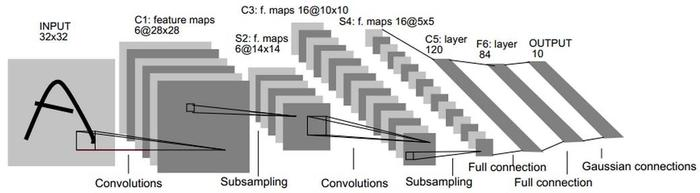
\includegraphics[width=5.5in]{figures/lenet1.jpg}
\caption{LeNet网络结构}\ref{fig:lenet1}
\end{center}
\end{figure}

这个网络的feature maps 层也被称为卷积层,我们先来介绍一下卷积操作,对于单通道图像,卷积操作如图\ref{fig:cnn}所示.
\begin{figure}[htbp]
\begin{center}
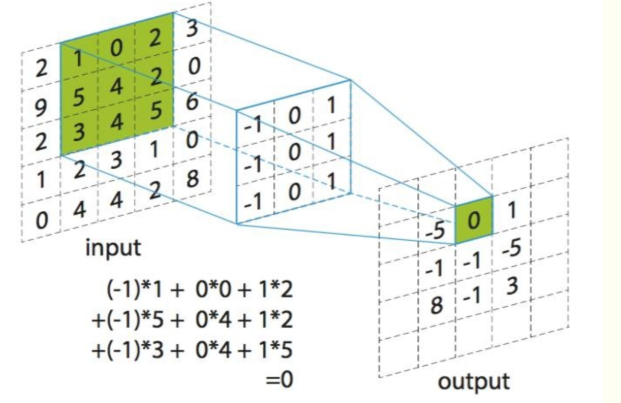
\includegraphics[width=5.5in]{figures/cnn.png} 
\caption{CNN 计算流程}\label{fig:cnn}
\end{center}
\end{figure}
假定卷积核为$F=\{f_{i,j}|i=1,2,\cdots,K;j=1,2,\cdots,L\}$, 输入的单通道图像为$X=\{x_{i,j}|i=1,2,\cdots,N;j=1,2,\cdots,M\}$,那么输出的结果为
$$
y_{i,j} =\sum_{k=1}^{K}\sum_{l=1}^{L}x_{i+k,j+l}*f_{k,l} 
$$
如果是多通道图片,例如包含RGB三个通道,那么卷积核就必须包含三个通道,相当对三个通道同时做单通道卷积,然后对应位置求和。假定各个通道的卷积结果分别为
$$
\begin{aligned}
y^{R}_{i,j} &=\sum_{k=1}^{K}\sum_{l=1}^{L}x^{R}_{i+k,j+l}*f^{R}_{k,l}\\
y^{G}_{i,j} &=\sum_{k=1}^{K}\sum_{l=1}^{L}x^{G}_{i+k,j+l}*f^{G}_{k,l}\\
y^{B}_{i,j} &=\sum_{k=1}^{K}\sum_{l=1}^{L}x^{B}_{i+k,j+l}*f^{B}_{k,l} \\
\end{aligned}
$$
那么最终的输出结果就是各个通道的和
$$
y_{i,j}=y^{R}_{i,j} + y^{G}_{i,j} + y^{B}_{i,j}
$$

LeNet 网络中有一个Subsampling层,这个层也被称为池化层,用来减少模型的参数,在上世纪,LeNet 必须能够降低自己的参数量从而减低计算量,这样CPU才能执行BP算法。但是随着计算机技术的进步,特别是GPU性能的大幅提升,人们不仅没有把池化层去掉反而发现了它的一些其他精妙之处:
\begin{description}
\item [特征挑选]池化操作使得模型更加关注是否存在某些特征而不是特征具体的位置,不过也有的学者对此提出了不同看法,Hinton 提出的胶囊网络就重新把特征的位置建模到了模型中。
\item [特征降维]经过池化层之后,模型的输入变小,便于人们训练深层的模型,进行更抽象的特征抽取,目前的一些图像识别算法的深度都达到了惊人的几十层之多。
\item [提升泛化性]由于降低了参数的数量,因此在一定程度上防止过了拟合。
\end{description}

\subsection{门控卷积神经网络语言模型}
由于神经网路语言模型的训练是非常耗时的一件事情,训练一个隐藏层为1024维的循环网络语言模型,需要花费32张GPU近三周的时间。毫无疑问人们热切的希望加速算法的出现,\gls{CNN}作为一种天然适合GPU并行处理的网络,受到了Facebook 公司的研究人员的注意,他们设计了一个称为门限\gls{CNN}的神经网络语言模型,研究者宣称他们在同样的数据集中使用\gls{CNN}技术,用1张同等规格的GPU,仅花费2周时间就训练出困惑度更低的语言模型,让人们看到\gls{CNN}的独特用处和强大威力。门控卷积神经网络的数据处理跟循环神经网络语言模型相同,都是会针对一个句子构建一对平行语料。平行语料的源语句就是这个句子之前增加一个特殊字符“[Start]”,平行语料的目标语句会在句子之后增加一个特殊字符“[Stop]”。

门控神经网络的输入句子经过one-hot 编码后得到平行语料的源语句数学表示$X=[w_1,w_2,\cdots,w_N]$,然后乘以随机初始化的词向量矩阵$D^{|V| \times h}$,得到第一个隐藏层的输入$E_{1}=[D_{w_1},D_{w_2},\cdots,D_{w_N}]$。上面的$V$是我们的词表,$|V|$表示词表的大小。我们通过下面的门控卷积神经单元运算得到第一个隐藏层的输出,作为下一个隐藏层的输入
$$
E_{i+1} = (f(E_i; W_i) + b_i) \otimes \sigma(f(E_i; V_i) + c_i)
$$
其中$\sigma$ 表示sigmoid 函数,$\otimes$ 表示对应位置相乘,$f(X;K)$ 表示卷积运算,$K\in R^{k \times n \times n}$表示卷积核,通常需要合理设计卷积的PADING和卷积核的尺寸,并对输出矩阵执行适当的形状变换,保证输入和输出的矩阵形状不变。如图所示,我们可以使用$N$个尺寸为 $k \times n$卷积核,并对输入的句子句首PADING $k-1$个$1 \times n$的$0$向量,然后从左到右执行卷积操作。

\begin{figure}[htbp]
\begin{center}
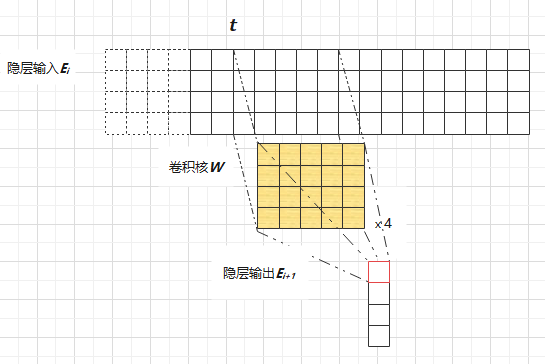
\includegraphics[width=5.5in]{figures/cnnlm1.png}
\caption{CNN 语言模型的处理流程}
\label{fig:cnnlm1}
\end{center}
\end{figure}
另外,最后一个隐藏层的输出会直接通过线性投射层后执行softmax计算其损失或者作为预测的概率分布,网络的详细结构如图\ref{fig:cnnlm2}所示。
\begin{figure}[htbp]
\begin{center}
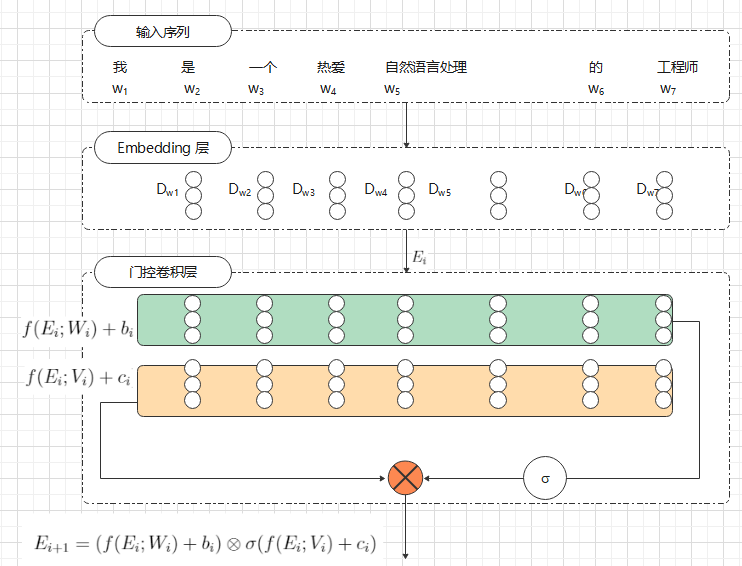
\includegraphics[width=5.6in]{figures/cnnlm2.png} 
\caption{门控卷积神经网络语言模型}\label{fig:cnnlm2}
\end{center}
\end{figure}

门控卷积神经网络是对卷积神经网络的一种改进,模型在学习特征抽取的同时,学习抽取到特征筛选过程,从提高了模型的泛化能力。这种想法与\gls{LSTM}对传统\gls{RNN}的改进如出一辙,论文的作者也做了类比。类似于\gls{LSTM},作者发现门控卷积神经网络能从理论上缓解梯度消失现象。另外作者在训练的时候使用自适应softmax替代传统的softmax 来加速训练过程。

\section{自注意力神经网络语言模型}
注意力机制在自然语言处理领域的应用缘起于人们对机器翻译的研究,从直觉看来,目标语言的生成过程中,特定字的挑选通常与源语言中某些字有重要联系,而与其他的字关系相对较小,为此人们希望在生成指定位置的模型语言输出的时候,能够将注意力集中到源语言的某些关键词中而不是全部词汇。这就是注意力机制的基本内涵,事实上,同一个句子的不同部分通常也是有联系的,而且不同部分之间的联系程度彼此也不相同。人们发现同一个句子彼此之间的注意力建模,能够建模不同词语之间的语义联系,极大的改善了机器翻译的质量。后来人们将机器翻译源语句建模的思路用到了训练神经网络语言模型中,极大的降低了测试集的混淆度,而且在很大程度上扩展了神经网络语言模型在文本生成领域的应用。关于注意力机制在机器翻译领域的应用,我们会在后续的章节中详细介绍。

\subsection{自注意力机制}
假定有两个句子,他们分别是中文和英文,表达了同样的意思,都在说”我是一个热爱自然语言处理的工程师“。我们知道中文属于蒙藏语系,是表形文字,例如”月“字的甲骨文写法,可以清楚的看出来是一弯月亮;而英文属于印欧语系,每个词由若干字母按照顺序组成,是表音文字,例如”moon“的英文写法,我们基本可以推测出这个词的发音。中文在表达”我是一个热爱自然语言处理的工程师“的时候,用了一系列的表形符号;英文在表达同样的意思的时候,用了一系列的表音符号。如下表\ref{tab:zh_en}所示
\begin{table}[h]
	\caption{中英文表意对比}  
	\label{tab:zh_en}
	\centering
	\scalebox{0.9}{
		\begin{tabular}{lll}
		  \toprule
		  \midrule
		  英文 & & I am a engineer who loves natural language processing very much\\
		  \hline
		  中文 & & 我,是,一个,热爱,自然语言处理,的,工程师\\
		  \bottomrule
		\end{tabular}
	}
\end{table}
那么如何构建出上述两个句子之间的关系呢?通常的做法是,首先找到中英文句子的数学表示(通常是矩阵,我们将其分别记作$Q=[Q_1,Q_2,\cdots,Q_N]$和$K=[K_1,K_2,\cdots,K_M]$),其中$Q_i$或者$K_j$ 是一个一维的矩阵分别表示源语言和目标语言的一个词,可以是预训练的词向量。

我们知道在线性代数里,一个向量可以理解为多维线性空间中的一个点,那么两个向量之间的关系如何建模呢?数学上有很多种表示方法,注意力模型中最常用的方法是使用向量的点乘来表示两个空间中点的关系。假定在高维空间中存在一组向量$K=[K_1,K_2,\cdots,K_n]$,且$K$ 中的向量线性无关,对于某个向量$Q_i$, 那么$softmax(Q_iK^T)K$就可以近似表示,$Q_i$在$K$向量组张成的线性空间中的位置。由于句子中的每个位置的词通常是不同的,即使是相同但是由于其位置不同其表意也会有差异,因此基本可以认为一个句子中的各个词向量是彼此线性无关的。这样一来,$Q_i$和$K$向量组中哪个向量关系大,那么对应$softmax(Q_iK^T)$对应的维度就越大。可以说注意力机制将两种不同方式的表示统一到同一个数学空间中去进行计算,因此构建了同一语义不同形式表达的计算关系。事实上,很多研究者通过不同侧面的大量实验都证明了这种关系构建方法的有效性。

在自然语言处理中,  $K$通常是一个句子,如上述平行语料中的源语句,其中每个子向量$K_i$都表示一个句子的词汇,$Q_i$ 代表另一个句子中的一个词汇,因此注意力机制可以在向量组$K$代表的语义空间中测量$Q_i$和$K_1,K_2,\cdots,K_n$的语义关系。如果$Q_i$ 是句子$K$中的任意一个词,那么可以度量在$K$代表的语义空中各个元素的相互语义关系。显然前$t$个词彼此之间的相互语义关系建模,在根据句子的前$t$个词来预测第$t+1$词分布的任务中有积极意义,于是人们设计出了自注意力语言模型:\gls{GPT}。

\subsection{GPT-自注意力神经网络语言模型}
自注意力神经网络语言模型的出现是受益于自注意力机制在机器翻译领域的巨大成功。2018年google公司的研究人员发表了一篇题为《Attention is all your need》的论文,提出了一种全新的文本特征提取方法,并改善了机器翻译的质量,因此引起了学术界和工业界的高度关注,后来的\gls{BERT}和\gls{GPT}都是基于这项研究做出来的。通常人们将《Attention is all your need》 提出的方法称为Transformer,我们会在后续的章节详细介绍Transformer的结构。这里仅仅介绍一下它的大致结构,从宏观上看Transformer由几乎对称的两个部分组成:编码器和解码器。编码器使用多层自注意力结构构建机器翻译源语句的语义表示,解码器使用多层自注意力结构构建目标语句的语义表示的同时利用注意力机制建立目的语句表示和源语句表示的语义关系。Transformer模型的大致结构如图\ref{fig:gpt1}所示。
\begin{figure}[htbp]
\begin{center}
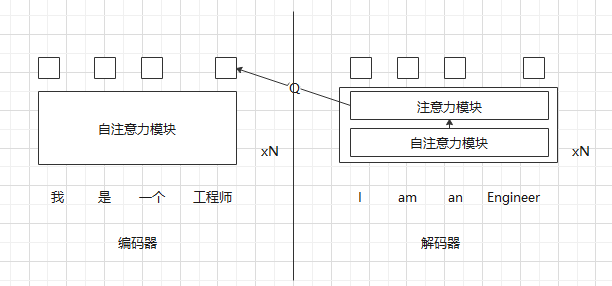
\includegraphics[width=5.5in]{figures/gpt1.png}
\caption{Transformer网络结构}\label{fig:gpt1}
\end{center}
\end{figure}
\gls{GPT} 模型就是摘取了Transformer的编码器,并改造了其中的自注意力模块,保证当前词语的注意力不会放到当前词的右边,保证了因果性,并且给编码器增加了一个用于训练语言模型的损失函数。值得注意的是\gls{GPT}通过海量的非监督语料的长时间训练,取得了广受瞩目的成绩,甚至不少媒体对其进行了报道,不过\gls{GPT}就是Transformer的Encoder的因果性改造后通过传统语言模型训练损失得来的。

由于这个模型相对复杂,我们一步一步来讲解\gls{GPT}基于Tensorflow的实现过程。首先定义文本输入和label,其中x\_placeholder是文本的ID序列,x\_mask\_placeholder是文本ID序列的有效位置,一般来说,x\_placeholder的每一个句子的长度通过补零得到一个长度为max\_seq\_len的整数数组,因此需要通过x\_mask\_placeholder来表明哪些位置是有效的位置(mask数组对应位置值为1),哪些位置是补零的位置(mask数组对应位置值为0)。另外在语言模型训练中通常会对输入序列前补一个特殊字符(我们记为[START])表示句子的开始,并在label序列的最后补一个特殊字符(我们记为[END])表示句子的结束。
\begin{lstlisting}[language={python}]
import tensorflow as tf
x_placeholder = tf.placeholder(dtype=tf.int32, shape=[batch_size, max_seq_len], name='x')
x_mask_placeholder = tf.placeholder(dtype=tf.int32, shape=[batch_size, max_seq_len], name='x_mask')
y_placeholder = tf.placeholder(dtype=tf.int32, shape=[batch_size, max_seq_len], name='y')
\end{lstlisting}
接下来就是Embedding处理了,具体的处理方法如下面的代码,主要是将ID的随机Embedding和位置随机Embedding直接加在一起。
\begin{lstlisting}[language={python}]
# output x
embedding_lookup_tbl = tf.get_variable(name='embedding_lookup_tbl',shape=[vocab_size,hidden_size],dtype=tf.float32,	initializer=tf.contrib.layers.xavier_initializer())
pos_embedding_lookup_tbl_decoder = tf.get_variable(name='embedding_lookup_tbl',shape=[max_pos_size,hidden_size],dtype=tf.float32,initializer=tf.contrib.layers.xavier_initializer())
x_id_emb = tf.nn.embedding_lookup(params=embedding_lookup_tbl, ids=x_placeholder)
x_id_emb *= get_shape_list(x_id_emb)[-1] ** 0.5
# position embedding
seq_len = get_shape_list(x_id_emb)[1]
x_position_emb = tf.slice(input_=pos_embedding_lookup_tbl_decoder, begin=[0, 0], size=[seq_len, -1])
x_position_emb = x_position_emb * tf.cast(x=tf.expand_dims(input=x_mask_placeholder, axis=-1), dtype=tf.float32)
x = x_id_emb + x_position_emb	# B x S x H 最后的输出
\end{lstlisting}
后面对接的是多层因果自注意力模块,这里涉及到了因果多头注意力机制,具体来说就是在求自注意力的时候避免当前词和这个词的右边词汇的词向量发生关系,这里我们使用了一个技巧,通过给Attention权重矩阵加上一个非常小的负数,然后这个操作会使得这个Attention矩阵经过softmax之后变成一个三角矩阵从而保证因果性,这里使用scaled\_dot\_product\_attention这个函数的时候其中attention\_future这个参数被设置成了False。后面我们会详细介绍Transformer的实现细节,这里大家只要关注如何在多头注意力上添加因果约束就好了。
\begin{lstlisting}
# input x和x_mask_placeholder
# output x_ret
def add_and_norm(x, y, scope):
	# HERE DIFFERENT FROM PAPER
	ret = y + x
	ret = layer_normalize(inputs=ret, scope=scope)
	return ret

def scaled_dot_product_attention(k, q, v, mask_k, mask_q, mask_v,attention_size, attention_dropout, training=True, attention_future=True):
		def attention_mask_before_softmax(matrix, from_mask, to_mask, attention_future=True):
			to_mask = tf.cast(x=to_mask, dtype=tf.float32)
			attention_adder = (1.0 - tf.expand_dims(input=to_mask, axis=1)) * (-2.0**31+1.0)

			if attention_future == False:
				mask_matrix = tf.ones_like(matrix[0], dtype=tf.float32)
				mask_matrix = 1.0 - tf.linalg.band_part(input=mask_matrix, num_lower=-1, num_upper=0)
				mask_matrix = tf.expand_dims(input=mask_matrix, axis=0) * (-2.0**31+1.0)
				matrix = matrix + mask_matrix # here the first dimision will be broadcast

			return matrix + attention_adder	# here attention_adder will be broadcast according to axis 1
			
		# QK^T
		dot_product = tf.matmul(a=q, b=k, transpose_b=True)
		# scale
		dk = tf.cast(x=attention_size, dtype=tf.float32)
		scale_dot_product = dot_product / tf.sqrt(dk)
		# mask & softmax
		scale_dot_product = attention_mask_before_softmax(matrix=scale_dot_product,
																						from_mask=mask_q, to_mask=mask_k, attention_future=attention_future)
		attention_weight_a = tf.nn.softmax(logits=scale_dot_product, axis=-1)
		#attention_weight_a = attention_mask_after_softmax(matrix=attention_weight, from_mask=mask_q, to_mask=mask_k)
		
		# HERE DIFFERENT FROM PAPER
		# attention weight dropout
		attention_weight_a = tf.layers.dropout(inputs=attention_weight_a, rate=attention_dropout, training=training)
		# attention
		attention_score = tf.matmul(a=attention_weight_a, b=v)
		return 	attention_score, dot_product, scale_dot_product, attention_weight_a, attention_weight_a

for i in range(num_hidden_layers):
	with tf.variable_scope("encoder_layer" + str(i),reuse=tf.AUTO_REUSE):
		# multi-head attention
		attention_heads = []
		for j in range(int(hidden_size / attention_size)):
			with tf.variable_scope("attention_head" + str(j),reuse=tf.AUTO_REUSE):
			# B x S x Ha
			# dense layer use xavier_initializer  which make the input distribution the same as output
			k = tf.layers.dense(inputs=x, units=attention_size, use_bias=True, name='k')
			q = tf.layers.dense(inputs=x, units=attention_size, use_bias=True, name='q')
			v = tf.layers.dense(inputs=x, units=attention_size, use_bias=True, name='v')
			# B x S x Ha
			head_j,_,_,_,_ = scaled_dot_product_attention(k=k,q=q, v=v,mask_k=x_mask_placeholder, mask_q=x, mask_v=x_mask_placeholder,training=tf.estimator.ModeKeys.TRAIN==mode,attention_dropout=sub_layer_dropout_prob,attention_size=attention_size,attention_future=False)
			attention_heads.append(head_j)
				
		# concat & project B x S X H -> B x S x H
		x_attention = tf.concat(values=attention_heads, axis=-1)
		# add & norm
		x_attention = add_and_norm(x=x, y=x_attention, scope='an1')
		# position wise feed forward
		ff_out = tf.layers.dense(inputs=x_attention, units=position_wise_feed_forward_size, activation=tf.nn.relu, use_bias=True)
		ff_out = tf.layers.dense(inputs=ff_out, units=hidden_size, use_bias=True)
		# add & norm
		x_ret = add_and_norm(x=x_attention, y=ff_out, scope='an2')
\end{lstlisting}
\gls{GPT}-X算法的损失函数计算过程和\gls{RNNLM}一致,为了节省篇幅,我们就不在这里赘述了。

\chapter{文本分类技术}
文本分类已知是自然语言处理的核心任务,被广泛应用于搜索引擎和智能对话等领域,是整个自然语言处理技术的基石。文本分类技术出现的非常早,最早的文本分类技术依赖于大量的人工总结的规则,非常的费时费力。神经网路技术在文本分类技术的发端得益于神经网络在计算机视觉和语音识别领域的巨大成功。随着深度学习在计算机其他领域的落地生根,人们逐渐不满足于仅仅在词向量和语言模型领域应用深度学习技术,开始有研究者尝试将其应用于更具挑战也更有应用价值的文本分类领域。从本质上看,文本经过向量化后,一句话和一张单通道的图片,在计算机看来已经没有本质不同了。彼时基于ImageNet的图片分类挑战赛,正在取得突破,这启发自然语言方向的科学家,开始将在图片领域的巨大成功,复制到文本分类领域。在开始之前我们先介绍一下文本分类的定义。
\begin{definition}
文本分类是自然语言处理的一个基本任务,试图推断出给定的文本(句子、文档等)的标签或标签集合。
\end{definition}
文本分类的应用非常广泛,比如搜索引擎的意图识别,对话机器人中的对话领域分类和垃圾邮件分类等任务中都可以看到文本分类的应用。
\section{二分类和多分类}
文本分类通常分为二分类和多分类,当然也可以将多分类抽象成若干二分类问题。假定我们的文本分类问题包括三个标签,也就是将一个文本分到三个标签所属的类别中,我们不妨假定这三个类别为$A$、$B$和$C$。那么我们可以设计三个二分类,这三个二分类的正负样本设计如下:
\begin{table}[h]
	\caption{计划进度}  
	\label{tab:schedule}
	\centering
	\scalebox{0.9}{
		\begin{tabular}{llll}
		  \toprule
		  \midrule
		   分类器名 & & 正样本 & 负样本\\
		  \midrule
		   A-分类器 & & 标签为A的所有样本 & 标签为B和C的所有样本 \\
		  \midrule
		   B-分类器 & & 标签为B的所有样本 & 标签为A和C的所有样本 \\
		   \midrule
		   C-分类器 & & 标签为C的所有样本 & 标签为A和B的所有样本 \\
		  \bottomrule
		\end{tabular}
	}
\end{table}

给定一个测试样本,经过A/B/C-分类器后,都会有一个分类器的得分,我们把该样本划归到对应分类器得分最高的分类器所属正样本对应的标签,例如如果A-分类器得分在三个分类器中最高,那么样本属于A类别。使用多个二分类器来模拟多分类,在某些情况下,具有更好的扩展性。例如在业务中某些类别标签可能会裂解为更细的粒度,此时没有裂解的分类对应的分类器不需要改动,也不影响分类效果,只需要重新组织需要分裂的类别对应的样本,重新训练若干个独立的分类器,代替原始分类器即可。举个例子,假定上述三分类的情景中C样本分解成更细的两个粒度D和E,那么我们只需要如图xx所示,重新标注一下C分类器的样本,将其标注为D和E标签,然后以D标签为正样本训练D-分类器,以E标签为负样本训练E-分类器,其他两个分类器不需要改动,即可完成业务水平扩展。

我们在正式介绍文本分类技术具体原理之前,首先介绍一下文本分类的技术的评价指标。


\section{文本分类的评价指标}
于图像分类的评价指标类似,对应二分类主要考察两个关键指标——精准率和召回率。其中精准率是指,模型判别为正类的样本数中其标签也为正样本的比例。显然模型的精准度越高,模型指出样本属于正例的可靠性就越大。召回率是指,模型识别为正例的样本并且标签也是正样本的样本占所有标签为正的样本的比例。显然模型的召回率越高,模型就越不会漏掉正样本。在介绍这两个概念的精确描述之前我们想首先介绍几个相关概念:

\begin{figure}[htbp]
\begin{center}
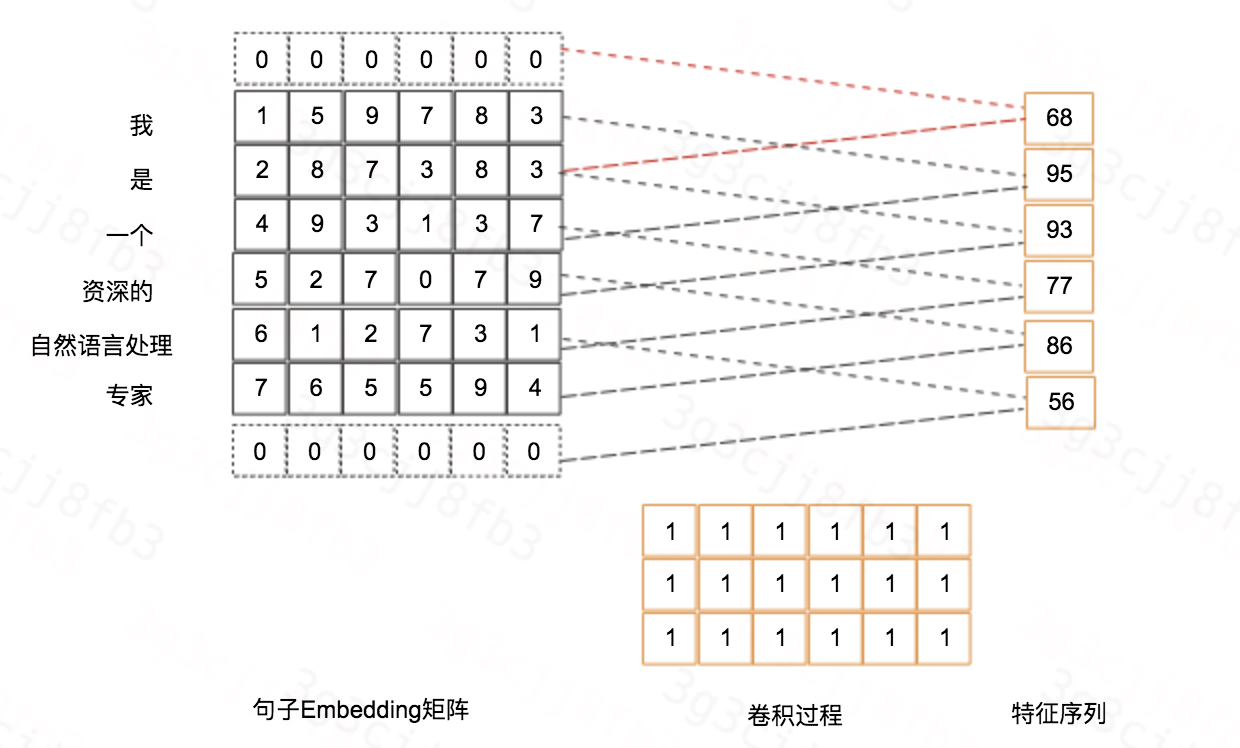
\includegraphics[width=5.5in]{figures/textcnn2.png}
\caption{门控卷积网络的详细结构}
\label{default}
\end{center}
\end{figure}

\begin{table}[h]
	\caption{文本分类评价指标的关键概念}  
	\centering
	\scalebox{0.9}{
		\begin{tabular}{lll}
		  \toprule
		  \midrule
		  错误的正例(FP)& & 被模型错误分为正类的测试集负样本的数量\\
		  \midrule
		  正确的正例(TP)& & 被模型正确分为正类的测试集正样本的数量\\
		  \midrule
		  错误的负例(FN)& & 被模型错误分为负类的测试集正样本的数量\\
		  \midrule
		  正确的负例(TN)& & 被模型正确分为负类的测试集负样本的数量 \\
 		  \bottomrule
		\end{tabular}
	}
\end{table}

我们定义如下的矩阵
$$
M=\left [
\begin{matrix}
\mbox{正确的正例数}(TP) & \mbox{错误的正例数}(FP) \\
\mbox{错误的负例数}(FN) & \mbox{正确的负例数}(TN)
\end{matrix} 
\right ]
$$
我们把这个矩阵称为二分类的混淆矩阵,混淆矩阵的主对角线表示模型正确分类样本的能力,每行的初对角线之外的其他元素表示,模型错分的情况。可以看出模型的精准率定义为第一行主对角元素的值除以整行的和;模型的召回率是第一列主对角元素的值除以整列的和。具体来说
$$
\mbox{精准率}=\frac{\mbox{正确的正例数}(TP)}{\mbox{正确的正例数}(TP) + \mbox{错误的正例数}(FP)} 
$$
$$
\mbox{召回率}=\frac{\mbox{正确的正例数}(TP)}{\mbox{正确的正例数}(TP) + \mbox{错误的负例数}(FN)} 
$$

对于多分类问题,混淆矩阵$M={m_{i,j}|i,j=1,2,\cdots, N}$, 其中$N$表示样本的类别数量,$m_{i,j}$ 表示模型判定样本为第$i$类,但是其实际标签为第$j$类的数量。混淆矩阵反映了模型分类结果和样本实际标注结果的一致程度,显然混淆矩阵的主对角线元素的和表示模型正确分类的样本数量,模型的所有样本的和表示模型的评测样本总量。这里引出多分类问题的第一个指标——准确率acc:
$$
acc = \frac{\sum_{i=1}^{N}m_{i,i}}{\sum_{i=1}^{N}\sum_{j=1}^{N}m_{i,j}} 
$$
多分类问题没有正负样本的概念,但是我们可以定义针对某个类别的精准率和召回率,对于类别$i$其:

$$
i-\mbox{类别的精准率}=\frac{m_{i,i}}{\sum_{j=1}^{N}m_{i,j}} 
$$
$$
i-\mbox{类别的召回率}=\frac{m_{i,i}}{\sum_{j=1}^{N}m_{j,i}} 
$$
这种指标的另一种理解方法是,将第$i$类当成正样本,其他类别当成负样本的二分类精准率和召回率。

\section{经典文本分类技术}
\section{神经网络文本分类技术概述}
传统的文本分类技术主要依托一些经典统计机器学习方法,比如支持向量机、XGBOOST和逻辑回归等技术。这些技术是通用分类技术,可以用于文本分类、图片分类和视频分类等诸多任务,没有针对自然语言信号的单独设计,因此为了能够取得良好的分类效果,工程师必须能够自己做大量的特征工程,例如分词、去除停用词、同义词归一化和文本向量化等诸多繁琐的工作。通常不同的数据集需要不同的特征支持,算法本身只能非常微弱的理解文本语意,因此统计机器学习方法,在神经网络文本分类技术出现之后,由于新的文本分类技术准确率召回率都更好,而且使用更简单;传统的统计机器学习在文本分类领域的应用逐渐变少,甚至有慢慢消失的趋势,因此我们这里不打算做详细的展开。
\subsection{基于CNN的文本分类技术}
在Google 提出word2vec之后,收到深度学习在计算机视觉和语音识别领域的巨大成功,人们便不愿意停留在简单实用统计机器学习进行文本分类,开始有研究这将目光瞄准了卷积神经网络。众所周知2014年的时候,卷积神经网络已经在图像特征提取方面表现出强大的技术能力,图片分类技术也达到令人眼前一亮的程度,特别是在ImageNet数据集上,每年一度的文本分类挑战,\gls{CNN}在逐步展现出非常强大的威力。于是有研究者希望能将\gls{CNN}应用到文本分类领域。这种想法是非常自然的,如图\ref{fig:textcnn1}所示,在计算机看来经过Embedding处理后的句子可以变成了一个矩阵,这和一张单通道的句向量色阶图在计算机看来并无本质上不同。那么我们使用什么样的句子矩阵呢?很容易想到如果一个句子有$N$个词,每个词都使用预训练的词向量来表示,$S=[w_1,w_2,\cdots,w_|S|]$。如果句向量的维度是$H$,我们将句子的词向量序列顺次拼接起来就得到一个$|S| \times H$的矩阵 
$$
M=w_1 \otimes w_2 \otimes \cdots \otimes w_{|S|}
$$
如果把这个矩阵当成一幅单通道的图片,能不能通过图片分类的技术,实现文本分类呢?答案是肯定的,这种技术就是大名鼎鼎的TextCNN。
\begin{figure}[htbp]
\centering
\subfigure[句子向量化后形成的矩阵]{
	\begin{minipage}[t]{0.50\linewidth}
	\centering
	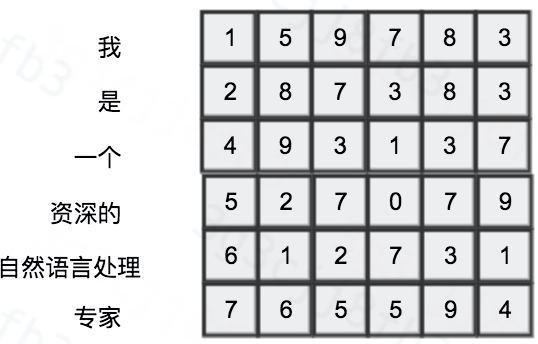
\includegraphics[width=2.5in]{./figures/textcnn1_p1.png}
	%\caption{fig1}
	\end{minipage}%
}
\subfigure[经过色阶处理之后的句子矩阵色阶图]{
	\begin{minipage}[t]{0.50\linewidth}
	\centering
	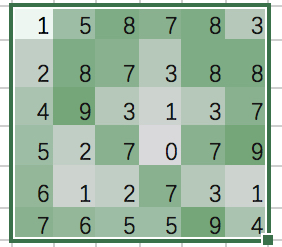
\includegraphics[width=1.8in]{./figures/textcnn1_p2.png}
	%\caption{fig2}
	\end{minipage}%
}%
\caption{句向量矩阵和对应的色阶图}\label{fig:textcnn1}
\end{figure}
\begin{figure}[htbp]
\begin{center}
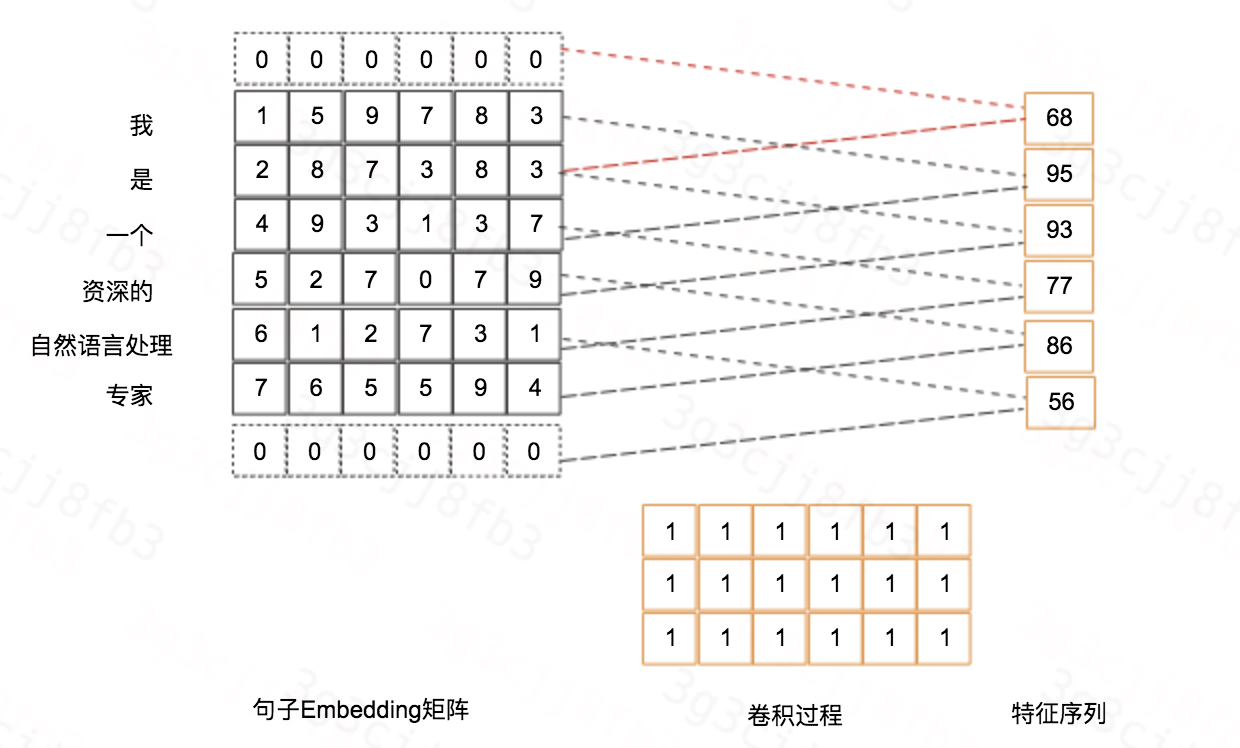
\includegraphics[width=5.8in]{figures/textcnn2.png}
\caption{一个卷积核计算特征的过程}
\label{fig:textcnn2}
\end{center}
\end{figure}

TextCNN的卷积核一般是一个$W$行的矩阵,每行有$H$列($H$一般是奇数),我们定义这个卷积核为$\{K_{i,j}|i=1,2,\cdots,W;j=1,2,\cdots,H\}$。对于这种规格的卷积核通常会在Embeding向量矩阵的前后各加$H/2$列零,这样卷积核从上到下执行一遍就得到了一个$|S| \times 1$的特征序列。如图\ref{fig:textcnn2}所示,卷积核的尺寸为$3 \times 6$。这个例子中,卷积核矩阵内部的值都是$1$,计算结果就相当于窗口元素求和。相当于这个卷积核可以为每个位置取到一个求和特征。一般在TextCNN中同一尺寸的卷积核会有多个,每个卷积核可以捕捉一个位置的词的n-gram特征。特征提取完之后,模型会对同一尺寸卷积核提取的特征序列做挑选,这个挑选过程就是对每个序列特征位置上所有元素求最大。这个求最大的过程被称为max-pooling。假定上述规格的卷积核有$n$个,那么, 就会形成$n$个特征序列,每个特征序列的长度都是$|S|-
W + 1$, 这里可以用一个矩阵来表示,我们记为
$$
M=\{c_{i,j|i=1,2,\cdots, |S|-W+1; j =1,2,\cdots,n}\}
$$
那么经过池化后的特征序列为
$$
C_j=max_{i \in \{1,2,\cdots,|S|-W+1\}}(c_{i,j})
$$
一般会设计几个不同规格的卷积核,每种卷积核生成一个池化特征序列,模型会最终将其拼接在一起后,通过线性投射层后就可以用来计算交叉熵了。有了交叉熵之后就可以训练卷积核,使之提取出有效的特征来。

需要强调两点:第一,模型的最后线性投射层是一个全连接,一般来讲全连接的拟合能力过于强大,会导致模型过拟合,所以可以在这里加一些dropout噪声。第二,句子的Embedding矩阵可以在训练的时候进行进一步训练微调,通常能带来一些指标提升。其实这种预训练外加微调的技术后来被广泛应用到\gls{NLP}领域,发展成为后来的革命性意义的预训练技术。

最后我们给出基于tensorflow框架下的textcnn代码实现 
\begin{lstlisting}[language={python}]
import tensorflow as tf

from model.albert.text_albert import get_shape_list
from model.cnn.text_cnn_config import TextCNNConfig


class TextCNN(object):

  '''
        N -- idcnn_macro_block_num
		B -- batch_size
		S -- seq_len
		E -- emb_size
		F_n -- num_filter
		F_w -- filter_width
		T -- tag_num
  '''

  def __init__(self,
               config: TextCNNConfig,
               is_training,       #train/eval/test
               embedding_matrix,  #embedding 初始化矩阵
               #tag_num,           #类别数量
               input_ids,         #输入id
               segment_ids,       #角色id
               input_mask         #输入id的mask
               ):

    self._config = config
    self._is_training = is_training
    self._embedding_matrix = embedding_matrix

    #self._tag_num = tag_num

    self._input_ids = input_ids
    self._segment_ids = segment_ids
    self._input_mask = input_mask

    self._initializer = tf.contrib.layers.xavier_initializer()

  def get_pooled_output(self, pool_method='max'):

    input_embedding = self.__embedding_layer(input_ids=self._input_ids, segment_ids=self._segment_ids)
    pool_output = self.__cnn_layer_ori(model_inputs=input_embedding)
    return pool_output

  def get_sequence_output(self):

    input_embedding = self.__embedding_layer(input_ids=self._input_ids, segment_ids=self._segment_ids)
    cnn_output = self.__cnn_layer(model_inputs=input_embedding)
    return cnn_output

  def __embedding_layer(self, input_ids, segment_ids):
    '''
    embedding 层
    Input -- B x S
    Output -- B x S x E
    '''
    embedding_matrix_tensor = None
    with tf.name_scope('embedding'):
      # id embedding
      if self._config.embedding_fine_tuning:
        if self._embedding_matrix is not None:
          embedding_matrix_tensor = tf.Variable(initial_value=self._embedding_matrix,
                                                dtype=tf.float32, name="embeddings")
        else:
          embedding_matrix_tensor = tf.get_variable(name="embeddings",
                                                    dtype=tf.float32,
                                                    shape=[self._config.vocab_size, self._config.embedding_size],
                                                    initializer=self._initializer)
      else:
        embedding_matrix_tensor = tf.constant(value=self._embedding_matrix, dtype=tf.float32, name="embeddings")
      # segment embedding
      segment_embedding_matrix_tensor = tf.get_variable(name='role_embedding',
                                                        dtype=tf.float32,
                                                        shape=[self._config.segment_size, self._config.embedding_size],
                                                        initializer=self._initializer)

    with tf.device('/cpu:0'):
      embedding_input = tf.nn.embedding_lookup(params=embedding_matrix_tensor, ids=input_ids)
      segment_input = tf.nn.embedding_lookup(params=segment_embedding_matrix_tensor, ids=segment_ids)
      embedding_input += segment_input
      keep_prob = self._config.embedding_keep_prob if self._is_training else 1.0
      embedding_input = tf.nn.dropout(x=embedding_input, keep_prob=keep_prob)

    return embedding_input

  def __cnn_layer_ori(self, model_inputs):

    # B x S(W) x E(H) -> B x S(W) x E(H) x 1(C)
    model_inputs = tf.expand_dims(input=model_inputs, axis=-1)
    hidden_list = list()

    with tf.variable_scope("cnn_ori"):
      for (i, layer) in enumerate(self._config.layers):
        # 用卷积核提取特征图像
        filter_width = layer
        shape = [filter_width, self._config.embedding_size, 1, self._config.filter_num]
        filter_weights = tf.get_variable(name="idcnn_filter-%d"%i, shape=shape, initializer=self._initializer)
        # B X S x H x Fn  -> B x (S-Fw+1) x 1 x F_n
        layer_input_ = tf.nn.conv2d(input=model_inputs, filter=filter_weights, strides=[1, 1, 1, 1], padding="VALID",
                                    name="init_layer")
        # 执行特征图的池化
        b,w,h,fn = get_shape_list(tensor=layer_input_, expected_rank=4)
        pool_output = tf.nn.max_pool(value=layer_input_, ksize=[1, w, 1, 1], strides=[1, 1, 1, 1], padding='VALID')
        pool_output = tf.reshape(tensor=pool_output, shape=[b, fn])
        hidden_list.append(pool_output)

    cnn_output = tf.concat(values=hidden_list, axis=-1)

    return cnn_output

  def __cnn_layer(self, model_inputs):

    '''
    idcnn/cnn layer
    Input -- B x S x E
    Output -- B*S x F_n*N
    '''
    # B x S x E -> B x 1 x S x E
    model_inputs = tf.expand_dims(input=model_inputs, axis=1)

    with tf.variable_scope("idcnn"):
      # 1. init layer
      shape = [1, self._config.filter_width, self._config.embedding_size, self._config.filter_num]
      filter_weights = tf.get_variable(name="idcnn_filter", shape=shape, initializer=self._initializer)
      # B x 1 X S x E -> B x 1 x S x F_n
      layer_input_ = tf.nn.conv2d(input=model_inputs, filter=filter_weights,
                                  strides=[1, 1, 1, 1], padding="SAME", name="init_layer")

      # 2. dilated cnn layers
      final_output = list()
      total_width = 0
      for c_t in range(self._config.idcnn_macro_block_num):
        layer_input = layer_input_
        for layer_index in range(len(self._config.layers)):
          layer = self._config.layers[layer_index]
          dilation = int(layer)
          with tf.variable_scope("atrous_conv_l-%d" % layer_index, reuse=tf.AUTO_REUSE):
            w = tf.get_variable(name="w",
                                shape=[1, self._config.filter_width, self._config.filter_num, self._config.filter_num],
                                initializer=self._initializer)
            b = tf.get_variable(name="b", shape=[self._config.filter_num])
          if not self._config.use_dilated:
            dilation = 1
          layer_y = tf.nn.atrous_conv2d(value=layer_input, filters=w, rate=dilation, padding="SAME")
          layer_y = tf.nn.bias_add(value=layer_y, bias=b)

          layer_y = tf.nn.relu(layer_y)
          if layer_index == len(self._config.layers) - 1:
            final_output.append(layer_y)
            total_width += self._config.filter_num
          layer_input = layer_y

      y = tf.concat(values=final_output, axis=3)
      keep_prob = self._config.idcnn_keep_prob if self._is_training else 1.0
      y = tf.nn.dropout(x=y, keep_prob=keep_prob)
      # B x 1 x S x F_n*N -> B x S x F_n*N
      y = tf.squeeze(input=y, axis=[1])
      return y
      
\end{lstlisting}
针对上述实现需要注意的是,如果要使用$L2$正则,请不要直接使用常见的优化器Adam而要使用其优化版本——AdamW。如果作为序列标注任务的特征提取模块,卷积的使用方式于文本分类略有不同,因为需要保证卷积后特征序列的长度和原始句子的长度相等,因此需要做一些前后补零工作。具体的来说就对原始的文本的前后各补$W/2$的$0$,以保证经过卷积后,输出的尺寸和原始文本输入的形状相同。我们在上面的代码示例中,也提供了这个的实现。

\subsection{基于RNN的文本分类技术}
我们从TextCNN 中可以清楚的看出,模型在尝试捕捉文本的n-gram特征,并没有很好的建模文本的序列时序特征,于是很多算法工程师,尝试使用\gls{RNN}/\gls{GRU}/\gls{LSTM} 去建模句子数学表示,然后将句子的数学表示,透过一个全连接网络,通过softmax构建分类损失。这种想法非常简单,但是在实践中人们观察到非常好的效果,至少在新闻文本分类数据上,基于\gls{LSTM}的模型效果,并不比TextCNN差。
通常可以用\gls{RNN}单元的最后一个时刻的\gls{LSTM}/\gls{GRU}单元输出作为句子的数学表示,也可以把所有时刻的输出拼接起来作为句子的数学表示,然后构造分类损失,从实验看起来,两种表示句子语意的方法做出来的分类器并无太大的性能差异。另外一个Trick,大家可以试试,就是先把句子序列倒置一下,然后再通过循环神经网络,通常会比正序效果要好一点。模型的结构参见图\ref{fig:textrnn1}。
\begin{figure}[htbp]
\begin{center}
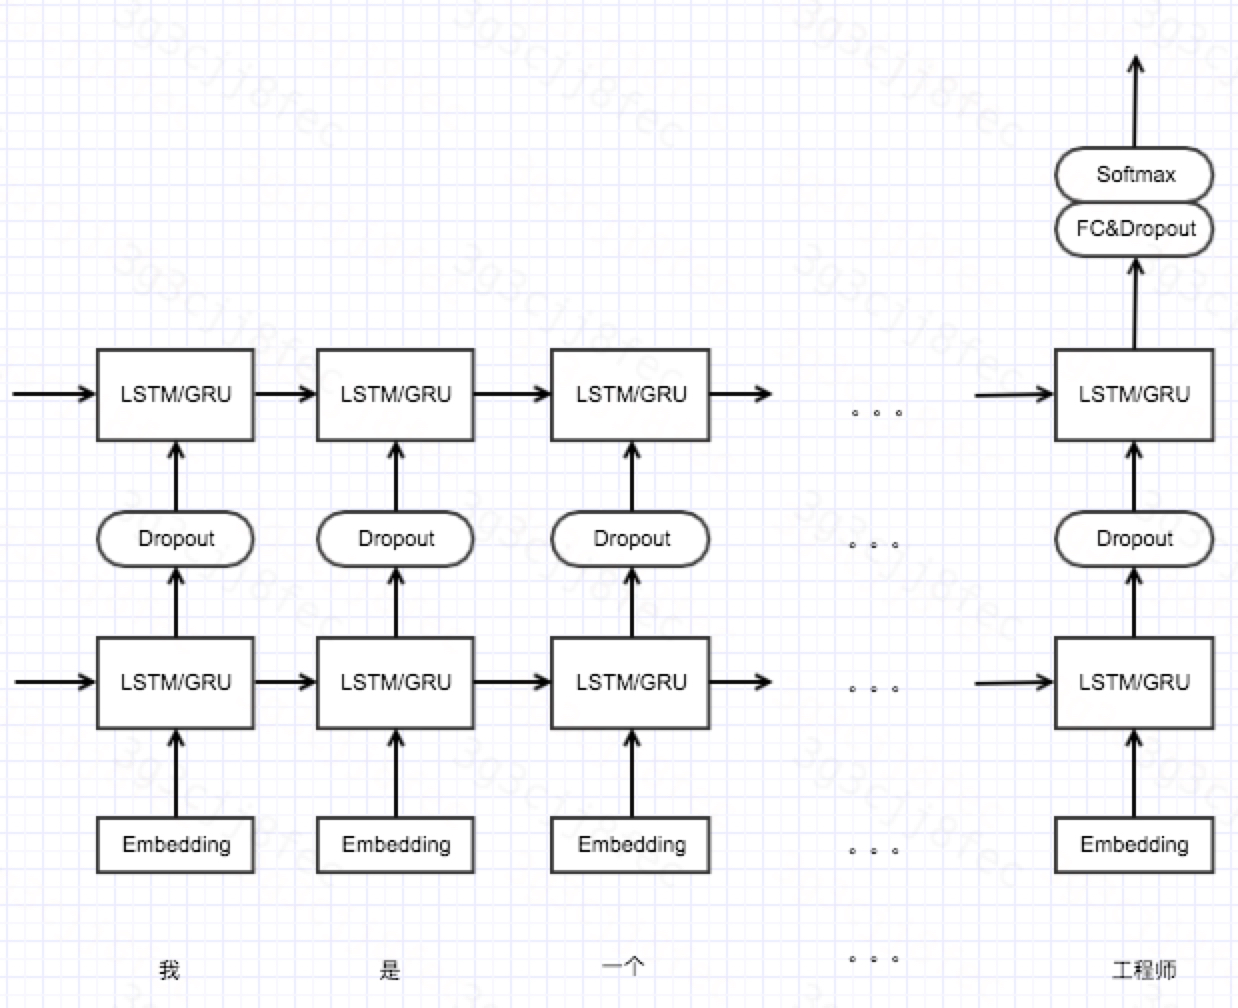
\includegraphics[width=5.6in]{figures/textrnn1.png}
\caption{TextRNN 的网络结构}\label{fig:textrnn1}
\end{center}
\end{figure}

最后我们给出一个参考实现
\begin{lstlisting}[language={python}]
class RnnModel(object):
	def __init__(self, config):
		self.config = config

	def create_model(self):
		pm = self.config
		self.input_x = tf.placeholder(tf.int32, shape=[None, pm.seq_length], name='input_x')
		self.input_y = tf.placeholder(tf.float32, shape=[None, pm.num_classes], name='input_y')
		self.seq_length = tf.placeholder(tf.int32, shape=[None], name='sequen_length')
		self.keep_prob = tf.placeholder(tf.float32, name='keep_prob')
		embedding = tf.get_variable('embedding', shape=[pm.vocab_size, pm.embedding_dim],
																initializer=tf.constant_initializer(pm.pre_trianing))
		self.embedding_input = tf.nn.embedding_lookup(embedding, self.input_x)
		cells = [tf.nn.rnn_cell.DropoutWrapper(tf.nn.rnn_cell.LSTMCell(num_units=pm.hidden_dim,name='cell-'+str(i)),
																					 output_keep_prob=self.keep_prob)
						 for i in range(pm.num_layers)]
		cell = tf.nn.rnn_cell.MultiRNNCell(cells, state_is_tuple=True)
		output, _ = tf.nn.dynamic_rnn(cell=cell, inputs=self.embedding_input, sequence_length=self.seq_length,
																	dtype=tf.float32)
		output = output[:, -1, :]
		logits = tf.layers.dense(inputs=output, units=pm.num_classes)
		logits = self.out_drop = tf.nn.dropout(logits, keep_prob=self.keep_prob)
		predict = tf.argmax(tf.nn.softmax(logits), 1, name='predict')
		losses = tf.nn.softmax_cross_entropy_with_logits_v2(logits=logits, labels=self.input_y)
		loss = tf.reduce_mean(losses)
		return predict, loss
	
\end{lstlisting}

\subsection{基于RNN和CNN结合的文本分类技术}
我们知道TextCNN只使用了单层的若干不同窗口尺寸\gls{CNN}进行特征捕捉,因此我们可以看到他忽视了序列信息的建模,而且窗口尺寸的选择需要网格搜索,因此比较复杂。而\gls{RNN}虽然能够捕捉序列信息特征,但是它明显是有偏的,因为\gls{LSTM}会遗忘距离句尾过远的句首词,但是对于文本分类,所有的词汇的语意信息都是同等重要的。如何能够很好的利用\gls{RNN}捕捉语意特征,有能够使之无偏差呢?人们想到了结合\gls{RNN}和\gls{CNN}来进行文本分类,也就是TextRCNN网络。这个网络使用双向\gls{LSTM}/\gls{GRU}来建模句子中的每个词和其上下文环境。所谓双向\gls{LSTM}/\gls{GRU} 就是,从左到右执行一次,然后从右到左执行一次,然后将输出结果拼接在一起。

RCNN网络模型分两层——词汇表示层和句子特征表示层。
\begin{figure}[htbp]
\begin{center}
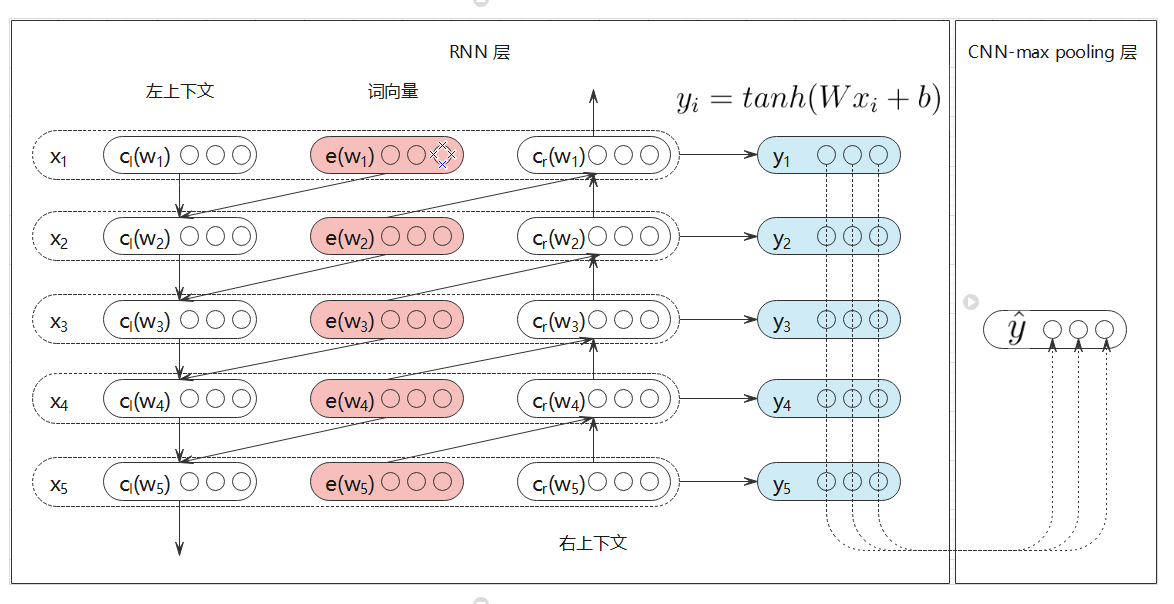
\includegraphics[width=5.6in]{figures/textrcnn1.png}
\caption{TextRCNN 的网络结构}
\label{fig:textrcnn1}
\end{center}
\end{figure}
\subsubsection{RNN-词汇表示层}
词汇表示层的设计是基于双向\gls{RNN}模型,其输出是词汇的隐语意表示$y_i$,其中词汇$w_i$的表示$x_i$由三部分拼接组成: 词汇左上下文$c_l(w_i)$、词汇自身的embedding$e(w_i)$和词汇的右上下文$c_r(w_i)$:
$$
x_i=[c_l(w_i);e(w_i);c_r(w_i)]
$$
之后模型通过一个全连接层后得到隐语意表示向量:
$$
y_i=tanh(Wx_i+b)
$$
\subsubsection{CNN Pooling-句子特征表示层}
句子表示层本质上是一个max-pooling操作,max-pooling 操作是逐元素计算的,相当于从所有元词的隐语意表示向量的每一个元素位置挑出最大的组成一个向量。
$$
\hat{y} = max_{i=1}^{n}y_i 
$$
其中$n$表示句子的长度。

\gls{CNN} Pooling操作有助于模型从整个句子中挑选出对分类结果有帮助的特征,因此克服了TextCNN 窗口视野太小和无法建模序列特征的缺点,同时克服了TextRNN 遗忘句首元素的有偏性。研究表明TextRCNN 相对TextCNN/TextRNN有一到两个百分点的准确度提升。

最后,我们给出一个基于tensorflow 的代码实现:

\begin{lstlisting}[language={python}]
class TextRCNN:
	def __init__(self, config):

		self.input_text = tf.placeholder(tf.int32, shape=[None, sequence_length], name='input_text')
		self.input_y = tf.placeholder(tf.float32, shape=[None, num_classes], name='input_y')
		self.dropout_keep_prob = tf.placeholder(tf.float32, name='dropout_keep_prob')
		self.config = config

	def create_model(self):
		text_length = self.config.text_length

		W_text = tf.Variable(tf.random_uniform([self.config.vocab_size, self.config.word_embedding_size], -1.0, 1.0),
															name="W_text")
		embedded_chars = tf.nn.embedding_lookup(W_text, self.input_text)
		fw_cell = tf.nn.rnn_cell.BasicLSTMCell(self.config.hidden_size)
		fw_cell = tf.nn.rnn_cell.DropoutWrapper(fw_cell, output_keep_prob=self.dropout_keep_prob)
		bw_cell = tf.nn.rnn_cell.BasicLSTMCell(self.config.hidden_size)
		bw_cell = tf.nn.rnn_cell.DropoutWrapper(bw_cell, output_keep_prob=self.dropout_keep_prob)
		(output_fw, output_bw), states = tf.nn.bidirectional_dynamic_rnn(cell_fw=fw_cell, cell_bw=bw_cell,
																			inputs=embedded_chars, sequence_length=text_length, dtype=tf.float32)
		shape = [tf.shape(output_fw)[0], 1, tf.shape(output_fw)[2]]
		c_left = tf.concat([tf.zeros(shape), output_fw[:, :-1]], axis=1, name="context_left")
		c_right = tf.concat([output_bw[:, 1:], tf.zeros(shape)], axis=1, name="context_right")

		x = tf.concat([c_left, embedded_chars, c_right], axis=2, name="x")
		embedding_size = 2 * context_embedding_size + word_embedding_size

		W2 = tf.Variable(tf.random_uniform([self.config.embedding_size, self.config.hidden_size], -1.0, 1.0), name="W2")
		b2 = tf.Variable(tf.constant(0.1, shape=[self.config.hidden_size]), name="b2")
		y2 = tf.tanh(tf.einsum('aij,jk->aik', x, W2) + b2)
		y3 = tf.reduce_max(y2, axis=1)

		W4 = tf.get_variable("W4", shape=[self.config.hidden_size, self.confignum_classes], 
												 initializer=tf.contrib.layers.xavier_initializer())
		b4 = tf.Variable(tf.constant(0.1, shape=[self.config.num_classes]), name="b4")
		logits = tf.nn.xw_plus_b(y3, W4, b4, name="logits")
		predictions = tf.argmax(logits, 1, name="predictions")

		# Calculate mean cross-entropy loss
		losses = tf.nn.softmax_cross_entropy_with_logits(logits=logits, labels=self.input_y)
		loss = tf.reduce_mean(losses)
		return predictions, loss
\end{lstlisting}

\subsection{神经网络快速文本分类技术-FastText}
\begin{figure}[H]
	\begin{center}
		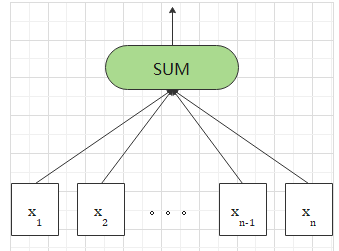
\includegraphics[width=4.0in]{figures/fasttext1.png}
		\caption{FastText 的网络结构}
		\label{fig:fasttext}
	\end{center}
\end{figure}
随着计算机技术的快速发展,大规模文本分类技术进入了人们的应用视野,但是面对超大规模的数据集和超大规模的标签数量,基于深度神经网络复杂结构的文本分类算法的训练和推理速度都难以满足需求。事实上,复杂神经网络的计算量主要来自两个方面,一方面是模型本身特征抽取阶段,需要大量的运算,有些网络甚至无法并行化(如\gls{RNN});另一方面是在softmax层由于标签数量巨大,简单的softmax 运算就非常耗时。为了能够应对具有超大标签种类的大规模数据集训练和推理需求,人们采取了两个精简策略:第一,精简特征抽象网络;第二,优化softmax。我们知道词向量的训练就具有训练集巨大且标签种类巨大的特点,因此人们已经积累了足够的技术能力,来解决目前的问题。我们在词向量训练那一章提到过,加速词向量训练有两种方法来减低softmax层的开销:一种是使用采样的方法,逼近softmax运算;另一种是使用层次化softmax来模拟softmax运算。Fast采用了后者,具体的理论和实现,
我们就不赘述了。FastText的模型结构如下所示,其实和\gls{CBOW}的结构非常相似,只不过它把整个句子当成了窗口,另外因为不需要预测中心词,所以没有在窗口中心做任何的挖空处理。其结构如图\ref{fig:fasttext}所示,输入层的词向量,经过求平均之后直接执行分层softmax就可以构建分类损失了。由于结构上的精简,FastText 的训练速度和推理速度可以做到神经网络文本分类模型的数百倍甚至更快。

我们知道FastText并没有考虑句子中不同的词汇之间的语意序列关系,因此文章使用N-gram 特征, 相当于建模了句子的偏序关系。但是这带来的问题,是词表会急速膨胀,违背了N-gram 设计的初衷,因此在工业领域很少使用。举个例子来说明一下,假定输入的句子是$n$个词$w_1,w_2,\cdots,w_n$,那么所有的bi-gram有$[w_1,w_2],[w_2,w_3],\cdots,[w_{n-1},w_n]$ 个,这个数量是非常惊人的。

最后我们给出一个基于softmax的FastText的实现:
\begin{lstlisting}[language={Python}]
class FastText():
	def __init__(self, seq_length, num_classes, vocab_size):
		self.seq_length = seq_length
		self.num_classes = num_classes
		self.vocab_size = vocab_size
		self.embedding_dim = 128

		self.input_x = tf.placeholder(tf.int32, [None, self.seq_length], name='input_x')
		self.input_y = tf.placeholder(tf.float32, [None, self.num_classes], name='input_y')
		self.learning_rate = tf.placeholder(tf.float32, name='learn_rate')

	def create_model(self):
		embedding = tf.get_variable("embedding", [self.vocab_size, self.embedding_dim])
		embedding_inputs = tf.nn.embedding_lookup(embedding, self.input_x)
		mean_sentence = tf.reduce_mean(embedding_inputs, axis=1)
		self.logits = tf.layers.dense(mean_sentence, self.num_classes,
																	kernel_regularizer=tf.contrib.layers.l2_regularizer(0.001),
																	name='fc2')
		self.y_pred_cls = tf.argmax(tf.nn.softmax(self.logits), 1, name="pred")

		cross_entropy = tf.nn.softmax_cross_entropy_with_logits(
			logits=self.logits, labels=self.input_y)
		self.loss = tf.reduce_mean(cross_entropy, name="loss")

\end{lstlisting}

\subsection{长文本分类—HAN}
对于长文本,无论是TextCNN 还是TextRNN都没有充分利用文本的结构信息。长文本通常会分为若干短句子,短句子之间通过标点符号来分割,每个短句子都是一个相对独立的语意单元。\gls{HAN}网络尝试通过分层语意表示的方法来构建篇章级别的文本表示,这种做法利用了长文本的基本结构,能在词汇级别和句子级别分别建立注意力模型,从而使得分类损失能够和关键的词汇和句子表示建立联系,使得该算法在长文本分类领域成为具有代表性地工作之一。

模型的整体结构如图\ref{fig:han1}所示,分为三个主要的层次——词编码和自注意力层、句编码和自注意力层以及分类层。

\begin{figure}[H]
\begin{center}
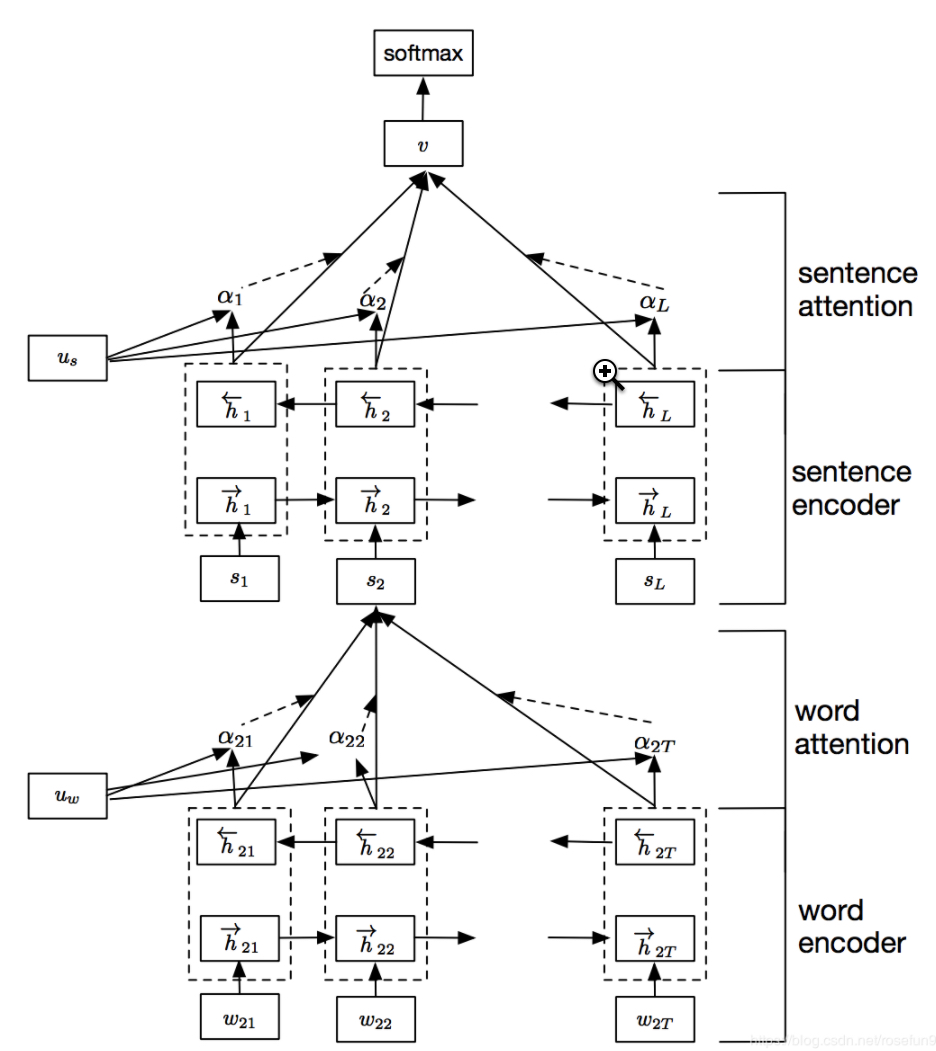
\includegraphics[width=5.6in]{figures/han1.png}
\caption{HAN 的网络结构}\label{fig:han1}
\end{center}
\end{figure}

\subsubsection{词编码表示}

假定一个段落包含$L$个句子每个句子包含$T_i$个词语, 我们用$w_{i,t}$表示第$i$个句子的第$t$个词汇的one-hot表示。模型首先通过左乘一个Embedding矩阵$W_e$得到段落中每个词的向量表示:
$$
x_{i,t} = W_ew_{i,t}
$$
这个词向量序列会通过一个双向的\gls{GRU}网络得到每个位置的词语意表示$h_{i,t}=[\overrightarrow{h_{i,t}};\overleftarrow{h_{i,t}}]$, 其中
$$
\begin{aligned}
\overrightarrow{h_{i,t}} &= \overrightarrow{GRU}(x_{i,t}),t\in [1,T_i]\\
\overleftarrow{h_{i,t}} &=\overleftarrow{GRU}(x_{i,t}),t\in [1,T_i]
\end{aligned}
$$
有了词的编码表示,我们计算这些词的编码之间的自注意力模型,进一步建立词汇的语意联系
$$
\begin{aligned}
u_{i,t} &= tanh(W_{w}h_{i,t} + b_w)\\
\alpha_{i,t} &= \frac{
	exp(u_{i,t}^\top u_w)
}{\sum_{t}exp(u_{i,t}^\top u_w)}\\
s_i &= \sum_{t}(a_{i,t}h_{i,t})  
\end{aligned}
$$
其中$u_w$ 可以被视为对句子关键语意的挑选学习,这个变量的随机初始化的,并且是可学习的一个训练变量,希望模型在学习的过程中能够通过$u_w$作为注意力的Query,习得特征挑选的方法。

\subsubsection{句编码表示}
模型的句编码表示的输入是词编码表示序列$s_i$,词编码序列会首先通过一个双向\gls{GRU}网络得到每个句子的句编码表示$h_i=[\overrightarrow{h_{i}};\overleftarrow{h_{i}}]$,其中
$$
\begin{aligned}
\overrightarrow{h_{i}} &= \overrightarrow{GRU}(s_i),i\in [1,L]\\
\overleftarrow{h_{i}} &=\overleftarrow{GRU}(s_i),i\in [1,L]
\end{aligned}
$$
和词编码表示类似,我们通过自注意力模型,进一步建立句子的语意联系
$$
\begin{aligned}
u_{i} &= tanh(W_sh_{i} + b_s)\\
\alpha_{i} &= \frac{
	exp(u_{i}^\top u_s)
}{\sum_{t}exp(u_{i}^\top u_s)}\\
v &= \sum_{t}(a_{i}h_{i})  
\end{aligned}
$$
其中,$u_s$可以被视为段落语意的一个高维的表示,用于正则化注意力的归一化系数,这个变量的随机初始化的,并且是可学习的一个训练变量,类似于记忆网络。最后$v$通过线性投射层后,就可以构造损失函数了。

最后我们给出\gls{HAN}的一个代码实现:
\begin{lstlisting}[language={Python}]
class TextHAN:

	def __init__(self, config):
		self._config = config

	def __embedding_layer(self, input_ids, segment_ids):

		embedding_matrix_tensor = None
		with tf.name_scope('embedding'):
			# id embedding
			if self._config.embedding_fine_tuning:
				if self._embedding_matrix is not None:
					embedding_matrix_tensor = tf.Variable(initial_value=self._embedding_matrix,
																								dtype=tf.float32, name="embeddings")
				else:
					embedding_matrix_tensor = tf.get_variable(name="embeddings",
																										dtype=tf.float32,
																										shape=[self._config.vocab_size, self._config.embedding_size],
																										initializer=self._initializer)
			else:
				embedding_matrix_tensor = tf.constant(value=self._embedding_matrix, dtype=tf.float32, name="embeddings")
			embedding_input = tf.nn.embedding_lookup(params=embedding_matrix_tensor, ids=input_ids)
			# segment embedding
			segment_embedding_matrix_tensor = tf.get_variable(name='role_embedding',
																												dtype=tf.float32,
																												shape=[self._config.segment_size, self._config.embedding_size],
																												initializer=self._initializer)
			segment_input = tf.nn.embedding_lookup(params=segment_embedding_matrix_tensor, ids=segment_ids)

		embedding_input += segment_input
		keep_prob = self._config.embedding_keep_prob if self._is_training else 1.0
		embedding_input = tf.nn.dropout(x=embedding_input, keep_prob=keep_prob)

		return embedding_input

	def __bi_rnn_layer(self, model_inputs, sequence_length, cell=tf.nn.rnn_cell.BasicLSTMCell, scope_name="none"):

		keep_prob = self._config.cell_keep_prob if self._is_training else 1.0

		fw_cell = cell(num_units=self._config.hidden_size, name="fw-" + scope_name)
		fw_cell = tf.nn.rnn_cell.DropoutWrapper(fw_cell, output_keep_prob=keep_prob)
		bw_cell = cell(num_units=self._config.hidden_size, name="bw-" + scope_name)
		bw_cell = tf.nn.rnn_cell.DropoutWrapper(bw_cell, output_keep_prob=keep_prob)
		outputs, output_states = tf.nn.bidirectional_dynamic_rnn(cell_fw=fw_cell,
																														 cell_bw=bw_cell,
																														 dtype=tf.float32,
																														 inputs=model_inputs,
																														 sequence_length=sequence_length)

		return outputs, output_states

	def __attention_layer(self, model_inputs, hidden_size, scope_name="none"):

		# b x s x 2h
		attention_context_vector = tf.get_variable(name=scope_name + "context",
																							 shape=[hidden_size * 2],
																							 dtype=tf.float32)
		input_projection = tf.layers.dense(inputs=model_inputs, units=hidden_size * 2, activation=tf.tanh)

		# b x s x 2h -> b x s x 1
		vector_attn = tf.reduce_sum(tf.multiply(input_projection, attention_context_vector), axis=2, keep_dims=True)
		attention_weights = tf.nn.softmax(vector_attn, dim=1)  # b x s x 1
		# b x s x 2h
		weighted_projection = tf.multiply(model_inputs, attention_weights)
		# b x 2h
		outputs = tf.reduce_sum(weighted_projection, axis=1)

		return outputs

	def __sent_encode(self, sent_inputs, sent_masks, max_sent_in_doc, max_word_in_sent):

		# B x Ns x Nw x H -> B*Ns x Nw x H
		sent_inputs = tf.reshape(tensor=sent_inputs, shape=[-1, max_word_in_sent, self._config.hidden_size])
		# B x Ns x Nw  -> B*Ns x Nw
		sent_masks = tf.reshape(tensor=sent_masks, shape=[-1, max_word_in_sent])

		sequence_length = tf.reduce_sum(input_tensor=sent_masks, axis=-1)
		# B*Ns x Nw x H -> B*Ns x Nw x 2H
		rnn_outputs, _ = self.__bi_rnn_layer(model_inputs=sent_inputs, sequence_length=sequence_length, scope_name='sent')
		# B*Ns x 2H
		attention_outputs = self.__attention_layer(model_inputs=rnn_outputs, hidden_size=self._config.hidden_size, scope_name='sent')

		# B x Ns x 2H
		outputs = tf.reshape(tensor=attention_outputs,
												 shape=[-1, max_sent_in_doc, self._config.hidden_size*2])
		# B x Ns
		output_masks = tf.reshape(tensor=tf.sign(x=tf.abs(x=tf.reduce_sum(input_tensor=sent_masks, axis=-1))),
															shape=[-1, max_sent_in_doc])
		return outputs, output_masks

	def __doc_encode(self, doc_inputs, doc_masks):
		# B x Ns -> B
		sequence_length = tf.reduce_sum(input_tensor=doc_masks, axis=-1)
		# B x Ns x 2H -> B x Ns x 4H
		rnn_outputs, _ = self.__bi_rnn_layer(model_inputs=doc_inputs, sequence_length=sequence_length, scope_name="doc")
		outputs = self.__attention_layer(model_inputs=rnn_outputs, hidden_size=2*self._config.hidden_size, scope_name="doc")
		return outputs

	def create_model(self, inputs, input_masks):
		outputs, output_masks = self.__sent_encode(sent_inputs=inputs, sent_masks=input_masks,
											 													max_word_in_sent=self._config.max_word_in_sent,
											 													max_sent_in_doc=self._config.max_sent_in_doc)
		outputs = self.__doc_encode(doc_inputs=outputs, doc_masks=output_masks)
		return outputs
\end{lstlisting}


除了\gls{HAN} 之外,长文本分类领域还有一类基于门控循环网咯或者门控卷积网络的分层建模方法,简单来讲就是用CNN或者RNN进行词编码,然后在句子级别使用门控网络建模句子语意。但是从实验效果上看,他们的效果明显比\gls{HAN}要弱一些,这里就不详细展开了,有兴趣的读者可以自行阅读相关的论文。

\subsection{亚词汇级别文本分类-charCNN}
在文本分类领域,有这样一种场景,其文本表意非常杂乱,比如是一个\gls{ASR} 模块识别出来的,由于在实际生活中,很多人发音并不标准,带有很明显的地域发音特点, 相当于引入了很多错误的知识。特别是在中文环境,存在大量的方言区,我们不可能为每个方言区训练一套子语言模型,因此\gls{ASR}识别之后的文本句法不通顺现象更加严重,为此,人们希望从发音的角度进行文本识别。将文本表音的音素代替汉字作为基本单元,通过精心设计的卷积神经网络,能起到抑制方言噪声的作用。这项研究最初是基于英文字符的,是用字符代替单词作为基本文本单元,通过卷积神经网络进行文本分类。

Xiang Zhang等人提出的模型结构包含6个卷积层和6个全连接层,每个卷积层后面会跟1个池化层。为了说明卷积和池化的过程,我们举一个简单的例子,这个例子仅仅是为了说明卷积和池化的过程,在图\ref{fig:charcnn1}这个例子中,有一段文本经过符号化后,我们对每个符号进行$4$维度Embedding变成一个$4 \times 8$的矩阵,这个矩阵经过$4$个宽度为$3$的卷积核经过一维卷积之后,形成一个$(8-3+1) \times 4$的特征图像,随后经过一个宽度为$3$步长为$3$的池化之后,得到一个$(6/3)\times 4$的池化特征图,并进入下一层。每个全连接层后面都会接一个dropout层。为了说明网络的完整结构我们举一个完整的网络例子,这个例子的每个句子的长度是1014,最后形成一个长为34的向量序列。
\begin{figure}[h]
	\begin{center}
	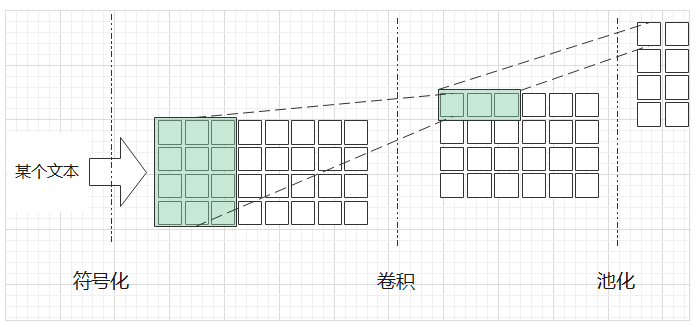
\includegraphics[width=5.6in]{figures/charcnn1.png}
	\caption{charCNN的卷积结构示例}
	\label{fig:charcnn1}
\end{center}
\end{figure}

\begin{table}[h]
	\caption{charCNN的卷积网络结构}  
	\label{tab:schedule}
	\centering
	\scalebox{0.9}{
		\begin{tabular}{l|cccccc}
			\hline
			前提  	& 第1层 & 第2层& 第3层& 第4层& 第5层& 第6层\\
			\hline
			卷积宽度  			  & 7 & 7 & 3 &3 &3 &3 \\
			卷积后的结果  		& 1008&330& 108&106&104&102\\
			池化宽度和步长 	   &3,3 &3,3&-&-&-&3,3\\
			池化后的结果 			&336 &110&-&-&-&34 \\
			\hline
		\end{tabular}	
	}
\end{table}

最后我们给出基于上述例子的char\gls{CNN} 的代码实现:

\begin{lstlisting}
	class CharCNN(_Classifier):

    def _get_embeddings(self, features, mode=tf.estimator.ModeKeys.TRAIN):
        
        embedding = Embedding(self._params['embedding_specs'])
        embedding.build(None)
        return embedding.call(features)          
            
        
    def _encode(self, embeddings, lengths=None, mode=tf.estimator.ModeKeys.TRAIN):

        conv_layers = self._params.get('conv_layers', None)
        
        if conv_layers is None:
            conv_layers = [
                [256, 7, 3],
                [256, 7, 3],
                [256, 3, None],
                [256, 3, None],
                [256, 3, None],
                [256, 3, 3]
                ]

        x = embeddings

        vec_dim = self._params.get('seq_len', 1014)

        for i, cl in enumerate(conv_layers):
            
            vec_dim -= (cl[1] - 1)

            x = tf.layers.conv1d(x, cl[0], cl[1], activation=tf.nn.relu, name='Conv_%d' % i)
            if not cl[2] is None:
                
                vec_dim -= cl[2]
                vec_dim //= cl[2]
                vec_dim += 1
                
                x =  tf.layers.max_pooling1d(x, cl[2], cl[2], name='Pool_%d' % i)
        
        vec_dim *= cl[0]
        
        x = tf.reshape(x, [-1, vec_dim])

        return x
\end{lstlisting}

\section{句对分类技术}
在文本分类领域,有一些和句子对有关的任务,其中最有影响力的是自然语言推理。自然语言推理的任务是识别给定的两个句子的语意关系是不是无关、蕴含和矛盾。所谓无关和矛盾是容易理解的,所谓蕴含是指,其中一个文本作为前提(premise),另一个文本作为假设(hypothesis),如果根据前提P能够推理得出假设H,那么就说P蕴含H,记做P$\rightarrow$ H。这跟一阶逻辑中的蕴含关系是类似的。我们举个例子,如果我们看到“一只狗在雪地里玩足球”,那么如果别人跟我们讲“一个哺乳动物在雪地里玩足球”,我们认为事实是成立的。这种关系就叫蕴含,因为狗属于哺乳动物因此可以根据前提推断出假设。
\begin{table}[h]
	\caption{自然语言推理任务的句对关系}  
	\label{tab:schedule}
	\centering
	\scalebox{0.9}{
		\begin{tabular}{llll}
		  \toprule
		  \midrule 
		  前提  	& 		& 一只狗在雪地里玩足球 & 关系\\
		  \midrule
		  假设  	& 例子1 & 一个哺乳动物在雪地里玩足球 & 蕴含\\
		  	   	& 例子2 & 一个猫在雪地里玩足球 		& 矛盾\\
		  	   	& 例子3 & 一只宠物正在和他的主人玩 	& 中立\\
		  \bottomrule
		\end{tabular}
	}
\end{table}

目前的句对分类算法包含两个主要的挑战,第一个是构建句子的语意表示;第二个是建模句子之间的语意关系。目前学术界对句子语意建模的方法主要有两种:一种是基于双向\gls{LSTM}/\gls{GRU}的,具有代表意义的网络包括InferSent和ESIM,一种是基于卷积神经网络的,代表网络有ABCNN。句子之间语意关系的建模,目前有三种,第一种是InferSent为代表的简单计算拼接;第二种是基于交互Attention的代表有ABCNN;第三种是基于卷积网络的,代表网络是PWIM网络,这种方式从效果上看比较一般,而且实现起来比较繁琐,我们这里就不详细介绍了。我们下面来挑选几个具有代表性地网络来介绍。

\subsection{InferSent}
InferSent 网络最初提出的时候,并不是用来解决自然语言推理(\gls{NLI})问题的,只是利用SNLI数据集来训练句子的向量表示。网络的结构也比较简单,如图\ref{fig:infersent1}所示。首先将数据的前提句$P=[p_1,p_2\cdots,p_n]$和假设句$H=[h_1,h_2\cdots,h_n]$分别用两个双向\gls{LSTM}/\gls{CNN}或者\gls{SAN}编码之后得到其向量化的表示——$U=[u_1,u_2,\cdots,u_n]$和$V=[v_1,v_2,\cdots,v_n]$,经过简单的数学运算后拼接在一起得到特征的隐层表示$[U;V;|U \ominus V|;U\otimes V]$,通过全连接网络作为\gls{MLP}层的输入。
\begin{figure}[h]
\begin{center}
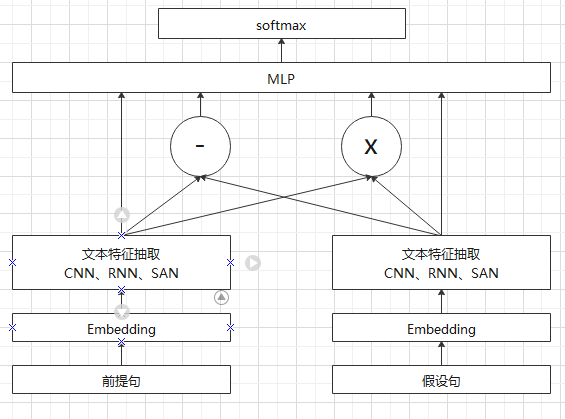
\includegraphics[width=5.6in]{figures/infer_sent.png}
\caption{InferSent网络结构}
\label{fig:infer_sent}
\end{center}
\end{figure}
\subsection{ABCNN}
ABCNN 是基于\gls{CNN}和注意力结合的算法,作者基于\gls{CNN}双塔孪生结构进行注意力改造提出了三种改造方法:$ABCNN-1$,卷积前注意力方案;$ABCNN-2$,卷积后注意力加权方案;$ABCNN-3$,卷积前注意力和卷积后注意力加权结合方案。

在我们介绍每个网络的特点之前,需要先介绍一下本文使用的Attention 方案,假定存在两个句子的向量表示$P=[p_1,p2,\cdots,p_n]$和$H=[h_1,h2,\cdots,h_n]$,那么他们的互相注意力矩阵$A=\{a_{i,j}|i,j=1,2,\cdots,n\}$按照如下方式计算:
$$
a_{i,j} = \frac{1}{1+\|p_i-h_j\|}
$$
当然,这是一种注意力计算方法,还有其他的方法,当前的注意力方案强调的两个向量的欧几里得距离,我们可以看到当两个句子对应的词越小那么这个值就越大,$A[i,:]$可以认为$P$句子的第$i$个词向量到$H$句子的词向量的句子的语意距离分布。
\subsubsection{卷积前注意力方案}
这种方法在每层卷积执行前,会对输入层做一次注意力矩阵计算,之后注意力矩阵会左乘一个形变矩阵。得到一个和卷积的输入层尺寸相同的矩阵,我们称之为卷积交互通道矩阵,
$$
\begin{aligned}
\overline{H} = W_0A^{T}\\
\overline{P} = W_1A
\end{aligned}
$$
之后这个新的矩阵和原来的输入矩阵一起组成一个双通道的图片进行卷积,进入下一层。如图中的红色部分表示卷积的输入层,蓝色部分表示卷积交互通道矩阵,它们拼合在一起作为卷积的输入。
\begin{figure}[htbp]
\begin{center}
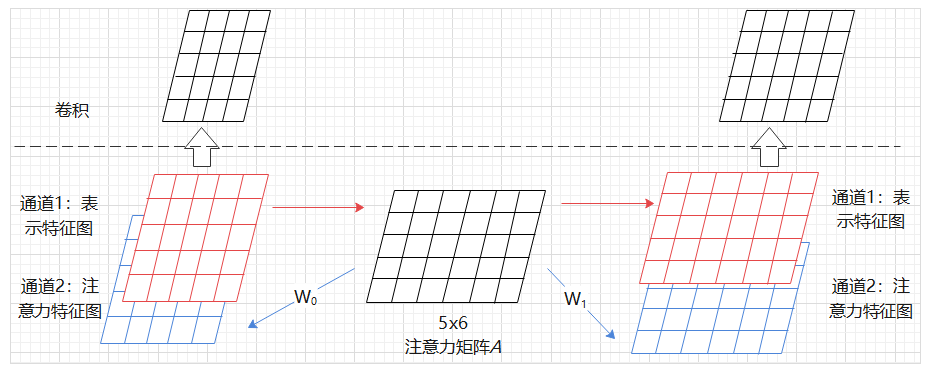
\includegraphics[width=5.6in]{figures/abcnn1.png}
\caption{卷积前注意力方案ABCNN-1}
\label{fig:abcnn1}
\end{center}
\end{figure}
\subsubsection{卷积后注意力方案}
相比ABCCN-1,卷积后注意力方案是针对卷积结果计算注意力矩阵,然后分行求和和分列求和求出加权向量,对于前提句第$i$个词,其权重是:
$$
\alpha_i=\sum_{j}a_{i,j}
$$
对于假设句第$j$个词,其权重是:
$$
\beta_j=\sum_{i}a_{i,j}
$$
模型会将卷积的结果乘上对应句子的权重,之后进行均值池化, 作为下一层的输入。网络的记过如图\ref{fig:abcnn2}所示。
\begin{figure}[h]
\begin{center}
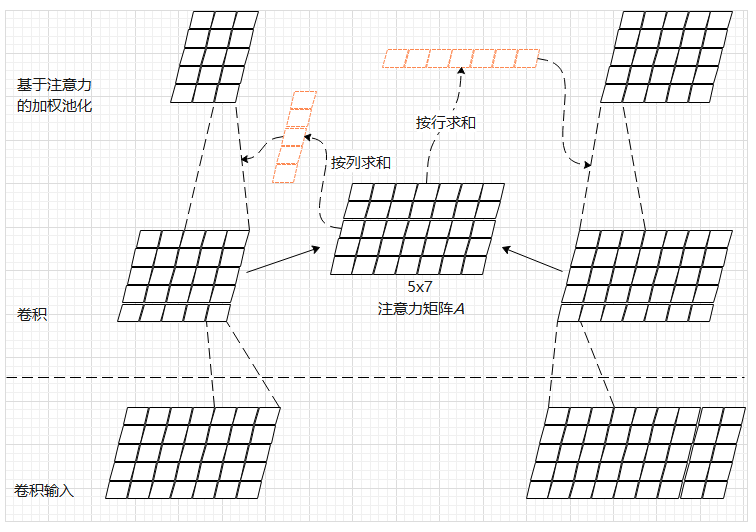
\includegraphics[width=6.0in]{figures/abcnn2.png}
\caption{卷积前注意力方案ABCNN-2}
\label{fig:abcnn2}
\end{center}
\end{figure}

\subsubsection{卷积前注意力和卷积后注意力加权结合方案}
\begin{figure}[h]
	\begin{center}
		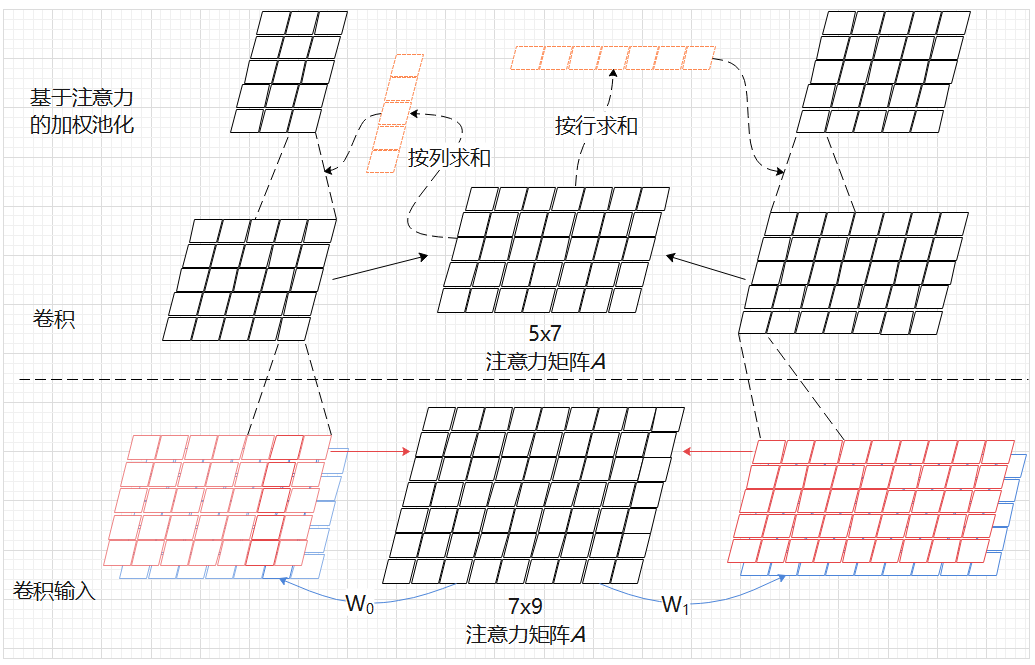
\includegraphics[width=6.0in]{figures/abcnn3.png}
		\caption{卷积前后同时注意力方案ABCNN-3}
		\label{fig:abcnn3}
	\end{center}
\end{figure}
相比之前的两张网络,ABCNN-3同步在卷积输入前和输入后都引入了注意力机制,是综合前两个网络的优势的一种组合方案。

ABCNN是基于\gls{CNN}的注意力模型,由于\gls{CNN}是空间计算,没有时间上的依赖,因此表现出比较强的并行加速优势。ABCNN的效果不如后面会讲到的ESIM网络,不过其速度是明显更快的。网络的记过如图\ref{fig:abcnn3}所示。

\subsection{ESIM-增强LSTM模型}
\begin{figure}[h]
\begin{center}
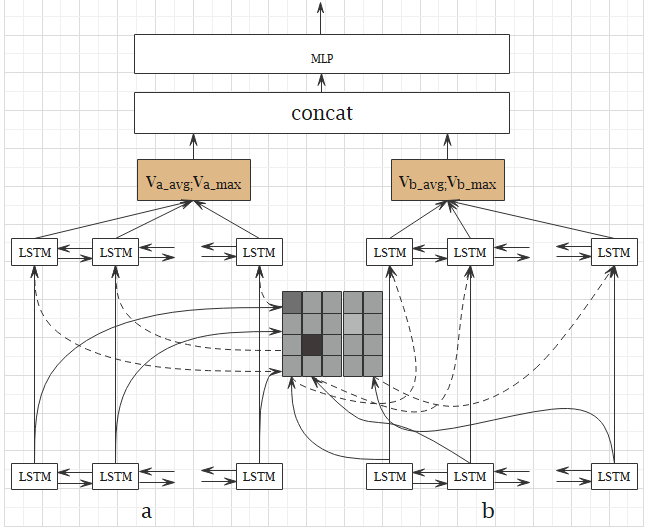
\includegraphics[width=5.6in]{figures/esim1.png}
\caption{ESIM网络结构}
\label{fig:esim1}
\end{center}
\end{figure}
在自然语言推理领域最具影响力的模型是ESIM模型,假定模型输入的两个句子为$a=[a_1,a_2,\cdots,a_n]$和$b=[b_1,b_2,\cdots,b_m]$,这个模型使用双向\gls{LSTM}进行句子编码:
$$
\begin{aligned}
\hat{a}_i = BiLSTM(a_i), \forall i \in [1,2,\cdots,n] \\
\hat{b}_i = BiLSTM(b_i), \forall i \in [1,2,\cdots,m]
\end{aligned}
$$
之后,我们会计算句子编码的交叉注意力,换言之,就是会将两个句子分别计算自己的语意在对方语意空间中的表示,具体做法如下:
$$
\begin{aligned}
\overline{a}_i &= \sum_{j=1}^m{
\frac{e_{i,j}}{\sum_{k=1}^n{e_{i,k}}}\hat b_j}, \forall i \in [1,2,\cdots,n] \\
\overline{b}_j &= \sum_{i=1}^n{\frac{e_{i,j}}{\sum_{k=1}^m{e_{k,j}}}\hat a_i}, \forall j \in [1,2,\cdots,m]
\end{aligned}
$$
其中,$e_{i,j}=\overline{a}_i^T\overline b_j$句子编码完成后模型会执行若干基本算术运算之后,将结果拼接起来
$$
\begin{aligned}
m_a&=[\hat a; \overline a; \overline a - \hat a; \overline a \odot \hat a]\\
m_b&=[\hat b; \overline b; \overline b - \hat b; \overline b \odot \hat b]\\
\end{aligned}
$$
后面$m_a$和$m_b$再经过一次BiLSTM:
$$
\begin{aligned}
v_a &= [BiLSTM(m_a;i), \forall i \in [1,2,\cdots,n]] \\
v_b &= [BiLSTM(m_b;i), \forall i \in [1,2,\cdots,m]]
\end{aligned}
$$
$v_a$和$v_b$经过一些pooling操作和拼接之后得到最终的语意表示
$$
v=[v_{a,avg};v_{a,max};v_{b,avg};v_{b,max}]
$$
最后经过若干层\gls{MLP}之后,就可以构建分类损失了。

句对分类技术还有很多其他的算法,不过目前看ESIM 算法是效果最好的。ESIM 算法最早用来解决自然语言推理问题,但是该网络在判断句子对语意相关性上也有比较强的应用前景, 我们在后续章节中会详细介绍语意搜索相关的课题。

\chapter{预训练技术}
在自然语言里面的预训练技术是指首先训练一个语言模型,然后在这个语言模型训练学习到的参数的基础上,根据不同的任务继续训练“微调”预训练语言模型学到的参数和学习任务特有的参数。预训练技术通常是两段式的学习,第一段学习的过程被称为“预训练”;第二段学习的过程被称为"微调"。第一阶段通常会学习一个语言模型,当然也有学习其他任务的,但是目前最为成熟的技术是训练语言模型。第二阶段任务通常称为下游任务,下游任务会有自己的独立参数。
\section{自然语言中预训练技术的发展历史}
在词向量训练出现的时候,人们就发现通过学到的词向量作为句子的Embedding矩阵,能够帮助自然语言处理任务提升指标。例如人们在研究\gls{CNN}在文本分类中的应用的时候,研究者就探讨了Embedding矩阵使用预先训练好词向量的作用,作者探讨了词向量在文本分类中的作用。作者在常见的7个数据集上分别使用随机初始化的词向量,预训练的词向量但是不做微调,和预训练的词向量并进行微调三种Embedding矩阵初始化方案,对比了效果,对比发现使用预训练的词向量并根据文本任务进行微调的方案,效果优于其他两种方案。预训练词向量并进行微调的技术,事实上已经称为现在自然语言处理领域的同行做法,人们现在已经将其广泛应用于文本分类、语义搜素和机器翻译等等诸多广泛的领域。

词向量的显著效果引起了研究人员的广泛关注,人们先后提出了多种改进方案,例如腾讯AI实验室提出的结合\gls{LDA}技术的有主题的词向量训练技术。
预训练技术的第一突破是Elmo的出现,Elmo 通过将句子语意上下文信息建模到词向量中,克服了传统词向量不考虑语境的问题。 简单来讲Elmo通过构建一个多层双向\gls{LSTM}语言模型来构建词汇的动态词向量,这个动态词向量的含义就是说同一个词在不同句子中数学表示不同。由于代码词向量的表示需要句子的上下文,因此Elmo训练语言模型的代码结构和学习过程中习得的参数必须被保留,这与传统的词向量已经产生了本质的不同,为此很自然的人们想到,可不可以在下游任务中继续微调Elmo模型涉及的参数呢?答案是肯定的。Elmo在不同的任务中均取得了不错的成绩,一度成为最流程的词向量模型,直到自注意力结构的出现,由于其颠覆式的表现,才逐步产生了取代Elmo的可能。

自注意力模型最早出现在机器翻译领域,用以改善翻译质量。最早的具有革命性意义的研究就是Google公司提出的Transformer模型,这个模型以其超群的表现,力压一众神经网络机器翻译模型,登顶Seq2seq领域的魁首。Transformer的成功引起了人们对Transformer对语意建模能力的关注,Google公司的一群研究人员,给Transformer的编码器接了一个巧妙设计的任务,希望借助这个模型来捕捉自然语言数学表达的奥妙。这个任务简单来讲就是从一篇文章中找出一些句子片段,将这些句子片段中的一些词给遮住,然后希望这个被遮住的部分能被其他部分通过Transformer的编码器变化后的数学特征预测出来。这个任务就是大名鼎鼎的掩码语言模型。当然也有其他人设计不同的任务给Transofmer的编码器,比如OpenAI设计的任务是传统的语言模型,他们的工作演变出著名的\gls{GPT}-x;微软公司的研究人员设计的是不同的任务
损失函数的和,也就是后来声名鹊起的MT-DNN。

这些基于自然语言注意力机制的预训练模型,刷新了人们对自然语言处理的认知,掀起了人工智能的新浪潮。在一些场景单纯的领域,计算机表现出来的智能水平,甚至达到甚至超越了人类。在预训练领域,除了自注意力模型之外,也有一些其他的研究,比如xlnet,号称超越了\gls{BERT},但是由于实现复杂,复现结果不稳定等因素难以复现等原因没有引起人们太多的注意力。

下面我们将介绍其中最具代表性的几种预训练模型。

\section{ELMo 多层RNN双向语言模型}
ELMo 多层\gls{RNN}双向语言模型首先是一个双向语言模型。给定$N$个符号表示一个句子$T=[t_1,t-2,\cdots,t_N]$,一个前向的语言模型计算的句子的重构概率,这个概率越高表示句子越通顺,否则表示句子越不通顺。
$$
p(t_1,t_2,\cdots,t_N)=\prod_{k=1}^N{p(t_k|t_1,t_2,\cdots,t_{k-1})}
$$
如前述章节介绍,目基于循环神经网络的语言模型,首先通过将句子中每个词的Embedding顺次输入一个$L$层的单向循环神经网络并通过隐层的输出$H_k^L$来建模上下文,并预测第$k$个词的出现概率:
$
p(t_k|t_1,t_2,\cdots,t_{k-1};\Theta_{forward}) 
$
那么前向语言模型的对数似然概率可以写成:
$$
\begin{aligned}
L(\Theta_{forward})&=log\prod_{k=1}^Np(t_k|t_1,t_2,\cdots,t_{k-1};\Theta_{forward}) \\
&=\sum_{k=1}^N{log(p(t_k|t_1,t_2,\cdots,t_{k-1};\Theta_{forward}))}
\end{aligned}
$$
同样的办法可以构建一个后向的语言模型,其对数似然概率可以写成:
$$
\begin{aligned}
L(\Theta_{backward})&=log(\prod_{k=1}^Np(t_k|t_1,t_2,\cdots,t_{k-1};\Theta_{backward}) \\
&=\sum_{k=1}^N{log(p(t_k|t_1,t_2,\cdots,t_{k-1};\Theta_{backward}))}
\end{aligned}
$$
我们把正向损失和反向损失加在一起就得到了一个双向语言模型:
$$
\begin{aligned}
L(\Theta_{backward},\Theta_{forward}) 
&= \sum_{k=1}^N 
(
    log(p(t_k|t_1,t_2,\cdots,t_{k-1};\Theta_{backward})) \\
& + log(p(t_k|t_1,t_2,\cdots,t_{k-1};\Theta_{backward}))
)
\end{aligned}
$$
\begin{figure}[htbp]
\begin{center}
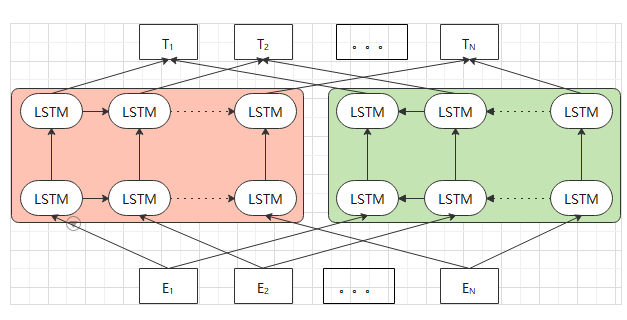
\includegraphics[width=5.6in]{figures/elmo1.png}
\caption{ELMO网络结构}
\label{fig:elmo1}
\end{center}
\end{figure}


在训练下游任务的时候,会把双向语言模型中各个循环神经网络的隐层输入$\{[\overleftarrow{ H_{l}},\overrightarrow{ H_{l}}]|l=1,2,\cdots,L\}$和语言模型输入的Embedding矩阵$X$组合起来计算一个向量序列作为词的上下文表示。可以有多种使用方法,例如直接线性加权或者只取最上层的输出。ELMo在问答、自然语言推理、命名实体识别和文本分类等诸多数据集上刷新了当时的最高水平,展现出非常高的实用价值。

\section{BERT}
近几年最能代表自然语言处理技术的水平的非\gls{BERT}莫属,\gls{BERT}是一种双向语言模型,\gls{BERT}使用了Transformer 翻译模型的编码端,我们来详细介绍这个编码端的结构。

\gls{BERT}弃用了\gls{RNN},因此无法建模句子的位置信息,\gls{BERT}引入了位置编码,具体来讲就是给每个位置随机生成一个可训练的向量$P_i$,然后和词向量$W_i$加在一起作为模型的输入。
$$
X_i = P_i + W_i
$$
我们看代码, 这段代码首先生成两个占位变量x和x\_mask,用来存放模型的输入。其中x用来存放句子的ID序列,由于同一batch中有些句子长有些句子短,但是张量的最后一列必须是定长的,所以我们需要做补零操作,例如batch\_size为3的一组输入如下:
$$
\begin{aligned}
\text{x} = \left [
\begin{matrix}
1,2,3,4 \\
5,6,0,0 \\
7,8,9,0
\end{matrix} \right ], &
\text{x\_mask} = \left [
\begin{matrix}
1,1,1,1 \\
1,1,0,0 \\
1,1,1,0
\end{matrix} \right ]
\end{aligned}
$$
\begin{lstlisting}[language={Python}]
def create_input_layer(batch_size, max_seq_len, vocab_size, hidden_size):
    """ 
    构建输入层 
    """
    embedding_size = hidden_size
    x = tf.placeholder(dtype=tf.float32, shape=[batch_size, max_seq_len])
    x_mask = tf.place_holder(dtype=tf.float32, shape=[batch_size, max_seq_len])
    embedding_table = tf.get_variable([vocab_size, embedding_size],
        name = "word_embedding_name",
        shape = [vocab_size, embedding_size],
               initializer = tf.truncated_normal_initializer(stddev=0.02))
    pos_embedding_table = tf.get_variable([max_seq_len, embedding_size],
        name = "pos_embedding_name",
        shape = [vocab_size, embedding_size],
               initializer = tf.truncated_normal_initializer(stddev=0.02))
    x_embedding = tf.nn.embedding_lookup(params=embedding_table, ids=x)
    x_pos_embedding = tf.slice(input_=pos_embedding_table, begin=0, size=max_seq_len)

    return x_embedding + x_pos_embedding, x, x_mask
\end{lstlisting}
\subsection{多头注意力层}
模型的输入首先输入层后,会经过一个多头自注意力层。多头注意力层操作的具体做法是首先将$X$通过线性变换运算变换到三个维度为$H/k$的低纬度空间,:
$$
\begin{aligned}
Q_j = W_{Q_j}X\\
K_j = W_{K_j}X\\
V_j = W_{V_j}X
\end{aligned}
$$
其中$H$为Embedding层输入维度,$k$是一个正整数。然后计算这个低纬度空间里面的注意力作为输出
$$
\hat{X_j} = softmax(\frac{Q_jK_j^T}{\sqrt{H/k}})V_j
$$
之后将这些低纬度的输出拼接起来就得到了多头注意力机制的最终输出
$$
\hat{X} = [\hat{X_1};\hat{X_2};\cdots;\hat{X_k}]W_o
$$
\begin{figure}[htbp]
\begin{center}
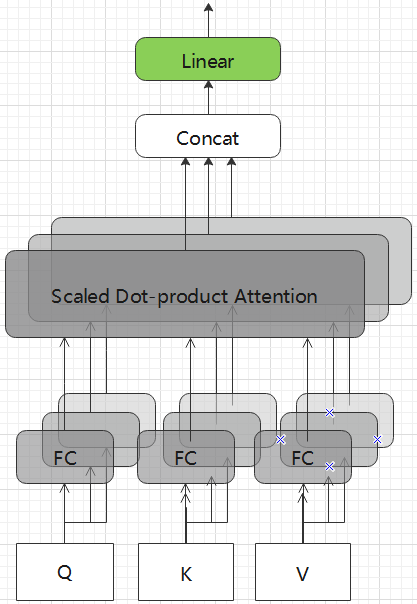
\includegraphics[width=4.0in]{figures/bert1.png}
\caption{多头注意力机制}
\label{fig:bert1}
\end{center}
\end{figure}

最后我们来看看代码,代码面前无密码:

\begin{lstlisting}[language={Python}]
def multi_head_attention(x_embedding, x_mask, hidden_size, head_num, attention_future=True):

    def attention_mask_before_softmax(matrix, from_mask, to_mask, attention_future=True):
        """
        通过加一个非常小的数,保证在softmax的时候,对应位置变成0
        """
        to_mask = tf.cast(x=to_mask, dtype=tf.float32)
        attention_adder = (1.0 - tf.expand_dims(input=to_mask, axis=1)) * (-2.0 ** 31 + 1.0)

        if attention_future == False:
            mask_matrix = tf.ones_like(matrix[0], dtype=tf.float32)
            mask_matrix = 1.0 - tf.linalg.band_part(input=mask_matrix, num_lower=-1, num_upper=0)
            mask_matrix = tf.expand_dims(input=mask_matrix, axis=0) * (-2.0 ** 31 + 1.0)
            matrix = matrix + mask_matrix  # here the first dimision will be broadcast

        return matrix + attention_adder  # here attention_adder will be broadcast according to axis 1
    heads = list()
    for i in range(head_num):
        Q = tf.layers.dense(use_bias=False, name='Q'+str(i), inputs=x_embedding, units=hidden_size/head_num)
        K = tf.layers.dense(use_bias=False, name='K'+str(i), inputs=x_embedding, units=hidden_size/head_num)
        V = tf.layers.dense(use_bias=False, name='V'+str(i), inputs=x_embedding, units=hidden_size/head_num)

        dot_product = tf.matmul(a=Q, b=K, transpose_b=True)
        dot_product = attention_mask_before_softmax(matrix=dot_product, from_mask=x_mask, to_mask=x_mask)
        dk = tf.cast(x=hidden_size/head_num, dtype=tf.float32)
        tf.sqrt(dk)
        coordinate = tf.nn.softmax(logits=dot_product/dk, axis=1)
        head = tf.matmul(a=coordinate, b=V)
        heads.append(head)
    
    concat_heads = tf.concat(values=heads, axis=-1)
    ret = tf.layers.dense(use_bias=False, name='multi-head-attention-project', inputs=concat_heads, units=hidden_size)
    return ret
\end{lstlisting}

\subsection{残差连接、规范化和高维投射}
完成多头注意力操作之后,\gls{BERT}会加上残差连接后会将模型经过残差连接后投射到一个高维空间,然后在通过线性变换转换到和隐藏层维度相同的空间。这些操作我们称之为注意力辅助层。我们来看代码:

\begin{lstlisting}[language={Python}]
def  assist_layer(x_hidden, x_mask, width_hidden_size, hidden_size):

    x_hidden = tf.multiply(x=x_hidden, y=x_mask)
    x_project = tf.layers.dense(inputs=x_hidden, name="project-1", units=width_hidden_size, 
                                use_bias=True, activation=tf.nn.relu)
    x_mask_hidden = tf.expand_dims(input=x_mask, axis=-1) # batch_size x max_seq_len x 1
    x_project = tf.multiply(x=x_project, y=x_mask_hidden)
    x_output = tf.layers.dense(inputs=x_project, name='project-2', units=hidden_size)
    x_output = tf.multiply(x=x_output, y=x_mask_hidden)
\end{lstlisting}

\gls{BERT}就是反复堆叠若干组多头注意力层和和注意力辅助层最后接上损失函数就可以训练了。其中一组多头注意力和和注意力辅助层被称为一个Transformer模块,下面我们给出网络结构构建的核心代码:
\begin{lstlisting}
class BertModel:
    
    def __init__(self, layer_num, config):
        
        self.layer_num = layer_num
        self.config = config

    def __add_norm(self, x_hidden, x_prev_hidden):
        
        x_hidden = x_hidden + x_prev_hidden
        tf.contrib.layers.layer_norm(inputs=x_hidden)

    def create_model(self):
        
        batch_size = self._config.batch_size
        max_seq_len = self._config.max_seq_len
        vocab_size = self._config.vocab_size
        hidden_size = self._config.hidden_size
        width_hidden_size = self._config.width_hidden_size
        head_num = self._config.head_num
        x_input, x, x_mask = create_input_layer(batch_size, max_seq_len, vocab_size, hidden_size)
        for i in range(self.layer_num):
            x_hidden = multi_head_attention(x_embedding=x_input, x_mask=x_mask,
                                            hidden_size=hidden_size, head_num=head_num)
            x_hidden = self.__add_norm(x_hidden=x_hidden, x_prev_hidden=x_input)
            x_project = assist_layer(x_hidden=x_hidden, x_mask=x_mask,
                                     width_hidden_size=width_hidden_size, hidden_size=hidden_size)
            x_project = self.__add_norm(x_hidden=x_project, x_prev_hidden=x_hidden)
            x_input = x_project
        
        return x_input
\end{lstlisting}
需要注意的是其中有一个函数\_\_add\_norm 这个函数实现了残差连接之外还增加了一个层内归一化,保证输入输出的分布大致一致。最后需要强调的,\gls{BERT}论文中讲到了几处dropout,我们这里为了突出模型的主体结构没有在代码中加入,读者如果需要实战的化,建议阅读一下论文,把这些正则化的操作都加上。
\subsection{掩码语言模型-MLM}
\gls{BERT}的网络结构可以理解为是对句子表示的一种建模方式,下面我们来介绍\gls{BERT}的学习任务,\gls{BERT}在预训练阶段使用了掩码语言模型作为训练任务。这个任务的输入是一个句子,然后从句子中随机挑选一部分词,并将这部分词用掩码掩掉,用剩下没有掩掉的词来预测被掩码掉的词,如图\ref{fig:bert2}所示,Bert的整体网络结构如图\ref{fig:bert2}所示。
\begin{figure}[!h]
\begin{center}
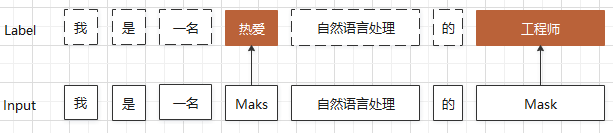
\includegraphics[width=5.6in]{figures/bert2.png}
\caption{BERT掩码语言模型的样本构建方法}
\label{fig:bert2}
\end{center}
\end{figure}
\begin{figure}[h]
	\begin{center}
		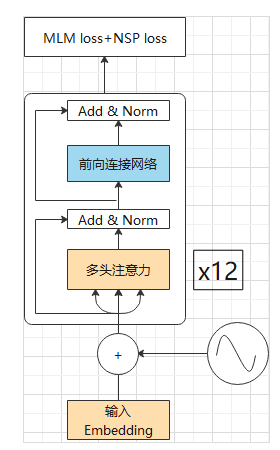
\includegraphics[width=3.5in]{figures/bert3.png}
		\caption{\gls{BERT}预训练网络结构}
		\label{fig:bert2}
	\end{center}
\end{figure}


需要强调的是\gls{BERT}原始论文中的还有一个NSP任务,但是后续的研究表明,去掉NSP任务后预训练的效果并没有打折扣,所以我们这里引入\gls{BERT}模型的时候,并没有介绍这部分内容。另外建议大家使用动态掩码技术,具体来讲就是不要在构造训练集的时候指定mask的位置,因为这样一来不同的epoch中同一个句子的mask位置固定,而要在构建batch的时候使用随机数动态生成需要mask的位置,这样一来就可以克服上述问题。Facebook的研究人员增加了上述改造后,对比原始的\gls{BERT},在GLUE任务上取得了进一步的提升。
\subsection{BERT的下游任务训练}
\gls{BERT}是一种预训练技术,首先将模型训练好后,通过迁移学习将学习好的参数应用到下游任务中。对于分类任务,\gls{BERT}通常取[CLS]对应的隐藏层输出后通过线性映射直接预测目标分类,单句分类和句对分类任务均可采用这种方法;对于答案抽取式的阅读理解,只要对上下文的每个输入对应的隐层输出预测其作为答案开始或者结束的概率即可;对于\gls{NER}等序列标注任务,只需要对每个输入的隐藏层输出通过线性映射后预测其作为标签集合中任一元素的概率即可。如图\ref{fig:bert3}所示。

	\begin{figure}[htbp]
		\centering
		\subfigure[句对分类任务]{
			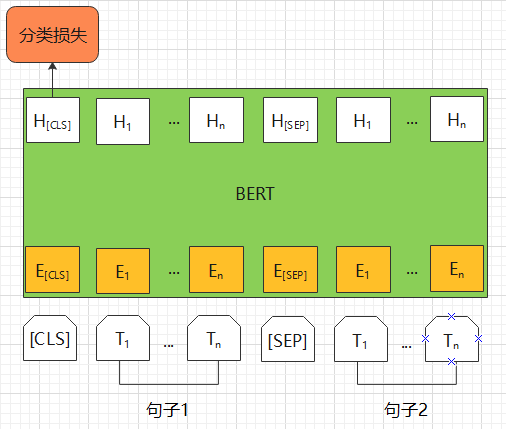
\includegraphics[width=0.45\textwidth]{figures/bert_f1.png}
		}
		\subfigure[单句分类任务]{
			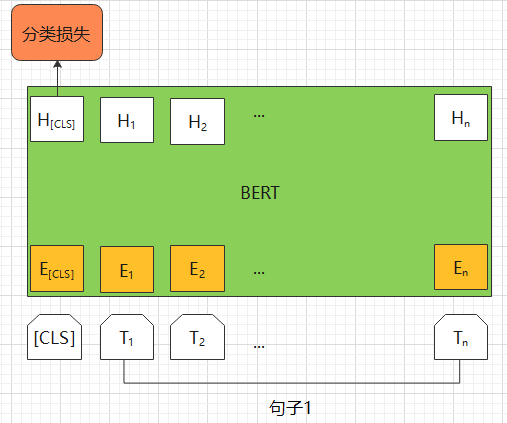
\includegraphics[width=0.45\textwidth]{figures/bert_f2.png}
		}
		\subfigure[问答任务]{
			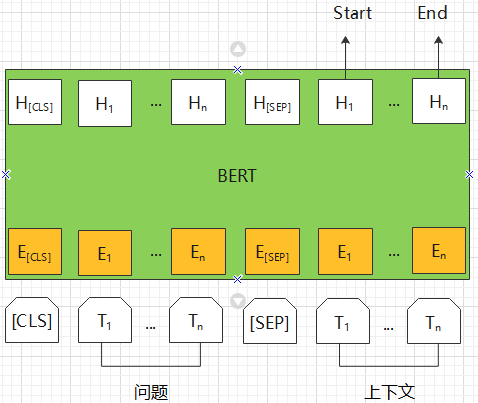
\includegraphics[width=0.45\textwidth]{figures/bert_f3.png}
		}
		\subfigure[序列标注任务]{
			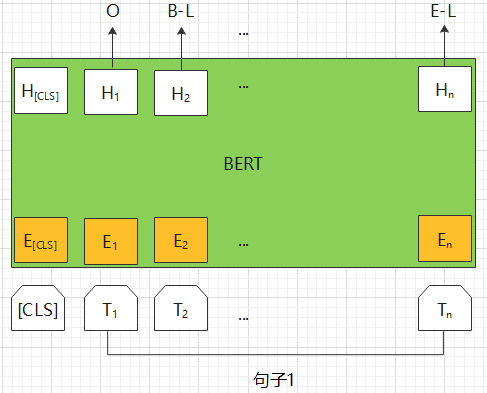
\includegraphics[width=0.45\textwidth]{figures/bert_f4.png}
		}
		\caption{BERT的下游任务训练}
		\label{fig:bert3}
	\end{figure}

\section{MTDNN}
在\gls{BERT}出现后,微软公司的一些研究者提出了基于Transformer编码器作为特征表示的多任务预训练模型--\gls{MTDNN}。与\gls{BERT}类似,\gls{MTDNN}使用多层Transformer模块堆叠作为文本特征提取网络,希望能够借助注意力机制得到更好的文本表示。与\gls{BERT}不同的是,\gls{MTDNN}在构建预训练任务的时候,不是使用掩码语言模型,而是非常暴力的使用很多任务。在微软公司的研究者看来,计算机应该像人一样能把一个任务学习到的任务应用到另一个任务中。我把这种生物认知现象称为认知迁移,微软的研究人员希望模型能够捕捉到认知迁移的内在规律在自然语言处理中的表现形式。如图所示\gls{MTDNN}接入了四种任务。 这四个任务分别是单文本分类任务、文本相似度任务、句子对文本分类任务和语意相关性搜索任务。\gls{MTDNN} 的输入和\gls{BERT} 是一样的,每个句子的输入都会增加一个起始符号[CLS],如果输入是一个句子对那么两个句子用[SEP]这个特殊符号分割,假定文本输入的输出为$l_2$。
\begin{example}
假如输入是"我是一个自然语言处理工程师"这一个句子,那么\gls{MTDNN}的输入是"[CLS]我是一个自然语言处理工程师";假如输入是"我是一个自然语言处理工程师"和"我热爱自然语言处理",那么\gls{MTDNN}的输入就是"[CLS]我是一个自然语言处理工程师[SEP]我热爱自然语言处理"。
\end{example}
\begin{figure}[htbp]
\begin{center}
\includegraphics[width=5.8in]{figures/mtdnn1.png}
\caption{MTDNN网络结构}
\label{fig:mtdnn1}
\end{center}
\end{figure}

\subsection{单句分类任务}
假定$X$是文本上下文序列编码$l_2$的第一个字符[CLS]的文本编码,与\gls{BERT}类似,我们使用$X$作为文本的语意表示。这里文本的语意表示,如果是单句分类为$X_1$的语意表示,如果是句子对分类是$[X_1;X_2]$的语意表示。那么$X$被分到$c$类别的概率为:
$$
P_{SST}(c|X)= softmax(XW_{SST})
$$
在\gls{MTDNN}中采用了交叉熵损失作为优化目标,对于其中的一个样本:
$$
L_{SST}=-\sum_{c}I(X,c)log(P_{SST}(c|X))
$$。
\subsection{句子对分类任务}
我们前面章节讲过句子对分类任务,\gls{MTDNN}的模型在构建句对分类损失的时候使用了\gls{SAN} 网络的回答模块来构造文本的语意表示,这方面的内容比较复杂,具体请参考后续章节中,讲机器阅读理解的章节。不过在构造损失函数的时候,\gls{MTDNN}模型的处理方式与单文本分类没有区别。

\subsection{文本相似度任务}
假定$X$是文本上下文序列编码$l_2$的第一个字符[CLS]的文本编码,那么我们将$X$视作是句子对$[X_1;X_2]$的语意编码,我们定义这两个句子对的相似度为:
$$
sim(X_1,X_2) = XW_{STS}
$$
在\gls{MTDNN}中采用了均方误差作为优化目标,对于其中的一个样本:
$$
L_{STS}=(y-sim(X_1,X_2))^2
$$
\subsection{语意相关性搜索任务}

\gls{MTDNN}通过对QNLI任务的正样本做了一个负采样,将其构建成了一个语意相关性排序的任务,其中查询句$Q$和回答句$A$的相关性得分为:
$$
Rel(Q,A) = g(XW^T_{QNLI})
$$
其损失函数采用了pairwise-learning-rank的思路, 对于其中的一个样本的损失定义为:
$$
\begin{aligned}
L_{QNLI} &= \sum_{(Q,A^+)}P(A^+|Q)\\
P(A^+|Q) &= \frac{exp(Rel(Q,A^+)}{\sum_{A}exp(Rel(Q,A))}	
\end{aligned}
$$
其中$A^+$表示正样本。

\gls{MTDNN}的训练流程是比较直接的,Transformer层采用\gls{BERT}预训练的参数来初始化自己的参数;在构造特征的阶段四个任务分别组成各自的batch:$B_{SST}, B_{STS}, B_{QNLI}, B_{SP}$,之后将其合并成一个大的batch:$B = shuffle([B_{SST}, B_{STS}, B_{QNLI}, B_{SP}])$。在计算损失阶段,根据任务数据计算不同的损失后,将这些结果加起来就是最后的损失。最后需要强调一下,这些任务的共享了Transformer部分的参数。
\subsection{总结}
目前看\gls{BERT}依然吸引了绝大部分研究和应用的目光,\gls{MTDNN} 原始论文中使用的是GLUE数据集,其实很多语言的GLUE数据集并不完整,例如中文的GLUE数据集就没有英文完整,所以也限制了\gls{MTDNN}的应用范围。另外\gls{MTDNN}相对\gls{BERT}的提升并没有表现出绝对优势,后来Facebook的研究人员对\gls{BERT}稍加改动之后,又反超了\gls{MTDNN}。我个人的建议是,读者可以把\gls{MTDNN}当成一种学习和参考的思路,不大建议投入过多的研究或者尝试将其引入到工业应用中来。

\section{精简BERT模型ALBERT}
近些年来,预训练语言模型的参数量越来越大,BERT-Base目前的参数量已经超过100M,因此训练代价和使用代价也越来越大。ALBERT就应运而生了,ALBERT 要解决的第一个问题就是参数量问题,解决的办法主要有两方面:一方面通过矩阵分解的方法来降低embedding矩阵的大小;另一方面是使用跨层参数共享的方法来降低隐藏层的参数量。
\subsection{Embedding 矩阵的分解}
研究表明Embedding矩阵的参数量约占整个模型参数量的$20\%$以上,造成这个主要原因有两方面:一是词表巨大,二是Embedding矩阵的列维度太大。在\gls{BERT} 中一般要求Embedding的维度$E$和模型的隐藏层维度$H$相等,一般认为模型的隐藏层的输出是上下文相关的语意表示,而Embedding层的输出是上下文无关的语意表示。研究表明\gls{BERT}等模型的威力主要来自于上下文相关的语意,那我们有没有可能解耦隐藏层和Embedding层,并使得$E<<H$呢?在数学上我们可以通过把一个矩阵分解成连个矩阵的乘积形式
$$
M_{V \times H}=Q_{V \times C}R_{C \times H}
$$
如果$C<<H$,那么$M_{V \times H}$的元素数量远远大于$Q_{V \times C}R_{C \times H}$的参数量,因为如果$H>>C$,则$V\times H >> V \times C + C \times H$。

\subsection{跨层参数共享}
ALBERT 希望通过跨层参数共享来提高参数的利用率,事实上参数共享的方式非常多,比如可以仅仅共享注意力计算层,或者仅仅共享前向高维映射层等。ALBERT的处理方法非常暴力,就是共享所有的参数。如果层数为$N$,那么这种共享方法可以直接将参数量压缩到原来的$1/N$。需要强调的是ALBERT因为参数量少,梯度更新速度会更快,但是由于ALBERT本质上没有改变前向传播的计算过程,因此其推理速度从理论上看,并不会有太多的下降。


\section{其他预训练技术}
\begin{figure}[htbp]
\begin{center}
\includegraphics[width=5.8in]{figures/ernie1.png}
\caption{ERNIE相对BERT的改进}
\label{fig:ernie1}
\end{center}
\end{figure}
其实工业界和学术界针对\gls{BERT}存在的缺点,进行了诸多改进。其中比较有名的改动是百度的ERNIE,这个预训练模型宣称在中文的很多任务上超越了\gls{BERT}。ERNIE 认为\gls{BERT}存在两个问题,第一个问题是\gls{BERT}在中文预训练中只能做到汉字级别的mask。在下面的例子中,\gls{BERT}就把“哈尔滨”这个词的“尔”字单独mask作为了label,其实我们知道“哈尔滨”是黑龙江省的省会,是一个城市名,单独将“尔”字拆出来并无特别意义;第二个问题是ERNIE认为\gls{BERT}在中文预训练的时候使用的语料过于单一,当然这个有一点牵强,事实上,\gls{BERT}本身并不限制所用的训练语料。为了解决这两个问题,ERNIE在训练语料中引入了实体概念等先验知识,对词和实体概念等语义单元进行 mask,避免了实体语意被mask分割掉。另外ERNIE引入了多源训练语料,特别是引入了社区对话语料,来克服单一百科数据的数据准备不足的问题。除了ERNIE之外,最负盛名的就是XLNET了,这个模型提出了排列语言模型,并宣称在很多数据集上超越了\gls{BERT},但是从我个人的实践经验看来,对这项技术还要需要持观望态度,大家有兴趣可以自行阅读相关的论文。


\chapter{序列标注}

序列标注任务是非常著名的自然语言处理任务,是分词、词性标注和命名实体识别等关键任务的基础技术。在深度学习兴起之前,人们已经开始使用统计机器学习的方法来解决序列分类问题,其中最具代表性的技术是\gls{HMM}和\gls{CRF}。前者是一种生成任务,后者是一种判别任务。后来深度学习逐渐兴起,研究者发现深度学和\gls{CRF}的结合,具有超乎想象的效果提升,后来\gls{BERT}和\gls{CRF}的结合已经将公开数据集的准确度刷新到非常高的水平。目前的研究已经基本停滞,近几年也没有什么特别亮眼的成果。近几年的比较有影响力的论文当属《Hierarchically-Refined Label Attention Network for Sequence Labeling》,这篇论文提出一种比较新鲜的思路,有一定的借鉴意义。

\section{序列标注任务}
序列标注任务是就是给定一个句子,$X=x_1,x_2,\cdots,x_n$,我们称之为输入序列;这个序列的每个位置都有一个标签,$Y=y_1,y_2,\cdots,y_n$,我们称之为标签序列。序列标注任务就是根据给定的输入序列来预测标签序列。序列标注任务要求输入序列和标签序列是等长序列。常见的任务例如分词、命名实体识别和事件抽取等任务,都可以建模成标注任务。对于分词任务,我们的输入序列是一个完整的句子,例如“我是一个热爱自然语言处理的工程师”,如果我们能够预测出一个标注序列为"BBBIBIBIIIIIBBII",那么我们就可以根据这个标注序列将输入序列进行分词,我们每碰到一个B字符就认为是一个新词的开始,直到碰到下一个B字母或者句子结束。值得注意的是如果句首出现I字符我们也认为是新词的开始,这样可以证明任何标注序列都可以构造出一个分词序列。另一个著名的序列标注任务是命名实体识别任务,所谓命名实体是指人名、机构名、地名以及其他所有以名称为标识的实体。更广泛的实体还包括数字、日期、货币、地址等等。命名实体识别就是从一段给定的输入序列中找到是命名实体对应的位置,例如下面的例子中存在一个机构名——北京大学和一个人名。我们使用BIO首字母后面跟一个表示实体类别的标签来区分不同的实体类型,例如B-P表示一个人名的开始,B-L表示一个地名的开始。通常来说序列标注任务中同一个实体不可能既是人名又是地名的,如果把非实体位置用O标记那么可以保证输入序列和输出序列的长度是等长的。
\begin{table}[h]
	\caption{序列标注任务举例}  
	\centering
	\scalebox{0.9}{
		\begin{tabular}{l|llllllllllllllllllll}
		  \toprule
		  \midrule
		   	输入序列&鲁&迅&曾&经&在&北&京&大&学&学&习\\
		  \midrule
			标签序列&B-P&I-P&O&O&O&B-L&I-L&I-L&I-L&O&O\\
 		  \bottomrule
		\end{tabular}
	}
\end{table}

序列标注任务除了BIO标注法之外也常用BMES标注法,我们在分词那一章已经介绍过这两种标注方法。

\section{条件随机场}
在深度学习兴起之前,人们在解决序列标注任务的时候,使用最多且效果最好的非条件随机场莫属。条件随机场是指给定一组输入随机变量$X$的条件下另一组输出随机变量$Y$的马尔可夫随机场,对于分词任务$X$可以理解为输入序列,$Y$可以理解为输出序列。马尔科夫随机场是一种特殊的随机场,简单来讲就是随机场具有马尔科夫性。
\subsection{线性链马尔科夫条件随机场}
要理解马尔科夫随机场,必须先理解随机场的概念。随机场是指在一个空间中分布的一组相互作用的随机变量。在序列标注任务中,随机场的空间就是一条线性链,在这条线性链中分布着一系列的随机变量,这些随机变量相互作用就组成一条线性链上的随机场,这种随机场我们也称为线性链随机场。假定这条链上的随机变量仅和周围的一个长度为$l$的对称窗口里的其他变量有关系那么我们称这条线性链上的随机变量具有马尔科夫性,称为线性链马尔科夫随机场。假定存在一个随机序列$X=x_1,x_2,\cdots,x_n$,在这个序列的某个取值序列发生的条件下,另一个与之相关的等长的随机序列$Y=y_1,y_2,\cdots,y_n$是马尔科夫随机场,那么这个随机系统被称为线性链马尔科夫条件随机场简称条件随机场。用数学的语言描述就是,$y_i$的条件概率分布满足:
$$
P(y_i|X,y_1,y_2,\cdots ,y_{i-1},y_{i+1},y_{i+2},\cdots ,y_n)=
P(y_i|X,y_{i-l},\cdots ,y_{i-1},y_{i+1},\cdots,y_{i+l})
$$
一般来说条件窗口的长度$l$一般取1,以简化问题的复杂度。
\subsection{条件随机场的学习问题}
条件随机场的学习问题是指求条件随机场关键参数的过程,具体来说就是求决定概率取值
$
P(Y|X)=f(X,Y,\Theta)
$
的参数$\Theta$ 的求解过程。根据线性链条件随机场的定义,可以推知决定$P(Y|X)$取值的因素包括三类:
第一类我们称为点因素或者点特征,第二类我们称为前向边因素或者前向边特征,第三类特征我们称为后向边因素或者后向边特征。如图所示,点特征建模$x_i$对$y_i$的概率转移特征,我们记为$v_k(y_i,X,i)$,前向边特征建模$y_{i-1}$和$y_{i}$的概率转移特征,我们记为$f_k(y_{i-1},y_i,X,i)$,后向边特征建模$y_{i}$和$y_{i+1}$的概率转移特征,我们记为$b_k(y_{i},y_{i+1},X,i)$。条件随机场在应用的时候做了一个假定,我们假定$P(Y|X)$具备如下形式:
$$
\begin{aligned}
P(Y|X)  =
\frac{1
}{
Z(X)
}
exp(\sum_{i,k}(\alpha _i v_k(y_i,X,i))\\
	+\sum_{i,k}(\beta _i f_k(y_{i-1},y_i, X,i))\\
	+\sum_{i,k}(\gamma _i b_k(y_{i},y_{i+1},X,i)))\\
\end{aligned}
$$
其中,
$$
Z(X) = \sum_{Y}exp(\sum_{i,k}(\alpha _i v_k(y_i,X,i)+\beta _i f_k(y_{i-1},y_i, X,i)+\gamma _if_k(y_{i},y_{i+1},X,i)))
$$
一般来说,点特征和边特征都是描述一种共现现象是否出现,例如在分词任务中点特征可以用来描述"我"字和"B"的共现。可以用点特征为$t(B,\text{我})=1$来表示\text{我}字出现为词首的现象。需要强调的是这些特征需要自己定义,不过一些常见的任务,人们都已经摸索出比较有效的特征定义模板,可供参考,大家不用烦恼如何选取特征的问题了。

至此我们已经可以把序列标注问题建模成了一个参数估计问题了,这个参数的估计问题可以使用很多方法,例如可以使用基于极大似然估计的梯度下降法。不明白极大似然估计的同学,本人推荐大家下学习一下概率论相关的知识。需要强调的是计算$Z(X)$需要枚举$Y$的所有可能序列,这是一个有重序列的排列生成问题,需要比较大的计算代价,因此需要一些计算技巧。不过从原理上讲,这些内容和理解条件随机场本身没有关系。到目前为止我们已经掌握了如何计算条件概率$P(Y|X)$了,从数学上我们可以通过枚举所有可能的$Y$的取值然后比较之后,求使得$P(Y|X)$概率最大的$Y$就可以了,不过大家都知道枚举$Y$的所有可能是排列生成问题,这个问题时间复杂度是惊人的,这也是为什么在条件随机场上添加马尔科夫限制的原因。因此如果模型参数已知,我们就能使用维特比算法来规划求解条件随机场的解码问题了。

\subsection{条件随机场的解码问题}
\begin{definition}
条件随机场的解码问题就是我们已经知道条件随机场的的模型参数$\Theta$,给定输入序列,求出最佳标签序列的问题,所谓最佳标签序列就是已知输入序列$X$使得概率值$P(Y|X)$最大的标签序列$Y$。
\end{definition}
这个算法可以分三步走,第一步考虑点特征和前向边特征,从左到右扫描到当前位置$i$,计算以$y_i$结尾的标注序列出现的最大概率$P(*y_i|X[:i])$,我们把这个概率序列称为前向概率序列,对于前向概率序列的第$i$项,我们仅考虑前向边特征和点特征对当前项的影响,也就是说仅仅与前向概率序列的第$i-1$项有关,因此具有如下的地推公式:
$$
P(*y_i|X[:i])=max_{y_{i-1}}{(P(*y_{i-1}|X[:i-1]) + \sum_{k}(\beta_i b_k(y_{i-1},y_i, X,i)))}
$$
第二步我们计算后向概率序列,所谓后向概率序列是指仅仅考虑点特征和后向边特征,计算从右向左扫描到当前位置$j$,计算以$y_j$打头的标注序列出现的最大概率$P(y_j*|X[j:])$。计算方法和前向概率序列的计算公式类似:

$$
P(y_j*|X[j:])=max_{y_{j+1}}{(P(y_{j+1}*|X[j+1:]) + \sum_{k}\beta_i f_k(y_{j+1},y_i, X,j))}
$$
第三步,我们同步考察左右两边的影响,对于第$i$个位置
$$
P(y_i*|X[i:])=\max_{y_{i-1};y_{i+1}}P(*y_{i-1}|X[:i-1])\sum_{k}\alpha_i v_k(y_i, X,i)P(*y_{i+1}|X[i+1:]))
$$
我们这里每个位置的不同特征共享了权重,也就是说同一个位置的权重$\alpha_i$与这个位置的点特征函数$v_k$、前向边特征$f_k$和后向边特征$b_k$没有关系,因此我们成这种现象为共享权重;当然权重也可以不共享,以提升模型的表达自由度,不过不共享权重会造成模型规模膨胀。

\section{基于循环神经网络和CRF结合的序列标注算法}
循环神经网络隐藏层的输出序列可以理解为一种上下文相关的词向量,一个直观的想法是,在词向量的输出后面接一个线性映射层后经过softmax 直接构造序列标注任务的损失。这种构造方法没有建模标签序列的转换约束限制,例如I-L标签不能在O标签之后。为了解决直接使用softmax构建损失是没办法构建标签转变约束的这个问题,研究人员引入了\gls{CRF} 损失函数。模型的结构如图\ref{fig:bilstm-crf1} 所示。
\begin{figure}[htbp]
\begin{center}
\includegraphics[width=5.6in]{figures/bilstm-crf1.png}
\caption{BiLSTM + CRF}
\label{fig:bilstm-crf1}
\end{center}
\end{figure}

为了讲清楚\gls{CRF}损失函数的构建过程,我们首先定义一些变量:我们定义标签序列的取值集合为$T=\{t_1,t_2,\cdots,t_{|T|}\}$, 一个给定的输入序列对应的BiLSTM输出序列为:
$$
X=[x_1,x_2,\cdots,x_n] \rightarrow R=[r_1,r_2,\cdots,r_n]
$$经过全连接适配,假定标签的种类有$L$种,我们通过下面的线性变换得到模型一个长度为$n$的$L$维向量序列:
$$
H=f(RW+b)
$$
其中$n$是序列长度,$H=[h_1,h_2,\cdots,h_n]$是一个$n\times|T|$维度的矩阵,$f$是激活函数。定义在点上的得分我们可以使用$h_i$来表示,其中$h_i[j]$表示第$i$个位置,标签值取$T_i$的得分。另外我们假定标签从$T_i$转变为$T_j$的概率为$\tau_{i,j}$。那么给定一个已知的输入序列,一个标签序列$P_i=[p_{i,1},p_{i,2},\cdots,p_{i,n}]$的得分$score(P_i|X)$是有最优子结构的,可以通过简单的递归算法求出来,我们下面来介绍这个解法。

\subsection{标签序列得分计算}
对于给定的标签序列$P_i=[p_{i,1},p_{i,2},\cdots,p_{i,n}]$。对于前$i$个位置形成的序列串,其得分假定为$score(P[1,2,\cdots,i])$。对于前$i+1$个位置形成的序列串,如果不考虑右侧标签对左侧标签的约束,仅考虑左侧标签对右侧标签的约束,其得分为
$$
\begin{aligned}
score(P[1,2,\cdots,i+1])=
& score(P[1,2,\cdots,i] + \\
& log(h_{i+1}[indice\_of(p_{i+1})]) + \\ 
& log(\tau_{indice\_of(p_{i}),indice\_of(p_{i+1})})
\end{aligned}
$$
可以看到对于一个给定的标签序列我们可以非常容易的计算出其得分。然而就像我们前面讲到的\gls{CRF}的知识,$P[1,2,\cdots,i]$表示的是一个指定的路径的得分,而在给定输入的情况下,每个路径的出现概率需要对得分进行归一化,因此,在给定输入$X$的条件下一个标签序列$P_i=[p_{i,1},p_{i,2},\cdots,p_{i,n}]$出现的概率
$$
P(P_i|X) = \frac{score(P_i)}{\sum_k{score(P_k)}}
$$
其中$\sum_i{score(P_i)}$表示所有可能路径的得分和。

\subsection{所有可能标签序列得分计算方法}
如果采用暴力法,我们首先需要枚举出所有可能的标签序列,然后计算每个标签序列的得分之后求和。但是这种方法是非常耗时的一个过程,时间复杂度是阶乘级别的,为了降低计算的复杂度,我们需要引入动态规划来加速计算。我们定义在给定输入序列的条件下,长度为$i$的以$t_j$结尾的标签序列的得分和为$score(i,t_j)$我们知道条件随机场的标签序列符合马尔科夫属性,因此给定输入序列$X$长度为$i+1$的以$t_k$结尾的标签序列$score(i+1,t_k)$和仅仅和$score(i,t_j)$有关,可以通过下面计算公式来计算:
$$
score(i+1,t_k) = \sum_{j} {(score(i,t_j) + log(\tau_{j,k}))}
$$
那么最后$\sum_i(score(P_i))$就等于$\sum_{k}score(n,t_k)$

目前tensorflow 的$\gls{CRF}\_loss$计算,就是基于上述算法实现的,其中$\{ \tau_{i,j}| i,j=1,2,\cdots,|T|\}$是需要训练的参数,通过梯度下降来建模序列转换的关系。
有了$P(P_i|X)$的计算形式,我们就可以建模极大似然估计的损失函数,从而学习模型的参数。训练结束后我们就知道计算$P(P_i|X)$的计算方法,因此可以使用维特比算法来进行解码,从而求得最佳编码序列。Tensorflow 已经对\gls{CRF}层进行了高度的封装,只要非常少的代码就可以实现上述复杂的过程,我们这里给一个代码的实现。
\begin{lstlisting}
class BiRNNNer(RNNNer):
	def loss_layer(self, logits, labels):
		'''
		:return: loss->[]
		:return: pred_ids->B x S
		'''
		
		if self._loss_type == 'crf':
			tf.logging.info("loss type:  crf")
			sequence_length = tf.reduce_sum(input_tensor=self._input_mask, axis=-1)
			loss, transition = crf_layer(logits=logits, labels=labels, num_labels=self._tags_num, seq_len=sequence_length)
			pred_ids, best_score = crf_decode(potentials=logits,
			                                  transition_params=transition,
			                                  sequence_length=sequence_length)
			return loss, pred_ids, best_score
	
	def __build_component(self):
		with tf.name_scope('build'):

			keep_prob = self._rnn_keep_prob if self._mode == tf.estimator.ModeKeys.TRAIN else 1.0
			cell = tf.contrib.rnn.BasicLSTMCell(self._hidden_size)
			self._lstm_fw = tf.contrib.rnn.DropoutWrapper(cell, output_keep_prob=keep_prob)
			cell = tf.contrib.rnn.BasicLSTMCell(self._hidden_size)
			self._lstm_bw = tf.contrib.rnn.DropoutWrapper(cell, output_keep_prob=keep_prob)
	
	def __make_graph(self):
		'''
		:return: logits->B x S x T
		'''
		# B x S -> B x S x E
		embedding_input_ids = self.id_2_embedding(self._input_ids)
		keep_prob = self._embedding_keep_prob if self._mode == tf.estimator.ModeKeys.TRAIN else 1.0
		embedding_input_ids = tf.nn.dropout(embedding_input_ids, keep_prob=keep_prob)
		
		sequence_length = tf.reduce_sum(input_tensor=self._input_mask, axis=-1)
		
		with tf.variable_scope('bidirection'):
			outputs_, _ = tf.nn.bidirectional_dynamic_rnn(
				cell_fw=self._lstm_fw,
				cell_bw=self._lstm_bw,
				inputs=embedding_input_ids,
				dtype=tf.float32,
				sequence_length=sequence_length
			)
			# [[B x S x H]_1,[B x S x H]_2] - > B x S x 2*H
			outputs__ = tf.concat(axis=-1, values=[outputs_[0], outputs_[1]])
			output = tf.reshape(outputs__, shape=[-1, self._hidden_size * 2])
			
			# B*S x 2*H -> B*S x H
			hidden = tf.layers.dense(inputs=output, units=self._hidden_size, activation=tf.tanh,
			                         kernel_initializer=tf.truncated_normal_initializer(stddev=0.01),
			                         bias_initializer=tf.zeros_initializer())
		with tf.name_scope('project'):
			sequence_length_ = self._input_ids.get_shape().as_list()[1]
			# B*S x 2 -> B*S x T
			logits = tf.layers.dense(inputs=hidden, units=self._tags_num,
			      kernel_initializer=tf.truncated_normal_initializer(stddev=0.01),bias_initializer=tf.zeros_initializer())
			# B*S x T -> B x S x T
			logits_ = tf.reshape(tensor=logits, shape=[-1, sequence_length_, self._tags_num])
		
		return logits_
	
	def create_model(self):
		'''
		:return: loss->[]
		:return: pred_ids->B x S
		'''
		self.__build_component()
		logits = self.__make_graph()
		loss, pred_ids, best_score = self.loss_layer(logits=logits,labels=self._labels)
		return loss, pred_ids, best_score
\end{lstlisting}

\section{基于膨胀卷积和CRF结合的序列标注算法}
关于循环神经网络,我们知道在训练和推理的过程中都没办法很好的并行计算,因此没有办法发挥出GPU并行计算的优势,而且在很多场景中卷积神经网络的建模能力比之循环神经网络,并没有相差太多,但是卷积神经网络却表现出很大的并行计算优势。因此有研究者就尝试将卷积神经网络应用到序列标注任务中去,但是传统的卷积神经网络无法建模长序列特征,而对\gls{NER}来讲,整个输入句子中每个字都有可能对当前位置的标注产生影响,存在一定长距离依赖问题,为了解决这个问题,人们通常的做法是对接多层卷积网络,但是随着卷积层数的增加,参数量会快速膨胀,从而引发过拟合等一系列相关问题,为此人们就需要使用dropout和正则等多种抗过拟合手段。为了解决这个问题,2015 有研究者提出了dilated \gls{CNN}模型,如果卷积核的宽度是奇数,所谓膨胀就是在卷积网络堆叠到第$i$层的时候,卷积的宽度变宽为
$$
w_i = 2 w_{i-1} + 1
$$单卷积核会按照一定的规则对称均匀挖空,如图\ref{fig:idcnn1}所示。于此同时,我们可以看到卷积核的感受野指数级别上涨,这也正是膨胀卷积能够在序列建模中取得成功的关键所在。
\begin{figure}[htbp]
\begin{center}
\includegraphics[width=5.8in]{figures/idcnn1.png}
\caption{ERNIE相对BERT的改进}
\label{fig:idcnn1}
\end{center}
\end{figure}

膨胀卷积核的实现在tensorflow中有现成的模块,其接口和普通的卷积核用法相同,唯一的不同点是需要指定一个膨胀系数:
\begin{lstlisting}
tf.nn.atrous_conv2d(value,filters,rate,padding,name=None)
"""
value:
指需要做卷积的输入图像,要求是一个4维Tensor,具有[batch, height, width, channels]这样的shape,具体含义是[训练时一个batch的图片数量, 图片高度, 图片宽度, 图像通道数]
filters:
相当于CNN中的卷积核,要求是一个4维Tensor,具有[filter_height, filter_width, channels, out_channels]这样的shape,具体含义是[卷积核的高度,卷积核的宽度,图像通道数,卷积核个数],同理这里第三维channels,就是参数value的第四维
rate:
要求是一个int型的正数,正常的卷积操作应该会有stride(即卷积核的滑动步长),但是空洞卷积是没有stride参数的,这一点尤其要注意。取而代之,它使用了新的rate参数,那么rate参数有什么用呢?它定义为我们在输入图像上卷积时的采样间隔,你可以理解为卷积核当中穿插了(rate-1)数量的“0”,把原来的卷积核插出了很多“洞”,这样做卷积时就相当于对原图像的采样间隔变大了。此时我们很容易得出rate=1时,就没有0插入,此时这个函数就变成了普通卷积。
padding:
string类型的量,只能是”SAME”,”VALID”其中之一,这个值决定了不同边缘填充方式。
"""
\end{lstlisting}

空洞卷积仅仅是序列语意的一种建模手段,通常会在损失层接入一个\gls{CRF}层来建模损失。如果保证卷积的最终输出序列的长度不变,那么\gls{CRF}层构建损失的方法就和BiLSTM没有任何区别了。膨胀卷积的设计方法借鉴了平衡二叉树的思想,是一种分治法思想在深度学习领域的一次成功的应用。事实上目前大获成功的预训练神经网络,可以无缝的应用到序列标注领域。事实上这种尝试也获得了非常好的成绩,刷新了序列标注任务的最佳表现。

\section{BiLSTM-LAN}
对于序列标注而言,\gls{CRF}是一个非常有用的工具。但是在神经网络中BiLSTM或者\gls{IDCNN}和\gls{CRF}的结合都是基于\gls{CRF}的退化形式来实现的,这里所谓的退化是指线性链\gls{CRF}退化成了\gls{HMM},神经网络通过学习一个随机初始化的转移矩阵来建模标签序列的转移约束,但是由于这种约束的建立并没有引入太多的语意信息,造成的结果是,很多时候BiLSTM/\gls{IDCNN}+\gls{CRF}与BiLSTM/\gls{IDCNN}+Softmax相比,并没有太多的优势,甚至没有什么优势。这提示传统的\gls{CRF}方式建模方式存在一定的不足,为此有研究者借鉴了Label Embedding技术,并结合了注意力机制,提出了BILSTM和LAN结合的新网络,网络结构如图\ref{fig:bilstm-lan1}所示。
\begin{figure}[htbp]
\begin{center}
\includegraphics[width=5.6in]{figures/bilstm-lan1.png}
\caption{BiLSTM-LAN 网络结构}
\label{fig:bilstm-lan1}
\end{center}
\end{figure}

这个网络由两层组成,每个层包含两个子层,我们记为$L_1$和$L_2$,第一个子层是Bi-LSTM层用于建模语意,第二个子层是LAN(Label Attention Network)层,建立语意和标签转移的关系。模型两层之间通过一个Concat层桥接。假定模型的输入经过Embedding之后的向量序列为
$$
X=[x_1,x_2,\cdots,x_n]
$$
$X$通过$L_1$层的第一个子层后,形成的隐层序列输出为
$$
H^W=[h_1^w,h_2^w,\cdots,h_n^w]
$$
这里我们定义Label embedding为一个实数矩阵,假定有$l$种label,那么这个实数矩阵可以记为$X^l\in \mathbb{R}^{l,d}$。我定义$Q=H^W$,$K=V=X^l$,那么LAN层的输出可以通过如下方式计算:
$$
\begin{aligned}
H^1 &= attention(Q,K,V) = \alpha V \\
\alpha &= softmax(\frac{QK^T}{\sqrt{d}})
\end{aligned}
$$
当然也可以用多头注意力模型,以提高并发度:
$$
\begin{aligned}
H^1&=concat(head_1,head_2,\cdots,head_k) \\
head_i&=attention(QW_i^Q,KW_i^K,VW_i^V)
\end{aligned}
$$
其中,$W_i^Q \in \mathbb{R}^{l,d/k},W_i^K \in \mathbb{R}^{l,d/k},W_i^V \in \mathbb{R}^{l,d/k}$是训练参数。

$L_1$层计算完之后模型会通过一个桥接层会将$H^W$和$H^l$拼接在一起作为下一层的输入
$$
H^C=[H^W;H^1]
$$
$L_2$层和$L1$层的结构完全一样,但是$L_2$层不通过桥接层,直接经过softmax构建损失。

\section{联合训练}
在单轮任务型聊天领域,传统的做法是首先对问句进行意图识别,然后提取和意图关联的实体。这里举个例子,例如以定票为例,这个订票系统支持订飞机票、火车票和汽车票,也就是说有三个意图,每个意图有两个类别的实体,一个是出发地,一个是目的地。假如用户下达的任务是"帮我订一张2020年8月8号从北京到上海的飞机票商务舱机票"。任务型聊天机人会首先识别意图,发现是订飞机票的意图,然后找到这个意图对应的实体,然后开始通过序列标注的方法提取相关的实体,例如出发地、目的地、出发时间和机舱类别。这里不同的意图和实体是有关联的,例如如果用户的意图是订汽车票,就不需要提取机舱类别实体;另外人们在表达不同意图的时候使用同样的实体的话术也不同,例如在订飞机票的时候,人们会讲“帮我订一张从北京飞往巴黎的机票”,但是订汽车票的时候就不会用飞往这个动词。综上所述,在任务型聊天领域联合抽取实体和意图识别任务有一定的理论和实践基础。
下面我们介绍几个有代表意义的研究成果。
\subsection{基于编码器和解码器的联合训练模型}
我们知道序列标注的输入序列和输出序列是一种格式特别的平行语料,那么能不能将其建模成seq2seq任务呢?答案是肯定的,但是需要强调的是,序列标注任务的输入序列和输出序列的长度必须是相等的,这一点区别于普通的序列到序列任务。那么如果我们直接讲序列标注数据作为平行语料,给seq2seq模型取学习,效果如何呢?答案是效果比较不理想,Liu Bing等人的研究给出了否定的答案,但是经过一些改造之后是不是可以呢?答案是肯定的。这需要引入对齐机制。
\begin{figure}[htbp]
\begin{center}
\includegraphics[width=5.6in]{figures/seq2seq_sf_id1.png}
\caption{基于编码器和解码器结构的序列标注模型}
\label{fig:seq2seq_sf_id1}
\end{center}
\end{figure}
为了方便我们记序列的Embedding处理之后的值为$X=[x_1,x_2,\cdot,x_n]$,经典的做法是首先用一个BiLSTM对输入序列进行编码得到编码的输出序列$H=[h_1,h_2,\cdots,h_n]$,然后在解码端设计一个单像\gls{LSTM}网络作为解码器。
所谓对齐机制就是使用编码器端的输出序列作为解码器的输入,如图\ref{fig:seq2seq_sf_id2}所示,从而保证每个解码位置都有对应位置的输入序列的上下文语义作为参考。而意图识别是通过输入序列通过一个BiLSTM后的前向最后一个时刻的状态和后向最一个时刻的状态拼接形成的向量最为文本分类的logits。
人们为了能够捕捉更多的语义信息,人们还引入了注意力机制,具体来说就是每个解码位置除了对齐输入$h_i$还会拼接一个上下文注意力输入$c_i$。假定解码端的\gls{LSTM}的状态是$s_k$,那么$c_i$的计算公式如下
$$
\begin{aligned}
c_i&=\sum_{j=1}^{n}\alpha_{i,j}h_j\\
\alpha_{i,j}&=\frac{exp(e_{i,j})}{\sum_{k=1,2,\cdots,n}{exp(e_{i,k})}}\\
e_{i,j} &= \sum_{i=1,2,\cdots,n;j=1,2,\cdots,d}(W[h_i;h_j])
\end{aligned}
$$
其中$d$是隐藏层的维数。模型的结构如下,
\begin{figure}[htbp]
\begin{center}
\includegraphics[width=5.6in]{figures/seq2seq_sf_id2.png}
\caption{基于编码器和解码器并引入注意力机制的序列标注模型}
\label{fig:seq2seq_sf_id2}
\end{center}
\end{figure}

\subsection{基于孪生网络的联合训练模型}
\begin{figure}[htbp]
\begin{center}
\includegraphics[width=5.0in]{figures/seq2seq_sf_id3.png}
\caption{基于孪生网络的联合训练模型}
\label{fig:seq2seq_sf_id3}
\end{center}
\end{figure}
我们知道\gls{LSTM}可以用于文本分类任务,也可以用于序列标注任务。能不能通过孪生网络来同步建模意图识别和序列标注任务呢?答案是肯定的。
这个模型非常简单直接,就是用两个共享训练参数的双向神经网络分别进行文本分类和序列标注。通过网络孪生来捕捉意图和实体的内在语义关系,这种技术在语义搜索领域也有非常广泛的应用。孪生网络其实是一种多任务训练模型,希望在参数学习过程中,模型参数能够准确刻画语意,而不要过多关注统计特征。

\subsection{基于门控机制的联合训练模型}
门控从本质上就是学习语意表示的权重,门控机制在循环神经网络和卷积神经网络中都取得了不错的效果,广泛被用于语言模型、文本分类等领域和机器翻译等领域。门控机制在序列标注联合意图识别任务中的尝试在2018年就被提出来了,这种神经网络尝试通过意图识别任务,去学习序列标注任务每个序列时刻的权重,从而构建意图识别任务和序列标注任务的语意联系。在此之前我们先介绍一种无门控网络联合模型——基于注意力机制的RNN联合模型。
\subsubsection{基于注意力机制的RNN联合模型}
这个模型早在2016年就被提出来了,模型的通过BiLSTM对输入的序列$X=[x_1,x_2,\cdots,x_n]$进行建模得到其语意表示$H=[[\overleftarrow{h_1};\overrightarrow{h_1}],[\overleftarrow{h_2},\overrightarrow{h_2}],\cdots,[\overleftarrow{h_n},\overrightarrow{h_n}]]$。为了简便我们令$h_i=[\overleftarrow{h_i},\overrightarrow{h_i}]$,并称$H$为隐层语意表示序列。模型通过Attention机制计算序列标注任务上下文语意表示序列$C^S=[c^S_1,c^S_2,\cdots,c^S_n]$,
$$
\begin{aligned}
c_i^S&=\sum_{j=1}^{n}\alpha_{i,j}h_j\\
\alpha_{i,j}&=\frac{exp(e_{i,j})}{\sum_{k=1,2,\cdots,n}{exp(e_{i,k})}}\\
e_{i,j} &= \sum_{i=1,2,\cdots,n;j=1,2,\cdots,d}(W[h_i;h_j])
\end{aligned}
$$
对于序列标注任务,通过简单的softmax方式计算预测分布序列$Y=[y_1,y_2,\cdots,y_n]$:
$$
y^S_i=softmax((h_i+c_i)W^S)
$$
对于意图识别任务,我们需要使用跟序列标注任务上下文语意表示序列计算方法一样的方法来计算意图识别的上下文语意表示序列$C^I=[c^I_1,c^I_2,\cdots,c^I_n]$,之后使用简单的softmax来计算预测分布:
$$
y^I=softmax((c_n^I+h_n)W^I)
$$
模型结构如下:
\begin{figure}[htbp]
\begin{center}
\includegraphics[width=5.0in]{figures/rnn_att_sl1.png}
\caption{基于RNN和注意力的联合模型}
\label{fig:rnn_att_sl1}
\end{center}
\end{figure}

\subsubsection{门控机制引入}
门控机制的大体结构如图\ref{fig:sg_sl1}所示:
\begin{figure}[htbp]
\begin{center}
\includegraphics[width=3.5in]{figures/sg-sl1.png}
\caption{门控机制}\label{fig:sg_sl1}

\end{center}
\end{figure}
\begin{figure}[htbp]
	\begin{center}
		\includegraphics[width=5.2in]{figures/sg-sl3.png}
		\caption{门控机制联合模型}
		\label{fig:sg-sl3}
	\end{center}
\end{figure}
图中$W$和$v$都是训练参数,其中门控输出$g \in \mathbb{R}^n$的计算公式如下:
$$
g =\sum{v tanh(W(C^S+C^I)}
$$
经过门控后的输出为
$$
y^S_i=softmax((h_i+c_ig)W^S)
$$
模型的整体结构如图\ref{fig:sg-sl3}所示。


\subsection{基于BERT的联合训练模型}
这个模型的思想非常简单,就是利用自注意力机制,实现语意联合训练。具体来说就是对输入的句子做特殊处理,在句首加入一个统一的符号[CLS],在句子末尾加入一个统一的符号[SEP], 输入的句子经过Embedding处理后加上位置Embedding之后进入多层Transformer最后形成一个隐层语意表示$H=[h_1,h_2,\cdots,h_n]$,其中我们把$h_1$取出来作为分类任务的语意表示,其他位置的数输出作为序列标注任务的语意表示序列。对于分类任务直接接入线性映射层后就可以计算分类标签的预测分布,对于序列标注任务,可以直接接线性映射层后经过\gls{CRF}层或者直接经过softmax来计算标签序列的预测分布序列。整体模型非常简单,我们就不赘述了,模型的结构如图\ref{fig:sl-bert1}所示。
\begin{figure}[htbp]
\begin{center}
\includegraphics[width=5.2in]{figures/sl-bert1.png}
\caption{基于BERT的联合训练模型} \label{fig:sl-bert1}
\end{center}
\end{figure}

\chapter{语意信息检索}
互联网技术发展到今天,语意信息检索已经成为互联网领域的关键应用,在搜索引擎、智能问答等领域产生了深渊的影响力。根据应用场景不同,可以分为精准信息召回任务和相关信息召回任务。由于每个问题的答案有且仅有一个是正确的,智能问答任务属于精准召回任务;搜索引擎属于相关信息召回任务,返回的结果是一个Query召回的一个按照与Query相关性顺序进行排序的Doc列表。这两种任务的评价指标也不大相同,前者的评价指标就是首位召回率,后者的指标有很多比如NDCG等等。

\section{精准信息召回任务}
精准信息召回任务定义为给定一个问句$q_i$和一个答案集合$A={a_1,a_2,\cdots,a_n}$,通常一个问句在答案集合中有且只有一个正确答案。假定$q_i$的正确答案是$a_j$,那么精准信息召回任务就是根据给定的问题$q_i$,从答案集合中找到其对应的正确答案$a_j$。对于精准信息召回任务,一般会分两个阶段子任务来完成:第一阶段被称为召回子任务,第二阶段被称为精排子任务。

召回子任务用来从答案集中召回一个尽可能小的包含正确答案的子集$A_j$,其中$a_j\in A_j$。通常我们将子集$A_j$称为召回集,对于同一个模型,显然召回集越大,则其召回集包含正确答案的可能性就越大,召回任务就越简单;反之召回集越小,其召回集包含正确答案的可能性就越小,召回任务就越困难。如果要求召回集等于1,那么等同于将召回子任务和精排子任务合二为一。

精排子任务就是在召回集中,把正确答案找到,所以通常其评价的指标
就是首位召回率,如果召回集的大小是$N$,这个指标通常被记为$Recall@1/N$。在精排任务的研究中通常会通过随机负采样的方法来构造召回集,显然精排模型的能力与负采样的多少有关:负采样越多,则精排难度越大,反之精排难度越小。

\subsection{召回子任务}
召回子任务用来从答案集中召回一个尽可能小的包含问句$q_i$的正确答案的子集$A_j$,这个任务的主要难点是答案集合非常巨大,如果逐个比较并计算相关性得分,现实不可行。需要借助一些加速技术,传统的搜索引擎技术,可以通过倒排索引和基础相关性等方法从海量文档中找到检索句相关的若干文档,但是这种技术通常是基于简单的词匹配技术如BM25等,并没有语意层面的考量,因此如果问句的标准答案中不包含任何问句中的字或者词,那么传统的搜索引擎将束手无措。

随着词向量技术的发展,人们逐渐发现对一个句子中所有的词向量求平均,也能在一定程度上刻画句子的语意信息。那么有没有可能找到更好的句向量的表达方式,用于句子语意相关性检索呢?答案是肯定的。在这方面最具代表性的研究出自微软公司的DSSM。DSSM和向量检索引擎结合起来就可以解决从海量文库中进行语意相关性检索。关于向量检索相关的内容,我们就不在这里详细展开了。
DSSM又可称为BiEncoder,
BiEncoder 是语意召回的一种框架,通常这种框架采用孪生双塔结构,所谓孪生是指对问句$q_i$和答案句$a_i$采用相同的编码结构,并且共享参数。如图所示,一个BiEncoder框架一般由三个子层组成。第一层是输入层,第二层是语意表示层,第三层是匹配层。
\begin{figure}[h]
\begin{center}
\includegraphics[width=6.0in]{figures/bi-encoder1.png}
\caption{Bi\-Encoder框架}
\label{fig:bi-encoder1}
\end{center}
\end{figure}
BiEncoder的语意表示层,可以有很多种选择,例如可以是\gls{LSTM}可以是\gls{BERT}也可以是\gls{CNN}。BiEncoder的输入层会随着语意表示层略有不同,例如如果语意表示层是\gls{BERT},那么输入层需要增加位置Embedding;如果语意表示层是\gls{LSTM}就不需要位置Embedding。

通常来讲,语意表示层的输出是两个维度相同的向量。如果这两个向量对应的输入语意相同,那么这两个向量的相似度就应该比较大;反之就应该比较小。常见的做法是归一化后计算两个向量的余弦相似度,可以证明归一化后的两个向量的余弦相似度就是这两个向量的点乘。需要注意的是区分相似度和距离,相似度越大表示两个向量的语意越相近,距离越小表示两个向量的语意越相近。在BiEncoder模型中,需要强调的是有一个负采样的技巧。BiEncoder通常只包含正样本,因此没有参考系统。需要负采样一些样本,这个技巧是把一个batch中的其他样本作为负样本。假定一个batch中有$n$个问句归一化向量$Q=[q_1,q_2,\cdots,q_n]$和$n$个答案归一化向量$A=[a_1,a_2,\cdots,a_n]$,可以计算如下相似度矩阵
$$S=
\begin{pmatrix}
q_1\cdot a_1 & q_1\cdot a_2 & \cdots & q_1\cdot a_n \\
q_2\cdot a_1 & q_2\cdot a_2 & \cdots & q_2\cdot a_n \\ 
\vdots & \vdots & \ddots & \vdots \\
q_n\cdot a_1 & q_n\cdot a_2 & \cdots & q_n\cdot a_n \\
\end{pmatrix}
$$
然后按行求softmax,得到如下矩阵$\overline{S}=\{\overline{s}_{i,j};i,j=1,2,\cdots ,n\}$,其中
$$
\overline{s}_{i,j} = \frac{exp(q_i \cdot a_j)}{\sum_{k=1}^{n}{exp(q_i \cdot a_k)}}
$$
最终损失函数可以写成
$$
L=\sum_{i=1,2,\cdots ,n}{\overline{s}_{i,i}}
$$
这样一来对于第$i$个正样本,除了第$i$个答案是正样本,其他都作为了参考样本了。
最后我们给出一个基于AlBert作为文本表示层的实现框架,如果大家希望使用其他的编码器可以替换其中的AlBert。
\begin{lstlisting}
class BiEncoder(BaseEncoder):

    def __init__(self, config, mode):

        self._config = config
        self._mode = mode

    def encode_context(self, x_context, bert_config, bert_scope):

        return self.__encode_context(x_context=x_context, bert_config=bert_config, scope=bert_scope)

    def encode_candidate(self, x_response, bert_config, bert_scope):

        return self.__encode_candidate(x_response=x_response, bert_config=bert_config, scope=bert_scope)

    def __encode_context(self, x_context, bert_config, scope):

        x_mask = tf.cast(x=self.make_mask_by_value(x=x_context), dtype=tf.float32)
        x_segment = tf.zeros_like(tensor=x_context, dtype=tf.int32, name='segments')
        """
        Creates a classification model.
        """
        model = modeling.BertModel(
            config=bert_config,
            is_training=self._mode == tf.estimator.ModeKeys.TRAIN,
            input_ids=x_context,
            input_mask=x_mask,
            token_type_ids=x_segment,
            use_one_hot_embeddings=False,
            scope=scope)
        # batch_size x hidden_size
        x_context_hidden = model.get_pooled_output()

        return x_context_hidden

    def __encode_candidate(self, x_response, bert_config, scope):

        x_response_mask = tf.cast(x=self.make_mask_by_value(x=x_response), dtype=tf.float32)
        x_response_segment = tf.zeros_like(tensor=x_response, dtype=tf.int32, name='x_response_segments')
        """
        Creates a classification model.
        """
        model_response = modeling.BertModel(
            config=bert_config,
            is_training=self._mode == tf.estimator.ModeKeys.TRAIN,
            input_ids=x_response,
            input_mask=x_response_mask,
            token_type_ids=x_response_segment,
            use_one_hot_embeddings=False,
            scope=scope)
        # batch_size x hidden_size
        x_response_emb = model_response.get_pooled_output()

        return x_response_emb

    def create_model(self, x_context, x_response):

        bert_scope = tf.VariableScope(name="bert", reuse=tf.AUTO_REUSE)
        bert_config = BertConfig.from_json_file(self._config.bert_config)

        context_emb = self.__encode_context(x_context=x_context, bert_config=bert_config, scope=bert_scope)
        candidate_emb = self.__encode_candidate(x_response=x_response, bert_config=bert_config, scope=bert_scope)

        context_emb_norm = self.__normalize_emb(context_emb=context_emb,
                                                name='context',
                                                max_len=self._config.max_seq_length)
        x_response_hidden_norm = self.__normalize_emb(context_emb=candidate_emb,
                                                      name='candidate',
                                                      max_len=self._config.max_seq_length)

        return context_emb_norm, x_response_hidden_norm

    def __normalize_emb(self, context_emb, name, max_len):

        context_emb = context_emb
        context_emb_norm = modeling.layer_norm(input_tensor=context_emb)
        context_emb_norm = tf.layers.dense(inputs=context_emb_norm, units=64, name=name + 'prj')
        context_emb_norm = tensor_norm(tensor=context_emb_norm)
        return context_emb_norm
\end{lstlisting}
召回子任务为了使用向量检索引擎,一般不能使用任何的注意力机制,因此无法准确建模句子对之间的交互语义关系,这也是精排子任务的主要出发点。BiEncoder实际上相当于句向量的生成器,由于答案集基本固定,因此可以提前把答案的句向量计算出来,存放到向量检索引擎中,作为索引键。当一个问句进入我们定义的精确信息召回任务系统中时,只需要通过BiEncoder的问句编码器,编码出对应的句向量,然后从利用向量检索引擎,将相关答案召回即可,从而节省计算答案句向量的时间。另外需要强调的是向量检索引擎不需要遍历整个答案集就可以找到给定向量对应的相似向量,其速度可以支持工业级信息检索需要。目前,用于向量检索的最热门工具是Facebook开源的FAISS向量搜索库和微软的SPTAG向量搜索库。

\subsection{精排子任务}
精排子任务的主要目的是从召回子集$A_j$中,找到正确答案。由于召回子任务已经完成了一次对错误答案的粗筛,进入精排子任务阶段的时候,备选答案已经非常少了。这时候计算性能问题已经不是最主要的问题了,需要精准捕捉句子对的交互语义关系,从而将正确答案找出来。精排子任务有两种解法,一种被称为CrossEncoder,代表性模型有Bert和Esim,事实上所有句对分类模型做适当的改造都可以承担精排子任务。这些模型都会执行复杂的问句和答案句的语义交互建模,希望能够捕捉二者的语义关系。CrossEncoder存在的问题是无法缓存答案的语义表示计算,因此计算复杂度较大,对于召回子集较大的情况,可能会造成延迟过大的问题。另一种被称为PolyEncoder,这个模型融合了BiEncoder和CrossEncoder的优点,是最近Facebook提出的模型。关于CrossEncoder我们打算以BERT 为例来介绍。

\subsubsection{BERT-CrossEncoder}
CrossEncoder会构建一个文本相似计算任务,为了建立参考,通常会为每个正样本会随机抽样若干个负样本,当然最好的办法是直接使用召回子任务的召回子集作为训练集,其中正确答案就是正样本,其他样本就是负样本。对于\gls{BERT},其输入按照如下方式构建\gls{BERT}的输入: 问句的句首添加一个特殊符号[CLS],在两个句子中间添加一个特殊符号[SEP],在句末添加一个特殊符号[SEP],因此其输入就是$[CLS],q_1,q_2,\cdots,q_n,[SEP],a_1,a_2,\cdots,a_n,[SEP]$。
问句和答案句得到的\gls{BERT}输出接入一个文本分类任务,进行训练,最后得到了一个模型,这个模型能够给出两个确定的句子的语义相似度,我们只要将答案子集中与问句相似度最高的作为结果就可以了。

\gls{BERT} 会在各个抽象维度进行两个句子的语义交互计算,可以充分理解问答的语义关联,因此通常CrossEncoder比召回子任务精度更高。不过由于语义交互计算从句子Embedding就开始了,因此基本没有办法事先计算出来,所以需要遍历整个召回子集。图\ref{fig:bert_cross_encoder}是CrossEncoder的基本结构图。
\begin{figure}[h]
\begin{center}
\includegraphics[width=5.6in]{figures/crossencoder1.png}
\caption{CrossEncoder模型基本结构}
\label{fig:bert_cross_encoder}
\end{center}
\end{figure}

\subsubsection{PolyEncoder}
PolyEncoder 是信息检索任务的最新研究成果,综合了CrossEncoder和BiEncooder的优点,一方面可以缓存答案集合的语义编码向量,从而实现高速语义召回;另一方面有能够实现和CrossEncoder一样的高精准度。模型的结构如下:
\begin{figure}[H]
\begin{center}
\includegraphics[width=6.0in]{figures/polyencoder1.png}
\caption{PolyEncoder模型基本结构}
\label{fig:polyencoder1}
\end{center}
\end{figure}
模型也是一个双塔结构,对于答案句,可以采用任何语义建模结构,如\gls{CNN}、\gls{LSTM}和\gls{BERT}等进行语义建模。另外问句部分采用和答案句一样的语义建模结构。为了方便我们假定问句的语义序列为$\overline{Q}=[\overline{q}_1,\overline{q}_2,\cdots, \overline{q}_n]$, 答案句的语义序列为$\overline{A}=[\overline{a}_1,\overline{a}_2,\cdots, \overline{a}_n]$。
另外模型会生成$m$个随机初始化的可训练变量$C=[C_1,C_2,\cdots,C_n]$,用于建模动态语义。
随后我们定义$Q=C_i$,$K=V=\overline{Q}$, 计算注意力,
$$
E_i = softmax(C_iK^T)V
$$
得到$m$个注意力向量,大家可以把这个注意力理解为特征挑选的过程,就是模型通过学习,学出该如何从问句中挑选注意力。这里模型尝试学习$m$种不同的特征挑选方法,形成$m$个特征向量。然后使用注意力机制利用答案句的语义表示从挑出的$m$个特征向量中找到对任务训练有用的问句表示, 一般来讲也可以给答案句设计一个特征挑选方法,也就是生成一个随机初始化的可训练变量$\overline{C}=[\overline{C}_1]$,然后定义$Q=C_i,K=V=A$, 计算注意力,
$$
\overline{E}_i = softmax(\overline{C}_iK^T)V
$$
之后通过$\overline{E}_i$对$E_i$的的注意力来形成问句的上下文表示,这次注意力主要通过答案句的语义从问句中挑选出有价值的信息形成最后问句的语义表示。最后通过归一化来计算问句和答案句的匹配得分。
我们最后给一个实现:

\section{相关信息召回任务}
传统的搜索引擎就是相关性信息召回任务的经典应用,常用的方法有三种,point-wise、pair-wise和list-wise。其中point-wise和pair-wise的方法使用较为广泛,起哄精准信息召回任务中的召回子任务就可以理解为一种point-wise的方法。这种信息检索任务的结果通常不止一个,很多召回结果都可以作为答案,他们的区别仅仅是相关性强弱的问题。我们不打算在这个方向详细展开,因为搜索引擎发展到今天积累了太多的技术,我们无法一一展开。我们打算首先介绍相关性语意信息召回的评估指标,然后以一个具有代表性意义的研究作为立足点来展示相关性信息召回任务的解决思路。相关性搜索任务学习的目标是最优的排序,这个问题最自然的场景是搜索引擎,我们采用搜索引擎中的术语来建模这个问题。训练集中的Query集假定为$Q=\{q^{(1)},q^{(2)},\cdots,q^{(|Q|)}\}$;每个Query集
中的元素$q^{(i)}$对应一个召回列表$d^{(i)}=(d_1^{(i)},d_2^{(i)},\cdots,d_{n^{(i)}}^{i})$。不同的Query对应的召回列表的长度一般并不相同。对于一个给定的$q^{(i)}$。训练集的label是通过标注或者用户行为给出的一个$(q^{(i)},d_j^{(i)})$对的相关程度得分$y^{(i)}=(y^{(i)}_1,y^{(i)}_2,\cdots,y^{(i)}_{n^{(i)}})$;训练集的特征用来描述$(q^{(i)},d_j^{(i)})$的关联性,我们记为$x^{(i)}=(x^{(i)}_1,x^{(i)}_2,\cdots,x^{(i)}_{n^{(i)}})$,其中$x^{(i)}_j=\Psi(q^{(i)},d_j^{(i)})$。因此模型的训练集可以记为$\mathcal{T}=\{(x^{(i)},y^{(i)})|i=1,2,\cdots,|Q|\}$。
所谓list-wise的方法就是学习一个打分函数$z^{(i)}=(f(x^{(i)}_1;\theta),f(x^{(i)}_2;\theta),\cdots,f(x^{(i)}_{n^{(i)}};\theta))$,使得list-wise 损失最小化,list-wise 损失的一般形式如下:
$$
\mathcal{L(\theta)}=\sum_{i=1}^{|Q|}L(y^{(i)},z^{(i)})
$$
如何构建list-wise损失函数是相关信息召回任务研究的主要课题。

\subsection{衡量排序质量的指标}
最常见的衡量排序的指标是NDCG。NDCG 是Normalized Discounted Cumulative Gain的简称,它是一个衡量搜索引擎算法的指标。相关性检索任务的返回通常是$K$条最相关的结果,因此通常用NDCG@K 来衡量其结果的质量。假定第$i$返回结果和查询的相关性得分为$r_i$,$r_i$通常被称为增益;那么前$K$条的累积增益为
$$
CG@K=\sum_{i=1}^Kr_i
$$
显然,CG@K并没有考虑顺序,仅仅考虑了相关性的累积增益。显然,相关性增益按照增益的正序和逆序排列,检索结果不同,但是这两种结果的CG@K相同。为了区分不同顺序的影响,需要引入DCG@K的概念。这种衡量指标认为检索结果的折扣增益为$r_i/log_2(i+1)$,那么前$K$条的折扣累积增益为
$$
DCG@K=\sum_{i=1}^{K}{\frac{r_i}{log_2(i+1)}}
$$
事实上,最优的排序对应着一个折扣累积增益值我们假定为$IDCG@K$,用$IDCG@K$对折扣累积增益进行归一化就得到了$NDCG@K$
$$
NDCG@K=\sum_{i=1}^{K}{\frac{r_i}{log_2(i+1)}}/IDCG@K
$$
\subsection{相关信息召回算法案例剖析}
我们在前面的章节介绍过point-wise和pair-wise的损失构建方法,这里我们侧重介绍list-wise的损失构建方法。事实上,相关性信息召回的关键就是如何构建排序损失。所谓的point-wise、pair-wise和list-wise就是三类构建排序损失的方法。本节我们以listnet为例来阐述如何构建list-wise类型的排序损失。
\subsubsection{排序的概率模型}
首先我们的记$\pi =<\pi(1),\pi(1),\cdots,\pi(n)>$为序列$<1,2,\cdots,n>$的一个排列,并且记这个序列的所有可能排序为集合$\Omega_n$。
根据组合数学的基础知识,我们知道$|\Omega_n|=n!$。对于$\forall \pi \in \Omega_n$,定义一个相关性打分$s_{\pi(i)}$。
\begin{definition}
假定$\pi \in \Omega_n$是$n$个文档的一种排列,这个排列的相关性打分是$s=\{s_{\pi(i)}\}_{i=1}^{n}$的概率定义为
$$
P_s(\pi)=\prod_{j=1}^{n}\frac{\Phi(s_{\pi(j)})}{\sum_{k=j}^{n}\Phi(s_{\pi(k)})}
$$
其中,$\Phi(x)\in \mathbb{R}^+$是递增的函数。
\end{definition}
为了说明排列概率的计算流程,
假定存在三个文档$[d_1,d_2,d_3]$,这个文档集合的排列集合有$3!=3*2*1=6$种不同的排列,我们有
$$
\begin{aligned}
P_s(1,2,3)&=\frac{\Phi(s_1)}{\Phi(s_1)+\Phi(s_2)+\Phi(s_3)}*\frac{\Phi(s_2)}{\Phi(s_2)+\Phi(s_3)}*\frac{\Phi(s_3)}{\Phi(s_3)}\\
P_s(1,3,2)&=\frac{\Phi(s_1)}{\Phi(s_1)+\Phi(s_2)+\Phi(s_3)}*\frac{\Phi(s_2)}{\Phi(s_3)+\Phi(s_2)}*\frac{\Phi(s_2)}{\Phi(s_2)}\\
\cdots& \cdots\\
P_s(3,2,1)&=\frac{\Phi(s_3)}{\Phi(s_3)+\Phi(s_2)+\Phi(s_1)}*\frac{\Phi(s_2)}{\Phi(s_2)+\Phi(s_1)}*\frac{\Phi(s_1)}{\Phi(s_1)}\\
\end{aligned}
$$
经过数学推理我们可以得到如下两个结论,不过这里的数学推理我就不展开了,有兴趣的同学可以去阅读原始论文。
\begin{conclusion}
排列概率形成一个以$\Omega_n$为样本空间的概率分布,即对于$\forall \pi \in \Omega_n$,我们有$P_{\pi}>0$ 并且$\sum_{\pi \in \Omega_n}P_s(\pi)=1$。
\end{conclusion}
\begin{conclusion}
排列概率$P_{\pi}$可以描述有序性,对于两个给定的排列$\pi,\pi' \in \Omega_n$。如果(1)$\pi(i)=\pi'(j)$,$\pi(j)=\pi'(i)$且$i<j$;(2)$\pi(r)=\pi'(r), r\ne i,j$;(3)$s_{\pi(i)}>s_{\pi(j)}$,那么$P_s(\pi)>P_s(\pi')$。
\end{conclusion}
到目前为止我们已经可以把排序质量建模到概率空间,我们只需要建模真实排列的得分和模型的预估得分就可以很好的将排序任务建模成交叉熵损失了。比较遗憾的是这种建模方法的时间复杂度是$O(n!)$,基本上是无法让人接受的,为了简化计算,listnet提出了一种近似建模方法。

\subsubsection{topk 概率法}
\begin{definition}
我们定义topk子集合$\mathcal{G}(j_1,j_2,\cdots,j_k)$为前k个元素恰好是$(j_1,j_2,\cdots,j_k)$的排列集合:
$$
\mathcal{G}(j_1,j_2,\cdots,j_k)=\{\pi \in \Omega_n|\pi(t)=j_t, \forall t=1,2,\cdots,k\}
$$
另外我们定义topk子集合为元素的集合为
$$
\mathcal{G}_k=\{ \mathcal{G}(j_1,j_2,\cdots,j_k)|  j_t = 1,2,\cdots,n; \forall t\in (1,2,\cdots,k) \}
$$
\end{definition}
我们从$(1,2,\cdots,n)$中任取$k$个有序元素有$A_{n}^{k}$中取法,因此$\mathcal{G}_k$这个集合中有$A_{n}^{k}$个topk子集合。每个topk子集合有$(n-k)!$种排列,因此根据根据加法原理我们可以得到一个topk子集合的发生概率为:
$$
P_s(\mathcal{G}_k(j_1,j_2,\cdots,j_k))=\sum_{\pi \in \mathcal{G}_k(j_1,j_2,\cdots,j_k)}{P_s(\pi)}
$$
可以证明我们通过下面的公式来计算topk子集合的子集排列概率,具体的推导过程我们就不详细展开了,
$$
P_s(\mathcal{G}_k(j_1,j_2,\cdots,j_k))
=\prod_{t=1}^{k}{
\frac{\Phi(s_{j_t})}{
                        \sum_{l=t}^n{\Phi(s_{j_l})}
                    }
}
$$
同样我们可以证明,$P_s(\mathcal{G}_k(j_1,j_2,\cdots,j_k))$是以$G_k$为样本空间形成的概率分布,这个我们称为topk子集的排列概率。另外可以证明topk子集的排列概率可以描述前k个元素的有序性。这些集合的数学证明我们就不详细展开了,有兴趣的同学,建议阅读相关论文。至此我们就找到一种近似计算排列概率的方法,有了这个方法我们就可以构建list-wise的损失了。

\chapter{机器翻译}
机器翻译一直是被广泛关注的研究领域,在深度学习兴起之前,人们通常使用统计的方法来进行机器翻译。这些方法在深度学习兴起之后,统计方法就慢慢淡出了人们对视野。神经机器翻译仍然延续着统计建模和基于数据驱动的思想,但是神经机器翻译脱离了统计机器翻译中对隐含翻译结构的假设,同时使用深度学习来挖掘文本表示,这使得它可以用深度学习的全新视角来脱离具体语言形式建模语义。目前的神经网络主要基于编码器和解码器对称结构,这种结构最早是由牛津大学提出来的,后来演变成广泛使用并大获成功的机器翻译框架。这种框架可以世界上任何两种不同历史路径演变出来的文字之间的相互同义转换,逐渐成为学术界甚至工业界关注的焦点。世界上的很多公司,例如google、百度和阿里巴巴等世界知名公司,都研发出了自己的通用语言翻译器,并且成为深受广大网民喜爱的互联网产品。

\section{语言形式的转变}
目前世界上的语言有多种形式,主要可以分为表音和表象。表音文字主要包括英文、法文和德文等;表象文字主要包括汉字、苏美尔文和古印度文等古老的语言文字。研究表明,表象文字出现的历史比表音文字古老,早在公元前4000年,苏美尔人就开始使用象形文字,这些古象形文字经过提炼简化逐渐演变成楔形文字,楔形文字已经很难从字形上看出其含义了,并且逐渐和发音联系起来。大概在公元前1500年,中国人和古埃及人也先后发明出象形文字。善于经商的腓尼基人,为了方便沟通,在古埃及和古苏美尔文字的基础上创造出一套符号体系,之后古希腊人在其基础上将这些符号归纳演变为元音和辅音体系,最终被罗马人改造成了现代欧洲、美洲的主流语言的鼻祖——拉丁文。
\begin{figure}[H]
\begin{center}
\includegraphics[width=6.0in]{figures/lan_evolve1.png}
\caption{英文文字演变}
\label{fig:lan_evolve1}
\end{center}
\end{figure}
中国人由于地理和历史原因,并没有放弃表象文字的路线,汉字先后经历了甲骨文、篆书、繁体汉字和简体汉字等历史变革,其表象力逐渐减弱,但是仍然可以看到其远古的演变。
\begin{figure}[H]
\begin{center}
\includegraphics[width=6.0in]{figures/lan_evolve2.png}
\caption{汉语文字演变}
\label{fig:lan_evolve2}
\end{center}
\end{figure}
神经网络机器翻译就是希望能够通过神经网络技术实现不同历史演变的语言之间的自动转换,例如汉语和英语的自动翻译就是表象文字和表音文字的自动转换。实际上,不同的语言是对语义的不同表达形式,我们可以认为语言是语义的一种表示。机器翻译首先希望能够透过语言的表达形式找到语义的数学表达,然后利用语义的数学表达来解码出不同的语言形式,前者被称为编码器后者为成为解码器。
在介绍机器翻译的编解码器框架之前我们先介绍一下机器翻译的评价指标——BLUE。
\section{翻译评价指标-BLUE}
评价机器翻译的质量一直是备受关注的课题,上世纪90年代国际语言工程标准(ISLE)计划就专门设立过EWG机器翻译评测工作组,目前最为流程的自动翻译评价工具是IBM公司提出的BLUE。BLUE是一种基于n-gram的机器翻译自动评价指标,为了说明n-gram匹配规则我们先举一个例子,如表\ref{tab:n-gram_match}所示。
\begin{table}[h]
	\caption{n-gram匹配规则实例}\label{tab:n-gram_match}  
	\centering
\begin{tabular}{l|l}
	\hline
	\hline
	原文& 今天天气不错 \\
	\hline
	机器翻译结果& it is a good day today \\
	\hline
	人工翻译结果& today is a good day \\
	\hline
\end{tabular}
\end{table}
我开考察1-gram的匹配,可以看到机器翻译和人工翻译相比有5个相同的词——is、a、day、good和today,因此1-gram匹配次数为5。由于机器译文总共有6个词,因此1-gram的规则匹配度为5/6。我们在来看2-gram的匹配度,如图\ref{fig:blue1}所示,可以看到2-gram匹配次数为3,因此2-gram的规则匹配度为3/6。一般来说1-gram表示多少词被翻译出来了,因此反映的是翻译的忠诚度;2-gram更多的是表现翻译结果的流畅性。
\begin{figure}[H]
	\begin{center}
		\includegraphics[width=5.0in]{figures/blue1.png}
		\caption{2-gram匹配规则}
		\label{fig:blue1}
	\end{center}
\end{figure}
\subsection{文本块修正的n-gram精度}
假定评测集对应的译文集为$C=\{c_i|i=1,2,\cdots,|C|\}$,为了方便我们把参考译文集记为$S=\{s_{i}|i=1,2,\cdots,|C|;j=1,2,\cdots,m\}$,$m$表示这个一个译文对应的参考译文的数量。另外我们假定一个参考译文$s_{i,j}$的n-gram集合为$G_{i,j}$,对于其中的一个元素$w_{i}^{n}\in G_{i,j}$,我们定义$h(c_i,w_{i}^{n})$为$w_{i}^{n}$这个n-gram出现在$c_i$这个句子中的统计次数;另外定义$h(s_{i,j},w_{i}^{n})$为$w_{i}^{n}$这个n-gram出现在$s_{i,j}$这个句子中的统计次数。我们可以得到“文本块修正的n-gram精度”:
$$
p_{n,i}=\frac{
	\sum_{j=1}^{m}{
		\sum_{w_i^{n}\in G_i}{
			min(h(c_{i},w_{i}^{n}),h(s_{i,j},w_{i}^{n}))
		}
	}
}{
	\sum_{j=1}^{m}{
		\sum_{w_i^{n}\in G_i}{
			h(s_{i,j},w_{i}^{n})
		}
	}
}
$$
\subsection{长度惩罚因子}
如果仅仅使用文本块修正的n-gram精度来衡量翻译的质量,那么如果一个翻译模型仅仅准确翻译出了若干词汇,其得分依然会比较高。例如$c_i$仅仅精准的翻译前$50\%$的词,$p_{n,i}$可以到约$0.5$,这是不合理的。为此BLUE值引入了长度惩罚因子,对于较短的译文进行惩罚。假定一个句子的长度为$\iota(\cdot)$,那么长度惩罚因子$\rho_{i,j}$为
$$\rho_{i,j}=
	\left\{
		\begin{array}{lr}
			1&\iota(c_i)>\iota(s_{i,j})\\
			e^{(1-\iota(s_{i,j})/\iota(c_i))}&\iota(c_i) \le \iota(s_{i,j})
		\end{array}
	\right.
$$
\subsection{BLUE计算公式}
假定我们仅仅考虑$\{1\-gram,2\-gram,\cdots N\-gram\}$,对于一个译文$c_i$的BLUE值为:
$$
BLUE(i)=\frac{\sum_{j=1}^{m}{(\rho_{i,j})}
			 }{m}exp\left (\sum_{n=1}^{N}{\frac{1}{N}(p_{n,i})}\right )
$$
整个评测集的BLUE值可以用每个翻译对应BLUE值的平均值来计算:
$$
BLUE=\frac{1}{|C|}\sum_{i=1}^{|C|}{BLUE(i)}
$$


\section{编码器解码器框架}
神经网络机器翻译通常是使用监督学习的方式训练的。其训练语料一般被称为平行语料,一个平行语料的样本通常包含两个句子,分别被称为源语句和目标语句,的源语句和目标语句的语义相同。编码器解码器框架的基本思想是把平行语料的源语句的的合理数学表示提取出来,然后利用提取出来的源语句的合理表示,构建目标语句。假定源语句为$S=[s_1,s_2,\cdots,s_n,[EOS]]$,目标语句为$D=[[SOS],d_1,d_2,\cdots,d_m]$。一般来说,源语句的最后一个字符是一个特殊符号,标志句子结束;目标语句的第一个字符也是一个特殊符号,标志解码开始。

\begin{figure}[htbp]
\begin{center}
\includegraphics[width=5.6in]{figures/seq2seq1.png}
\caption{Seq2seq的结构图}
\label{fig:seq2seq1}
\end{center}
\end{figure}

\subsection{编码器}
编码器可以采用\gls{CNN}、\gls{RNN}或者\gls{BERT}等多种模型,这里我们以\gls{RNN}为例,来讲解编码器,输入的句子首先经过Embedding层后,得到其数学表示,这个过程通常包含两个步骤:分词和ID化、Onehot编码和实数向量化。

\textbf{第一步,分词和ID化}

对源语句进行分词,分词的过程要保证句首的特殊符号单独成词,然后根据词典将分出的词转变成对应的唯一ID,也就是一个唯一的整数。这个过程中涉及一个问题是词典多大。如果词表太大,那么模型会变得非常复杂,而且有些语言的词汇量非常惊人,现有的计算能力无法支持使用如此庞大的词表进行模型训练,例如汉语的新华字典、bai新华词典、现代汉语词典、现代成语词典和古汉语词典累计收录的词汇数量超过50万。那么如果词表无法覆盖所有的词汇,势必出现词表外词汇的问题,这种问题一般被称为OOV问题,目前也是神经网络机器翻译的重要研究方向,目前主流的做法是使用\gls{BPE}编码技术来缓解OOV问题。\gls{BPE}编码后来逐渐成为自然语言处理中分词技术的重要工具,被google开发成注明的sentence-piece工具。

\textbf{第二步,one-hot编码和实数向量化}

假定源语句的词表是$V=\{(v_1:1),(v_2:2),\cdots,(v_{|V|}:|V|)\}$,词表可以理解为一个词典,源语言中的每个词都可以通过这个词典找到一个整数。one-hot 编码会将每个源语句中词转换成一个$|V|$维的one-hot向量$E_j=(e_1,e_2,\cdots ,e_{|V|})$,其中$e_i\in \{0,1\}$。对于某个词,其整数ID为$j$,那么这个词的one-hot向量的第$j$个元素为$1$,其他元素都是$0$。这也是这种表示法被称为one-hot的原因所在。由于太过稀疏,one-hot向量不一定是词汇的最佳向量化方式,为了能够找到词汇的最佳表示方法,深度学习一般采用最为暴力的方法——学习。假定每个词实数ID存在一个最佳的$k$维向量表示$H=[h_1,h_2,\cdots,h_{|V|}],h_i\in \mathbb{R}^k$,最好的办法是通过
梯度下降法,学习出来,所谓我将其称为词汇的学习向量表示。最后,one-hot向量左乘$H$,就可以转换成其对应$k$维学习向量表示,即,
$$
\overline{E}_j=E_jH
$$

\gls{RNN}编码器的输入就是句子的学习向量表示序列$\overline{S}=[\overline{E}_1^S,\overline{E}_2^S,\cdots,\overline{E}_n^S]$,经过\gls{RNN}之后会有一些的编码输出序列$\overline{M}=[\overline{M}_1,\overline{M}_2,\cdots,\overline{M}_n]$和对应时刻的状态序列$M=[M_1,M_2,\cdots,M_n]$。最初的机器翻译模型是将$M_n$作为源语句语义的实数向量表示,$M_n$被当做解码器的初始状态,进行语义解码的。但是后来注意力机制的出现,编码的中间输出序列呈现的更多细节都被解码器用来构造解码输出。需要强调的是,源语句句末的特殊符号,是希望编码器能够捕捉到语义结束的表示。


\subsection{解码器}
我们以\gls{RNN}为例来讲解解码器。
解码器就是根据编码器的语义表示,解码出目标语言表达同一语义的形式。解码器有两种工作方式,一种方式被称为teacher-forcing模式,另一种是non-teacher-forcing模式,大家可以参考语言模型相关的章节中的介绍,目前的主流做法是teacher-forcing模式。解码器的输入序列的第一个符号是一个特殊的符号,用于结合编码器输出来解码出第一个目标的分布$P(\hat{d_1}|[SOS];S)$。第一个时刻结束后,\gls{RNN}的状态从$H_0=M_n$变成$H_1$,之后,在训练阶段我们把目标平行语句的第一个词的Embedding作为此刻的\gls{RNN}单元的输入得到第二个目标的分布$P(\hat{d_2}|[SOS],d_1;S)$。如此循环$n$次。
\begin{table}[h]
	\caption{解码计算过程}  
	\centering
		\begin{tabular}{l|l|l}
		  \toprule
		  \midrule
		   步骤 & 输入 & 结果\\
		  \midrule
		  1 & [SOS] & $P(\hat{d_1}|[SOS];S)$\\
		  \midrule
		  2 & $d_1$ & $P(\hat{d_2}|[SOS],d_1;S)$ \\
		  \midrule
		  $\cdots$ & $\cdots$ & $\cdots$\\
		  \midrule
		  i & $d_{i-1}$ & $P(\hat{d_i}|[SOS],d_1,\cdots,d_{i-1};S)$ \\
		  \midrule
		  $\cdots$ & $\cdots$ & $\cdots$\\
		  \midrule
		  i & $d_{n}$ & $P(\hat{d_{n+1}}|[SOS],d_1,\cdots,d_{n};S)$ \\
		  \bottomrule
		\end{tabular}
\end{table}

\subsection{编解码器的优化目标构造}
编解码器的label序列一般是$L=[d_1,d_2,\cdots,d_m,d_{m+1}]$,其中$d_{m+1}=[EOS]$。 
我们采用交叉熵作为损失函数,那么
$$
\mathbb{L} =\frac{1}{n} \sum_{i=1}^{m+1}[-log(P(d_i|[SOS],d_1,\cdots,d_{i-1};S))]
$$

\section{基于RNN和注意力机制的机器翻译模型}
在机器翻译领域,注意力机制是非常有力的工具,如何在\gls{RNN}编解码模型中使用注意力机制呢?答案是肯定的。最著名的注意力机制有两种注意力机制,BahdanauAttention和LuongAttention。这两种注意力机制效果相近,但实现起来存在一些微小的不同。

\subsection{Bahdanau 注意力机制}
在介绍Bahdanau 注意力机制之前,我们需要先强调一点,就是隐层状态和隐层输出的区别。我们以\gls{GRU}为例,假定\gls{GRU}个输入为$x_t$,\gls{GRU}的输出状态为$h_t$,\gls{GRU}的隐层状态为$\widetilde{h_t}$。那么\gls{GRU}的计算流程可以总结如下:
$$
\begin{aligned}
z_t&=\delta (W_z[h_{t-1};x_t]) \\
r_t&=\delta (W_r[h_{t-1};x_t]) \\
\widetilde{h_t} &= tanh(W_h[r_t*h_{t-1};x_t]) \\
h_t&=(1-z_t)h_{t-1} + z_t*\widetilde{h_t} \\
\end{aligned}
$$
\begin{figure}[htbp]
\begin{center}
\includegraphics[width=4.0in]{figures/nmt-atn-lstm0.png}
\caption{GRU的结构图}
\label{fig:nmt-atn-lstm0}
\end{center}
\end{figure}
假定编码端的隐层输出序列为$H^e=[h^e_1,h^e_2,\cdots,h^e_m]$,解码端的隐层输出序列为$H^d=[h^e_1,h^e_2,\cdots,h^e_n]$。在计算解码端的第$t$个输出时,\gls{GRU}的计算公式中引入了编码上下文:
$$
\begin{aligned}
z_t&=\delta (W_z[h_{t-1};x_t]) \\
r_t&=\delta (W_r[h_{t-1};x_t]) \\
\widetilde{h_t} &= tanh(W_h[r_t*h_{t-1};x_t] + W_cc_t) \\
h_t&=(1-z_t)h_{t-1} + z_t*\widetilde{h_t} \\
\end{aligned}
$$
其中$c_t$的计算依赖编码器的输出,是编码器输出的加权和,所以称之为编码器上下文, $c_t$的计算方法如下:
$$
\begin{aligned}
c_t&=\sum_{j=1}^{t}{\alpha_{t,j}h^e_j}\\
\alpha_{t,j} &= \frac{exp(score(h^d_{t-1},h^e_j))}{\sum_{k=1}^{m}{exp(score(h^d_{t-1},h^e_k))}}
\end{aligned}
$$
其中$score(x,y)$是相关性函数常见的计算方法有三种。第一种是点乘,即$score(x,y)=xy^T$;第二种是二次型,即$xWy^T$;第三种是拼接,即$tanh(W[x;y])V^T$。最后需要强调的一点是$\alpha_{t,j}$的计算使用的解码端$t-1$时刻的输出,这一点和Luong注意力机制有本质不同。
\subsection{Luong 注意力机制}
Luong 注意力机制主要有两类,一类被称为全局注意力,一类被称为局部注意力。
\begin{figure}[htbp]
\centering
\includegraphics[width=5.4in]{nmt-atn-lstm1.png}
\caption{全局注意力机制}
\end{figure}
\begin{figure}[htbp]
\centering
\includegraphics[width=5.4in]{nmt-atn-lstm2.png}
\caption{局部注意力机制}
\end{figure}

\subsubsection{全局注意力}
首先Luong全局注意力的编码器上下文$c_t$的计算方法和Bahdanau的略有不同,Luong全局注意力机制利用的是第$t$时刻的隐藏层输出来计算$c_t$的,而Bahdanau注意力机制是基于$t-1$时刻的隐藏层输出来计算$c_t$的:
$$
\begin{aligned}
c_t&=\sum_{j=1}^{t}{\alpha_{t,j}h^e_j}\\
\alpha_{t,j} &= \frac{exp(score(h^d_{t},h^e_j))}{\sum_{k=1}^{m}{exp(score(h^d_{t},h^e_k))}}
\end{aligned}
$$
另外在$c_t$的使用上也不同,不同于Bahdanau注意力机制,Luong全局注意力机制倾向于直接将隐层的输出和编码上下文拼接起来作为输出
$$
\widetilde{h_t} = tanh(W[c_t;h_t])
$$
\subsubsection{局部注意力机制}
全局注意力机制在句子比较长的时候,由于其注意力分别计算需要在整个源语句维度进行计算,因此比较浪费计算资源。为此,研究人员就提出了一种局部注意力机制,局部注意力直接相比全局注意力,需要学习注意力的中心点。用白话讲就是需要通过学习找到需要注意力的焦点位置$p_t$,然后在这个注意力焦点位置的一个长度为$D$的窗口中求注意力:
$$
\begin{aligned}
p_t &= n \times sigmoid(V_p tanh(W_ph_t)) \\
\alpha_{t,j} &= \frac{exp(score1(h^d_{t},h^e_j))}{\sum_{k=p_t-D}^{p_t+D}{exp(score1(h^d_{t},h^e_k))}}
\end{aligned}
$$
其中$D$是经验参数, $V_p$和$W_p$是学习参数。为了使得注意力能够对准中心点:
$$score1(h^e_t,h^d_j)=score(h^e_t,h^d_j)exp(\frac{2(t-p_t)^2}{D})$$

\section{基于CNN的机器翻译模型}
\gls{CNN}在解决语言模型计算问题上表现良好,那么\gls{CNN}能否像\gls{RNN}一样构建出机器翻译模型呢?答案是肯定的,事实上facebook的研究人员在2017年的时候,汇报使用\gls{CNN}实现机器翻译模型的方法。这种方法的基本思想也是通过\gls{CNN}抽取源语言和目的语言的表示,通过多步注意力的机制构建源语言和目的语言的关系,从事实现不同语言的相互翻译。由于\gls{CNN}的并发性较\gls{RNN}要好,所以在实际使用中,无论是训练还是预测,\gls{CNN}的执行速度都较\gls{RNN}快非常多。论文声称,相比\gls{RNN}机器翻译模型,\gls{CNN}翻译模型的预测速度大概能快出一个数量级。为了方便我们令模型的ID形式输入为$X=(x_1,x_2,\cdots,x_m)$,ID形式输入的Embedding为$W=(w_1,w_2,\cdots,w_m)$,位置Embedding为$P=(p_1,p_2,\cdots,p_m)$。模型的编码器会首先将ID形式输入的Embedding和位置Embedding加在一起作为模型的输入表示$X_E=W \oplus E$。我们用同样的方法来处理解码器的输出得到模型解码器输入的表示$X_D$。我们首先来看模型的整体结构,如图\ref{fig:cnnnmt}所示,模型是典型的Encoder-Decoder结构,模型的主要结构包括两个结构:门控卷积模块和多步注意力模块。下面我们来详细介绍这两块结构,为了方便我们假设编码器和解码器的卷积层数都是$L$层。
\begin{figure}[h]
	\centering
	\includegraphics[width=0.9\linewidth]{figures/cnn_nmt}
	\caption[CNN机器翻译模型]{CNN机器翻译模型}
	\label{fig:cnnnmt}
\end{figure}
需要注意的是模型对输入和输出做了一些Padding处理。对于一个宽度为$2K+1$的卷积核,编码端首先会在文本结束的地方添加一个表示结束的符号"</s>"之外,再在句子的前后分别加入$K$个0;对于解码器一般会首先在句首添加一个表示开始的符号"<s>",然后在"<s>"之前再添加$2K$个0,以保证因果性。 
\subsection{门控卷积模块}
关于门控卷积模块,我们在卷积神经网络语言模型一章已经详细介绍过,这里就不详细展开了。假定卷积操作为$Y=\chi(X;\Theta)$,其中$X$和$Y$分别是卷积的输入和输出,$\Theta$是卷积的参数。假定$\sigma$是一个值域在$[0,1]$的函数,那么门控卷积模块可以表示为:
$$
Y = \nu(X)=\chi(X;\Theta_1) \otimes \sigma(\chi(X;\Theta_2))
$$
其中$\sigma(\chi(X;\Theta_2))$可以理解为一种权重学习,用于学习$\nu(X)=\chi(X;\Theta_1)$每个位置对于模型的贡献程度。为了能够捕捉更长的依赖,模型引入了残差机制,具体来讲,假定第$i$层卷积的输出为$H^{l}$,那么
$$
H^{l} = \nu(H^{l-1};\Theta_l) + H^{l-1}
$$
为了区分编码器和解码器的隐层表示我们用$H_E^{l}$和$H_D^{l}$分别表示编码器和解码器第$i$层卷积的输出。
\subsection{多步注意力模块}
多步注意力模块首先针对第$l$层的解码层输出$H_D^l$进行处理,用于引入Teacher-forcing机制:
$$
\overline{H}_D^l=H_D^lW^{l} + b^{l}+X_D
$$
编码器和解码器的桥接机制通过注意力来实现,假定对于第$l$层,解码器经过桥接后的输出为$C^{l}$,那么
$$
C^{l}[i]=\sum_{j=1}^{m}{\alpha^{l}_{i,j}(H_E^{L}[j]+X_E[j])}
$$
其中,
$$
\alpha^{l}_{i,j}=\frac{exp(\overline{H}_D^l[i] \cdot H_E^{L}[j])}{\sum_{t=1}^{m}{exp(\overline{H}_D^l[i]\cdot H_E^{L}[t])}}
$$
\section{Transformer}
在循环神经网络在机器翻译领域取得巨大成功的时候,有部分研究人员开始尝试使用卷积神经网络来训练机器翻译模型。因为无论在语言模型、文本分类和序列标注等诸多领域,卷积神经网络都表现出和循环神经网络一样的效果,而且由于卷积神经网络更容易并行化,可以更好利用GPU带来的并行计算优势,因此部分研究人员尝试用卷积神经网络和注意力机制结合的方法来解决机器翻译中的问题。2017年的时候,有研究者汇报了一篇非常有竞争力的研究成果。但是没过过久,机器翻译领域迎来自己的高光时刻,Transformer 模型出现了。Transformer模型几乎刷新了所有重要的机器翻译赛事的最佳表现,而且后来启发了后来大方异彩的bert和gpt。
Transformer也是基于编码器解码器框架的,Transformer的编码器加上掩码语言模型就是\gls{BERT},加上传统语言模型就是\gls{GPT},\gls{BERT}和\gls{GPT}分别称为后来自然语言理解和自然语言生成领域的最佳模型。虽然卷积神经网络机器翻译模型很快被Transformer的高光表现压制,但是不得不说,卷积\gls{NMT}系统在某种程度上给Transformer的出现奠定的基础。卷积\gls{NMT}系统为了解决卷积无法建模时间序列信息的问题,首次在机器翻译领域引入了位置编码的概念,并被Transformer所继承。
\begin{figure}[htbp]
\begin{center}
\includegraphics[width=5.0in]{figures/transformer2.png}
\caption{Transformer网络结构}
\label{fig:transformer2}
\end{center}
\end{figure}
\subsection{位置编码}
不同于文本分类,机器翻译对于位置信息是非常敏感的,如果不使用\gls{RNN}进行序列建模,如何建模语意中的位置信息呢?类似于词ID,位置编码的想法是给每个位置ID一个可训练的向量,让梯度下降算法来确定什么样的位置编码向量更合适。假定存在一个长度为$n$的句子其词ID的embedding序列为$[v_1,v_2,\cdots,v_n]$,并且假定位置$i$对应的位置编码向量为$p_i$,那么位置编码层的输出就是$[v_1 + p_1,v_2+p_2,\cdots,v_n+p_n]$。在机器翻译里面位置向量的初始化方式,有一个技巧,就是使用三角函数序列。位置编码矩阵的第$i$个位置是一个$h$维的向量,这个向量的第$j$个元素$\rho_{i,j}$可以通过下面的公式计算
$$
\left \{
\begin{aligned}
\rho_{i,2j}=sin(i/10000^{2j/h})\\
\rho_{i,2j+1}=cos(i/10000^{2j/h})\\
\end{aligned}
\right . 
$$

\subsection{编码器}
\begin{figure}[h]
	\begin{center}
		\includegraphics[width=3.0in]{figures/bert1.png}
		\caption{多头注意力结构图}
		\label{fig:bert1}
	\end{center}
\end{figure}
如图所示,出了位置编码和Embedding层,Transformer的编码端由若干个独立的子模块堆叠而成,每一个子模块里面主要包含三种重要的组件:多头注意力组件、前向网络组件和残差连接与层规范化组件。下面我们逐个来介绍。多头注意力组件主要执行自注意力功能,来讲单独词语的表示和整个句子的语意建立联系;前向神经网络组件主要是将多头注意力计算出的结果投射到一个更高维度的空间中,并通过relu进行一定的特征挑选;最后这两个组件通过残差连接与层规范化组件进行残差连接和层规范化。
\subsubsection{多头注意力组件}
假定多头注意力组件的输入是
$H^{l-1}\mathbb{R}^{s \times h}$,其中$s$代表句子的长度,$h$代表隐藏层的维度。多头注意力本质上就是先将输入通过线性变换到一个低维度的线性空间,然后进行常规的自注意力操作,然后将每个维度的自注意力结果拼接后进行等维度线性变换就好了。假定低维度线性空间的维数是$\hat{h}$,并且要求$\hat{h}$能整除$h$。

我们令$Q=K=V=H^{l-1}$, 那么经过维度映射后得到
$$
\{Q_i=W_i^{Q}Q;K_i=W_i^{K}K;V_i=W_i^{V}V |i \in 1,2,\cdots,h/\hat{h}\}
$$
在每个$\hat{h}$维空间我们执行自注意力机制,得到
$$
head_i=softmax(\frac{Q_i K_i^T}{\sqrt{\hat{h}}})V_i
$$
最后拼接后经过拼接线性变换后就得到了多头注意力组件的输出,
$$
H_{mt-att}= W[head_1;head_2;\cdots ;head_{h/\hat{h}}]
$$
\subsubsection{前向网络组件}
前向链接组件就是一个单层的全连接层,这个全连接层的目标空间维度通常是$4h$, 并且网络的激活函数是relu。假定组件的输入是$H^{l-1}$, 那么模型的输出就是:
$$
H_{ffn}=max(0, H^{l-1}W+b)
$$
\subsubsection{残差连接和规范化}
残差连接和和规范化可以理解为多头注意力组件和前向网络组件的一个装饰,我们将多头注意力组件和前向网络成为其内部组件,假定内部组件的输入为$X$,组件的输出为$Y$,那么残差连接和规范化的输出为:
$$
H = ln(X + Y)
$$
其中$ln(x)$表示层规范化。
\subsection{解码器}
Transformer的解码器结构和编码器结构基本相同,不同点有两点:第一在多头自注意力之后增加了一个互注意力模块,其中$Q$是解码器的前一层输出,$K$和$V$相等都是编码器最后一层的输出;第二在进行自注意力的时候不能讲右边的词考虑进去,保证因果性。具有因果性的注意力只要只需要在原始注意力计算的基础上稍加改动即可。
$$
A=softmax(\frac{Q K^T + D}{\sqrt{d_k}})V
$$
其中$D$是一个特殊的上三角矩阵,$D$中的非零元素是$-\infty$。我们可以看到仅仅是$QK^T$加上了一个特殊上三角矩阵,由于任何有限的数加上$-\infty$都是$-\infty$,因此$QK^T+D$就变成形如下面的形式:
$$
\begin{pmatrix}
a_{1,1} & -\infty & -\infty & \cdots & -\infty \\
a_{2,1} & a_{2,2}   & -\infty & \cdots & -\infty\\
\vdots  & \vdots    &\ddots & \ddots & \vdots\\
a_{n-1,1} & a_{n-1,2}   &\cdots & a_{n-1,n-1} & -\infty\\
a_{n,1} & a_{n,2}   &\cdots & a_{n,n-1} & a_{n,n}
\end{pmatrix}
$$
由于$exp(-\infty)=0$,所以上述矩阵按行softmax后变成一个下三角阵,从而保证了注意力机制的因果性。
\section{解码算法}
\begin{definition}
序列到序列的解码任务定义为已知$p(w_k|w_{<k};memory)$的条件下,构造一个PPL最低的句子。其中$memory$表示源句子的语义建模,可以是一个向量也可以是一组向量。
\end{definition}
常见的解码算法有三种,第一种被称为动态规划最优法,第二种是第一种的近似被称为BeamSearch,第三种是第二种的进一步简化被称为GreedySearch。为了方便我们假定目标语言的词表为$V=\{v_i|i=1,2\cdots,|V|\}$。
\subsection{动态规划最优法}
首先,这种算法是能够在给定$p(w_k|w_{<k};memory)$的条件下,构造出PPL最低的句子,所以这种算法是解码问题的精确解,因此这种算法有最优性。另外这种解码使用动态规划技术,来加速求解的过程,因此我把这种解法成为动态规划最优法。

解码的时候所有的句子都从一个特殊的开始符号[SOS]开始,其中$p(w_0|w_{<0};memory)$表示[SOS]翻译成词表中值为$w_0$概率。假定我们已经知道$p(w_0;w_1;\cdots;w_{k-1}|memory)$,也就是根据源语言的语义表示翻译出前$k-1$个词的概率$p(w_0;w_1;\cdots;w_{k}|memory)$,那么根据源语言的语义表示翻译出前$k$个词的概率可以根据下面的递推公式来计算:
$$
\begin{aligned}
&p(w_0;w_1;\cdots;w_{k}|memory)=\\
&max_{w_k}\{ p(w_0;w_1;\cdots;w_{k-1}|memory)p(w_k|w_{<k-1}|memory) \}
\end{aligned}
$$
假定计算$p(w_0;w_1;\cdots;w_{k}|memory)$的时间代价是$t(k)$,
如果缓存计算结果,就是我们首先计算出$t(k-1)$将其存放到缓存中,然后根据地推公式计算下一步的输出的时候直接将其取出。如果采用这种方法,那么计算的时间代价满足如下关系,
$$
\begin{aligned}[l]
t(k) &= t(k-1) + |V|^{k-1}|V|\\
&=t(k-1) + |V|^k
\end{aligned}
$$
如果句子的解码长度为$n$那么计算的时间复杂度为
$$
\begin{aligned}
t(n)&=|V|^n+t(n-1)\\
    &=|V|^n+|V|^{n-1}+t(n-2)\\
    &=|V|^n+|V|^{n-1}+\cdots +|V|^1\\
    &=\frac{|V|^{n+1}-1}{|V|-1}
\end{aligned}
$$
所以动态规划最优法的时间复杂度是$O(|V|^n)$。假定句子的平均解码长度是10,词表的大小是$10,000$,那么计算规模应该是$10000^{10}$,目前任何的计算机都不能支持这种级别的计算量。在序列到序列的解码任务中,通常采用其近似算法——BeamSearch。
\begin{figure}[htbp]
	\begin{center}
		\includegraphics[width=5.8in]{figures/nmt_search1.png}
		\caption{解码器框架}
		\label{fig:nmt_search1}
	\end{center}
\end{figure}
\subsection{BeamSearch}
\begin{figure}[htbp]
	\begin{center}
		\includegraphics[width=5.6in]{figures/beamsearch2.png}
		\caption{beamsearch 计算结构}
		\label{fig:beamsearch2}
	\end{center}
\end{figure}
BeamSearch算法是对动态规划最优法的近似,简单来说就是在扩展第$k$个解码字符的时候,并不遍历所有的$w_1,w_2,\cdots,w_{k-1}$,总共有多达$|V|^{k-1}$种状态,每种状态都有可能扩展为词表中的任何一个可能的词,因此需要多达$|V|^k$次乘法运算。BeamSearch 的近似方法非常直接,就是从$|V|^{k-1}$种状态中挑选出得分最大的$m$个状态,进行扩展。由于我们仅仅从$m$种状态中进行扩展,因此一次扩展需要$m|V|$次运算。显然,这种算法算得到的概率值是对$P(w_1;w_2;\cdots;w_{k|memory})$的一种近似,我们为将这个近似值记为$\widetilde{P}(w_1;w_2;\cdots;w_{k}|memory)$,满足如下的递推关系:
$$
\begin{aligned}
&\widetilde{P}(w_0;w_1;\cdots;w_{k}|memory)=\\
&max_{w_k\in A_k}\{ \widetilde{P}(w_1;w_2;\cdots;w_{k-1}|memory)P(w_k|w_{<k-1}|memory) \}
\end{aligned}
$$
其中,$A_k = tok\_m\_of(\widetilde{P}|(w_1;w_2;\cdots;w_{k-1}|memory))$表示从第$k-1$次扩展的$m|V|$个状态种挑选出$\widetilde{P}(w_1;w_2;\cdots;w_{k-1}|memory)$最大的$m$个序列。我们来推演一下整个流程:第一步我们首先初始化一个状态集合$A_1=\{[SOS]\}$,然后从集合的每个状态扩展出一个词得到一个大小为$|V|$的中间态集合
$B_1=\{[SOS]v_1,[SOS]v_2,\cdots,[SOS]v_{|V|}\}$
其中每个元素对应一个概率值,其中元素$[SOS]v_{i}$的概率$\widetilde{P}([SOS]v_{i})=P([SOS])\widetilde{P}(v_i|[SOS];memory)$。我们按照这个概率进行排序后取出最大的$m$个元素
$$
A_2=\{[SOS]v_{i'_1},[SOS]v_{i'_2},\cdots,[SOS]v_{i'_m}\}
$$
然后对$A_2$中每个状态进行扩展得到一个大小为$m|V|$的中间态集合
$$
\begin{aligned}
B_2=\{
&[SOS]v_{i'_1}v_1,[SOS]v_{i'_1}v_2,\cdots [SOS]v_{i'_1}v_{|V|};\\
&[SOS]v_{i'_2}v_1,[SOS]v_{i'_2}v_2,\cdots [SOS]v_{i'_2}v_{|V|};\\
&;\cdots \cdots;\\
&[SOS]v_{i'_m}v_1,[SOS]v_{i'_m}v_2,\cdots [SOS]v_{i'_m}v_{|V|}
\}
\end{aligned}
$$
其中集合中的每个元素对于的概率为
$$
\widetilde{P}([SOS]v_{i'_i}v_j|memory)=\widetilde{P}([SOS]v_{i'_i}|memory)\widetilde{P}(v_j|[SOS]v_{i'_i};memory)
$$
同理按照$B_2$中的元素按照其概率进行排序,取出概率值最大的$m$个元素,按照上述过程继续扩展。当某个时刻$t$,状态集合中的元素都是以结束符号$[EOS]$
结尾,或者其长度大于某个指定的值结束。$m$被称为BeamSearch的宽度,一般来说$m$的值越大,则BeamSearch的结果就越接近动态规划的结果;当$m=1$的时候,BeamSearch就变成了了一种贪心策略,被称为GreadySearch。最后需要强调的是人们对BeamSearch进行了很多的改造工作,以避免解码结果倾向于选择短句子,我们这里就不展开介绍了。

\chapter{机器阅读理解}
阅读理解是人类获取知识的重要途径,正式因为人类掌握了阅读理解的能力,因此可以通过将文字作为知识载体来共享知识,实现人类知识体系的传承和发扬。让计算机具备阅读能力一直是人类努力的方向。虽然已经取得了巨大的进步但是目前看机器阅读理解还处于发展的初级阶段。目前的研究人员的研究方向主要集中在四个领域:1.完形填空,2.单项或者多项选择,3.答案片段抽取,4.自由问答。从难度上看这四种任务越来越难,越来越灵活,应用范围越来越广。机器阅读理解从根本上说是在解决机器理解人类语言的过程,其重要意义可谓巨大,套用一句名言,“机器学习是计算机科学的皇后,自然语言处理是皇后头上的皇冠,而机器阅读理解就是这顶皇冠上的明珠。”一般来说一个机器阅读理解系统包含:输入Embedding、特征抽取、问题和上下文交互以及答案预测四个模块。

\section{机器阅读理解的四种任务}
机器阅读理解是基本文本问答任务之一,机器阅读理解是桥接人类知识和计算机的纽带。通常机器阅读理解任务通过理解上下文来预测或者生成与这段上下文相关的问题。根据问题形式的不同,人们通常将机器阅读理解分为四个任务:1.完形填空,2.单项或者多项选择,3.答案片段抽取,4.自由问答。
\begin{definition}
机器阅读理解是给定上下文$C$和相关问题$Q$,通过理解上下文和相关问题,学习到一个函数$\mathcal{F}$使得
$A=\mathcal{F}(C,Q)$。
\end{definition}
有研究者从构造训练数据容易度(Construction)、文本理解能力(Understanding)、灵活性(Flexibility)、评估容易度(Evaluation)和可用性(Application)五个维度来衡量上述四种任务。每个维度有五个评分,分数越高表示相应的维度表现越好。我们看到评估和构造是相关联的,任务容易评估通常意味着容易构造,反之亦然。然而,容易评估构造的任务,通常其对应的文本理解能力、灵活性和可用性较差;反之文本理解能力、灵活性和可用性好,通常其评估和构造难度就大。

\begin{figure}[htbp]
\begin{center}
\includegraphics[width=5.6in]{figures/mrc2.png}
\caption{机器阅读理解四个任务的评估}
\label{fig:mrc2}
\end{center}
\end{figure}
\subsection{完形填空}
完形填空是学生考试中常见的一种类型的题目,通常会将文本中的若干词汇挖去,希望学生能够根据对上下文的理解来预测挖去的词汇。机器阅读理解中的完形填空,采用一样的形式,通过在文本中设置一些障碍来测试计算机对文本的理解能力。文本中每个挖去的位置有一些备选的词可供填充,但是这并不是必须的。
\begin{definition}
完形填空的上下文假定为$C$,其问题是从上下文$C$中挖去若干词$A\in C$,即$Q=C-A$。完形填空就是通过对上下文和问题的理解学习如何将上下文中挖去的词汇或者实体预测或者生成出来:$A=\mathcal{F}(C-{A})$。
\end{definition}
\subsection{单项或者多项选择}
选择题也是语言考试中重要考题形式,这种考题通常会根据一个给定的文本给出一个问题和若干个可能的答案,要求从中选出正确的一个或者若干个答案。如果答案有且只有一个,这个问题就是单项选择题,否则就是多项选择题。事实上,可以认为单项选择题是多项选择题的特殊形式。
\begin{definition}
多项选择题的上下文假定为$C$,上下文相关的问题为$Q$,这个问题的可选答案为$A=\{A_1,A_2,\cdots,A_n\}$。多项选择的任务就是根据上下文选出问题的正确答案集合$\hat{A} =\mathcal{F}(C,Q,A)$。
\end{definition}

\subsection{答案片段抽取}
尽管填空题和选择题可以在一定程度上衡量计算机对文本的理解能力,人们依然迫切希望能够让计算机对文本的阅读理解更进一步,于是人们设计了一种阅读理解任务,就是给定上下文和一个与之相关的问题,希望计算机能够用上下文的一个完整的句子来回答这个上下文相关的问题。
\begin{definition}
答案片段抽取的上下文假定为$C$,上下文相关的问题为$Q$,答案片段抽取任务就是根据上下文和相关问题找到上下文中一个连续的子序列$A=C[b:e]$作为问题的答案$A =\mathcal{F}(C,Q,A)$。
\end{definition}
\subsection{自由问答}
自由问答是机器阅读理解最高级的形式,这项任务没有对问题的形式设置任何限制,因此也是最有实用价值的任务。需要计算机充分理解上下文中的语义,才能回答相关的问题。
\begin{definition}
自由问答的上下文假定为$C$,上下文相关的问题为$Q$,自由问答任务就是根据上下文和相关问题构造一个上下文相关问题的正确答案$A=\mathcal{F}(C,Q)$,其中答案可能是上下文中的一个连续子序列也可能不是。
\end{definition}
\section{机器阅读理解的解决框架}
用人工神经网络来解决机器阅读理解的框架(见图\ref{fig:mrc})一般分为四个主要的模块:输入Embedding、特征抽取、问题和上下文交互以及答案预测。其中输入Embedding用于文本的向量化,常用的手段有随机词向量、预训练静态词向量、预训练动态词向量和多维度知识增强等手段。一般来说,由于预训练技术能够引入大语料中的信息,预训练静态词向量技术已经基本上替代了随机词向量技术;如果计算能力比较充足,预训练动态词向量可以在静态词向量的基础上引入词向量的上下文信息,从而提升模型的表现;另外一些额外的知识如问句或者上下文中的实体和文本领域等知识也可以通过输入Embedding技术引入输入词向量从而增强模型的信息,提高其表现。与其他自然语言处理技术一样,机器阅读理解的特征抽取常用的技术主要分为三类:循环神经网络(\gls{RNN})、卷积神经网络(\gls{CNN})和多层自注意力网络(\gls{SAN})。由于我们已经在前面的章节中反复介绍过如何通过上述三种技术来构建文本特征,所以这里就重复介绍了。机器阅读理解区别于其他自然语言处理任务的关键在于其问题和上下文交互模块和答案预测模块。
为了方便我们记上下文特征为$C=[C_1,C_2,\cdots,C_n]$和问题特征为$Q=[Q_1,Q_2,\cdots,Q_m]$。
\begin{figure}[htbp]
\begin{center}
\includegraphics[width=5.6in]{figures/mrc.png}
\caption{机器阅读理解的系统结构}
\label{fig:mrc}
\end{center}
\end{figure}

\subsection{上下文和问题交互模块}
\begin{figure}[htbp]
\begin{center}
\includegraphics[width=5.6in]{figures/mrc_att1.png}
\caption{机器阅读理解的单向注意力} 
\label{fig:mrc_att1}
\end{center}
\end{figure}
在机器阅读理解中上下文和问题交互模块通常会使用到注意力机制,根据注意力机制可以分为单向注意力和双向注意力机制。其中单向注意力机制通常是问题到上下文的Attention,从而找到上下文中对问题有用的部分。假定问题特征向量$Q$和上下文的一个语义片段$\{C_i|i=1,2,\cdots,n\}$的相似性为$S_i=f(Q,C_i)$。如图\ref{fig:mrc_att1}所示,对于问题来说上下文每个语义片段对于其的重要程度可以通过下面的式子表示:
$$
\alpha_{i}=\frac{exp(S_i)}{\sum_{j}(S_j)}
$$

\begin{figure}[htbp]
\begin{center}
\includegraphics[width=5.4in]{figures/mrc_att2.png}
\caption{机器阅读理解的双向注意力} \label{fig:mrc_att2}
\end{center}
\end{figure}
双向注意力机制是为了建模问题到上下文的交互的同时,建模上下文到问题的交互。如图\ref{fig:mrc_att2}所示这种注意力机制首先会计算问题语义片段$Q_i$和上下文语义片段$C_j$的相似性矩阵$M=\{M_{i,j}|i=1,2,\cdots,n;j=1,2,\cdots,m\}$,其中$M_{i,j}=f(Q_i,C_j)$。然后按照行和按照列求相互的权重——$\alpha=[\alpha_1,\alpha_2,\cdots,\alpha_n]$和$\beta=[\beta_1,\beta_2,\cdots,\beta_m]$。
根据权重我们可以得到交互上下文特征和交互问题特征:
$$
\begin{aligned}
\overline{C_i}=\beta_iQ\\
\overline{P_j}=\alpha_jC
\end{aligned}
$$
人类在阅读理解的时候,常常会首先读一遍文章,看到问题之后会一遍又一遍的读文章,从而更进一步理解问题和文章从而能够更准确把握重点。当前的研究发现,多次交互Attention通常效果会好于一次交互。这就是机器阅读理解中常说的单跳交互和多跳交互。
\subsection{机器阅读理解的答案预测或者生成模块}
答案预测或者生成模块是机器阅读理解的最优一个模块,这个模块根据上下文和问题的交互特征来预测答案或者生成答案。通常不同任务类型的答案预测或者生成模块是不同的。对于完形填空,计算机模型需要预测出确实的实体,这个过程通常被称为实体预测;对于单项或者多项选择题,计算机模型需要从备选中挑出正确答案,这个过程通常被称为选项预测;对于答案片段抽取任务,计算机模型需要预测答案上下文中的位置,也就是两个指针,分别表示答案的起始位置和结束位置,这个过程被称为答案区段提取;最后对于自由问答任务,答案是独立生成的需要用到自然语言生成技术。对于实体预测和选项预测,我们都可以将其建模成分类任务,对于这类任务我们可以使用分类指标,例如准确度、f1值等,来衡量结果的好坏;对于答案区段抽取,可以将任务建模成两个分类任务,判断每个位置是答案开始和答案结束位置的概率,一般这类任务的评估会用到ROUGE-L来衡量答案和预测的重合度;对于自由问答任务,一般要用到自然语言生成技术,
通常用BLUE来衡量,我们这里就不详细展开了。最后我们给出一个经典模型所用的技术。
\begin{table}[h]
	\caption{机器阅读理解的代表性研究}  
	\centering
		\begin{tabular}{lcccc}
		  \toprule
		   \multirow{2}*{模型} & \multicolumn{4}{c}{技术}\\
		   \cline{2-5}
		    &特征提取 &上下文和问题交互&答案的生成和预测&\\
		    \hline
            Attentive Reader & \gls{RNN}&单向单跳&词预测\\
            Impatient Reader & \gls{RNN}&单向多跳&词预测\\
            Memory Network  &-&多跳& 词预测 \\
            Standford Reader &\gls{RNN}&单向多跳&词预测\\
            AS Reader & \gls{RNN}&单向单跳&词预测\\
            IA Reader & \gls{RNN}&单向多跳&词预测\\
            Match-LSTM & \gls{RNN}& 单向多跳&答案片段抽取\\
            Bi-DAF &\gls{RNN} &双向多跳&答案片段抽取\\
            DCN &\gls{RNN} &双向多跳&答案片段抽取\\
            MEMEN&\gls{RNN} & 多跳&答案片段抽取\\
            R-NET&\gls{RNN} &单向多跳&答案片段抽取\\
            S-NET&\gls{RNN}&单向多跳&答案生成\\
            QANet&Transformer&双向单跳&答案片段抽取\\
            \gls{HAN}&\gls{RNN}&双向单跳&答案片段抽取\\
            \gls{BERT}/\gls{GPT}&Transformer&双向单跳&-\\
		 \bottomrule
		\end{tabular}
\end{table}

\section{扩展课题:神经网络语音处理}

我们之所以介绍语音处理,一方面因为语音信息是一种表意的形式,是一
种没有被书写和阅读的“自然语言”,但是人类没办法书写和阅读并不意味着计
算机没有办法记录和理解,很显然语音信息可以被计算机进行有效存储和理解的。另一方面,从本质上看可以被书写和阅读,是人们
使用“纸张”来记录信息的时代产物,当信息技术发展到目前的阶段,人类记录
信息和读取信息的形式都变得非常丰富,基于语音理解语意的技术,势必会成
为最重要的信息技术之一。不同于自然语言:首先,语音信号的生产更为廉价,
任何能说话的人都可以自由产生大量包含特定语意的语音信号;其次,由于相
对文本,语音信号产出的门槛更低,因此大量的不规范因素,例如方言等一系列会引入语音信号中来;最后,由于声音信号产出通常会有很多背
景噪声,而且人类本身的听觉系统有自然的滤波能力,因此如果直接通过语音信号进行认知,对信号预
处理的要求可能会更高。目前业内主流的做法是首先通过ASR技术,将语音信号转换成文本,然后通过文本信息理解技术来事先对语音中蕴含的语意进行理解。这种两阶段语意理解的方法,存在一些问题,这个问题主要出现在ASR技术的几个先验假设上:(1)ASR技术假设模型具备准确的发音到文字的转换能力,但是事实上,从发音到文字的转换涉及到一项目前都没有解决的语意消歧问题,而这个问题的解决需要知识融合,人们通常使用多个领域子语言模型的方法来缓解上述问题;(2)如果不使用大量的方言训练,ASR技术假设所有的信号是一个语言发音体系,但是显而易见的是目前的中国的发音有明显的地域特色,例如重庆四川与广东广西的发音习惯差别巨大。这两个技术先验假设带来的问题主要是在生产环境ASR模型字准率远低于实验室环境,然而任何有工业应用前景的技术都必须面对生成环境的复杂多样。

\section{语音语意理解的两阶段模型}
在现代工业应用领域,语音语意理解一般分为两个阶段:第一个阶段是ASR,第二个阶段是NLP。前者实现从音频信号到文字的模型转变,相当于系统中的速记员,很显然如果模型是一个文化水平不足的速记员,会把大量的同音字记错,而说话中有很多方言的时候,就更容易出错;后者是根据文本来识别说话人的语意,很显然蕴含在声音信号中的语气,发音习惯等等信息都被完全忽视了。另外由于这两个模型是一个串联模型,根据概率乘法原理,假定ASR造成的错误率是$p_{ASR}$,NLP系统引入的错误率是$p_{NLP}$,那么这个系统的错误率就是
$$
p=p_{ASR}*p_{NLP}
$$
我们在前几章已经详细讨论了NLP技术的细节,我们这里为了大家理解方便,首先介绍一下ASR技术的经典做法,常见的方法首先将音频信号转变为Phoneme等表音序列,然后完成表音序列向文本的转换。识别出发音序列的模型被称为声学模型,发音序列转文本的模型被称为语言模型。当然现在的研究者也有将声学模型和语言模型合并在一起的的,不过原理大致相同。

为了解决实际中的问题,人们目前的做法主要集中在两个方向:(1)通过大量的方言标注来学习方言的表意习惯,通过模型学习方言到普通话的一种映射;(2)通过训练不同应用领域的子语言模型来将领域先验引入模型,所谓子语言模型技术就是首先根据发音序列识别出句子所属的一个领域,然后使用这个领域独有的表音序列转文本的数据训练领域独有的语言模型。前者主要解决发音统一问题,后者主要解决同音不同义问题。

语音语意理解模型的第一阶段工作是实现语音信号的特征提取,这一阶段工作的输入为一个一维音频pcm数据组,为了方便我们记为$A=[a_1,a_2,\cdots,a_n], \forall a_i \in \mathbb{R}$,输出为一个二维矩阵$F=[f_1,f_2,\cdots,f_m], \forall f_i \in \mathbb{R}^{1 \times K}$。ASR模型在完成了语音信号特征提取后会将模型构建成一个seq2seq任务完成语音信号特征$F$到发音序列$P=[p_1,p_2,\cdots,p_{m'}], \forall p_i \in S_{phoneme} $的准换
之后再构建一个seq2seq模型完成从发音序列$P$到文本序列$T=[t_1,t_2,\cdots,t_{m''}], \forall t_i \in S_{vocab}$的转变。最后通过NLP模型完成对音频信号的理解。

\section{语音信号的特征提取}
语音信号中经过采样量化后形成一个整数序列,这个序列一般不会直接作为ASR声学模型的输入,而要首先经过一些信号处理模块,我们来介绍经典的MFCC语音信号特征提取算法。
\subsection{信号预加重}
人的声音信号在经过空气介质向外辐射的时候,不同频率的信号在空气中传播的能量损耗是不同,一般频率较高的音频信号相比频率较低的音频信号,损耗更大,因此需要补偿高频信号的损耗。常见的做法有时域方法和频域方法,在ASR技术中通常采用前者,具体做法是如下
$$
a_t=a_t−\alpha a_{t−1}
$$
其中$\alpha$通常取$0.97$是一个超参数。
\subsection{信号分帧}
语音信号的分帧操作就是将预加重后的信号序列按照一定的方法进行分割成等长的小段,假定每个小段的窗口时长为$w_t$ms,如果我们处理的音频的采样率是$\nu$,那么每个窗口内的数据量$w_n$就是
$$
w_n = \frac{w_t}{1000}*\nu
$$
一般来说为了保证两个帧之间的信号不会跳变,信号的帧与帧中间通常会有一定的重合,重叠区域一般取帧窗口长度的$1/4$到$1/3$之间。
为了方便我们假定第$i$个窗内信号为$x^{(i)}=[x^{(i)}_1,x^{(i)}_2,\cdots,x^{(i)}_{w_t}]$。

\subsection{信号加窗}
信号分帧之后会变成一段段的短时间序列信号,这相当于对原始信号添加了一个非常多的高频信号,这些高频信号原本不应该出现在信号中,但是在频域这些信号会占据一定的能量,根据帕斯维尔定量,原来的存在于原始信号中的能量就会响应的变小,这就会造成信号的泄露。信号泄露在通信中意味着传播距离变短,噪声增多;在信号处理领域会造成频域中存在原始信号中的频谱分量变小,影响相对较小,但是一般也会沿袭信号加窗的惯例,MFCC算法默认会在时域添加一个Hanmming窗
$$
h_j  =\left\{  
             \begin{array}{ll}  
             0.54-0.46cos(\frac{2 \pi j}{w_t}), & 1 \le j \le w_t \\  
             0, & \text{其他情况} \\   
             \end{array}  
\right .  
$$
经过信号加窗后,窗内信号为$x^{(i)}_j=x^{(i)}_j*h_j, \forall j \in \{1,2,\cdots,w_t\}$。
\subsection{FFT}
完成信号加窗之后,就需要对每个窗口内的信号执行DFT,通常使用FFT来说实现DFT过程


\cite{Moody2016Mixing,2019Hierarchically,2016Attention},
\cite{Liu2016Attention},
\cite{peters-etal-2018-deep},
\cite{2016Pairwise,inproceedings},
\cite{Talman2019Sentence,2001Greedy},
\cite{zhang2015character-level},
\cite{yang2016hierarchical}
\cite{joulin2017bag,lai2015recurrent,hochreiter1997long,Pennington2014Glove,2017Fixing,2018Slot,1997Long,wang2018glue,dauphin2016language,mikolov2010recurrent},
\cite{radford2019language,vaswani2017attention,strubell2017fast,huang2015bidirectional,devlin2018bert,chen2017enhanced,yin2016abcnn,humeau2019poly-encoders},
\cite{mikolov2013efficient,sutskever2014sequence,chen2016xgboost,suykens2001support,akhtar2019textrank,blei2003latent,bengio2003a,kim2014convolutional}
\cite{bahdanau2014neural,ID_lihang,ID_zhouzhihua,2018A,Baradaran2020A,2016Bidirectional}
\cite{2018QANet,2016ReasoNet,2016Machine,2017MEMEN,2015Teaching,2017RACE,2016Iterative,2016Dynamic}
\cite{Joachims2009Learning,papineni2002bleu,yang2019xlnet,dai2019transformerxl,m2019spanbert,gehring2017convolutional}
\cite{inproceedings,chang2008bigtable}
\cite{shi2010list-wise,shen2014a,Kiefel_underreview,chang2020pre-training}
\cite{li2018survey,joachims2002optimizing}
\cite{peters-etal-2018-deep}
\cite{2016Pairwise,2017A,2018Investigating,2017Deep1}
\cite{zhang2015character-level,2003A,2012A}
\cite{yang2016hierarchical,2020ERNIE}
\cite{Talman2019Sentence,chen2017enhanced,Krizhevsky2012ImageNet},
\cite{kingma2014adam,Hinton2014A,Rumelhart1986Learning,2019RoBERTa},
\cite{10.5555/3086952,dai2019transformer-xl,2017Focal,IDPatternrecognition,IDMTBook,IDCNLP,Lecun2015Deep}

\bibliographystyle{unsrt}  
\bibliography{example}
\end{document}
